\documentclass[11pt]{article}
% Shared preamble
\usepackage[papersize={8.5in,11in},textwidth=437pt,textheight=634pt,hcentering,top=81pt,headsep=22pt,headheight=16pt]{geometry}
\usepackage[T1]{fontenc}
\usepackage{lmodern}
\usepackage{mathtools,amssymb,amsthm}
\usepackage{microtype}
\usepackage{booktabs,array}
\usepackage[font=small,labelfont=bf,labelsep=period]{caption}
\usepackage[shortlabels]{enumitem}
\usepackage{needspace}
\usepackage{tikz}
\usetikzlibrary{calc,positioning,arrows.meta,fit}
\definecolor{ink}{HTML}{213650}
\definecolor{sea}{HTML}{19706F}
\definecolor{rust}{HTML}{AA5034}
\usepackage[numbers,sort&compress]{natbib}
\renewcommand\bibfont{\small}
\usepackage[nottoc,notlof,notlot]{tocbibind}
\usepackage{fancyhdr}
\usepackage{url}
\usepackage[colorlinks,linkcolor=ink,citecolor=sea,urlcolor=ink,psdextra]{hyperref}
\usepackage{bookmark}

\fancyhf{}
\newcommand\shorttitle{OpenAI}
\fancyhead[L]{\small\scshape\shorttitle}
\fancyhead[R]{\small\thepage}
\renewcommand\headrulewidth{0pt}
\pagestyle{fancy}
\newcommand{\articletitle}[2]{\title{\fontsize{20}{24}\selectfont\bfseries\color{ink}#1}\renewcommand\shorttitle{#2}%
  \hypersetup{pdftitle={#1},pdfauthor={OpenAI}}}
\author{OpenAI}
\date{November 24, 2026}
\setcounter{tocdepth}{1}

\newtheorem{theorem}{Theorem}[section]
\newtheorem{lemma}[theorem]{Lemma}
\newtheorem{claim}[theorem]{Claim}
\newtheorem{corollary}[theorem]{Corollary}
\newtheorem{proposition}[theorem]{Proposition}
\theoremstyle{definition}
\newtheorem{definition}[theorem]{Definition}
\newtheorem{remark}[theorem]{Remark}
\newtheorem{example}[theorem]{Example}
\numberwithin{equation}{section}
\emergencystretch=1em
\clubpenalty=3500
\widowpenalty=3500
\raggedbottom

% For numbers of results in companion papers
\makeatletter
\newcommand\ext[2]{\@ifundefined{ref@#1:#2}{??\@latex@warning{Undefined companion label #1:#2}}{\csname ref@#1:#2\endcsname}}
\newcommand\extdef[3]{\@namedef{ref@#1:#2}{#3}}
\makeatother
\extdef{G}{app:trace}{16.2}
\extdef{G}{def:ports}{11.1}
\extdef{G}{lem:comparison}{2.3}
\extdef{G}{lem:descriptors}{13.3}
\extdef{G}{lem:spectral-closure}{2.1}
\extdef{G}{lem:submod}{5.2}
\extdef{G}{prop:joint-convexity}{3.3}
\extdef{G}{sec:limits}{2.3}
\extdef{G}{sec:spectra}{2}
\extdef{G}{thm:compressor}{13.1}
\extdef{G}{thm:conversion}{12.1}
\extdef{G}{thm:flatlaw}{5.3}
\extdef{G}{thm:geometry}{4.3}


\newcommand\titlebreak{\texorpdfstring{\\}{}}
\settocbibname{References}

% Lightweight contents, with numbered bookmarks
\bookmarksetup{numbered}
\makeatletter
\renewcommand\@pnumwidth{2.1em}
\renewcommand\@dotsep{12}
\renewcommand*\l@section[2]{\addvspace{.4em}\@dottedtocline{1}{\z@}{2em}{#1\nobreak\hspace{.5em}}{#2}}
\makeatother

\articletitle{Circuit lower bounds \titlebreak for Hamiltonian cycle and the permanent}{Hamiltonian cycle and permanent}
\hypersetup{pdfsubject={Circuit-lower-bounds-for-Hamiltonian-cycle-and-the-permanent-November-24-2026}}

\newcommand{\HC}{\mathrm{HC}}
\newcommand{\Per}{\mathrm{Per}}
\newcommand{\Det}{\mathrm{Det}}
\newcommand{\bsz}{\underline L}
\newcommand{\VP}{\mathsf{VP}}
\newcommand{\VNP}{\mathsf{VNP}}
\newcommand{\EE}{\mathbb E}
\DeclareMathOperator{\rank}{rank}
\allowdisplaybreaks[2]

\begin{document}
\maketitle

\begin{abstract}
We prove that over every field, arithmetic circuits for the directed
Hamiltonian cycle polynomial of order $N$ require at least
$\exp\!\bigl(c(\log N)^2/(\log\log N)^2\bigr)$ gates for all
sufficiently large $N$. The constant $c>0$ is absolute, and the
threshold depends only on the characteristic. The same lower bound holds
for the permanent outside characteristic two. Both bounds hold even
when a circuit need only approximate the coefficients of degree $N$.
\end{abstract}

\section{Introduction}\label{sec:intro}

A directed cycle cover assigns each vertex a successor and visits every
vertex exactly once, possibly in several disjoint cycles. Give each
directed edge a variable. The weight of a cover is the product of the
variables on its edges. The permanent sums the weights of all covers. The Hamiltonian
cycle polynomial sums those that visit all vertices in a single tour.
Can an arithmetic circuit evaluate either sum with polynomially many
operations? Counting the terms gives little indication of the answer.
The determinant assigns a sign to each cover and has a polynomial-size
circuit. A circuit can reuse intermediate results and cancel terms in
ways that the expansion never reveals.

We prove a superpolynomial circuit lower bound for Hamiltonian cycle
over every field and for the permanent over every field of
characteristic different from two. The exception for the permanent is
necessary. In characteristic two all permutation signs equal one,
so the permanent coincides with the determinant \cite{Berkowitz}.
The bound holds even for circuits of arbitrary depth that approximate
the desired coefficients and whose other output degrees are unrestricted.

\begin{theorem}[Unrestricted arithmetic circuits]\label{thm:main}
There is an absolute constant $c>0$ such that, for each characteristic
$\chi$ (including zero), there is an $N_0(\chi)$ with the following
property. Over every field $F$ of characteristic $\chi$ and at every
order $N\ge N_0(\chi)$, the degree-component border size satisfies
\[
  \bsz_F^{[N]}(\HC_N)\ \ge\
       \exp\!\left(c\,\frac{(\log N)^2}{(\log\log N)^2}\right).
\]
The same bound holds for $\Per_N$ if $\chi\ne2$.
\end{theorem}

\needspace{4\baselineskip}
Here $\HC_N$ and $\Per_N$ are forms of degree $N$ in the entries of
an $N\times N$ matrix $X$. A permutation $\pi$ contributes the
monomial $\prod_{i=1}^N X_{i,\pi(i)}$ to the permanent, including when
$\pi$ has fixed points. It contributes to $\HC_N$ exactly when $\pi$ has
a single cycle. Thus a tour is counted once, independently of its
starting vertex.

For a form $f$ of degree $D$, its \emph{degree-component border size}
$\bsz_F^{[D]}(f)$ is the least $s$ such that $f$ belongs to the Zariski
closure, over $\overline F$, of the degree-$D$ components of outputs
of circuits with at most $s$ gates. Each gate performs one binary
addition, subtraction or multiplication. Variables and scalar inputs
are free, and intermediate polynomials may have arbitrary degree.
We work with formal polynomials, including over finite fields. Since
this model permits limits as well as arbitrary output components in
other degrees, Theorem~\ref{thm:main} applies in particular to exact
circuits and to ordinary border complexity.

\subsection{Valiant's complete polynomials}

Valiant's class $\VP$ consists of polynomial families of polynomially
bounded degree and variable count computed by polynomial-size arithmetic
circuits. The class $\VNP$ allows, in addition, a sum over all assignments
to polynomially many auxiliary bits. Efficient verification of a cover,
followed by multiplication of its edge weights, puts both families in
$\VNP$. Hamiltonian cycle is complete for $\VNP$ over every field, and
the permanent is complete outside characteristic two. Every family in
$\VNP$ can therefore be obtained by substituting variables and constants
in the respective complete polynomial of polynomially larger order
\cite{Valiant,ValiantProjections,Burgisser}. This algebraic use of
projections is distinct from the counting complexity of evaluating a
permanent on a matrix of zeros and ones \cite{ValiantPermanent}.

In particular, $\VNP$ is not contained in border $\VP$ over any field
(see \cite[Conjecture~7.5]{BurgisserBorderConjecture}).
The companion paper on Valiant's hierarchy separates $\VP$ from $\VNP$
with a polynomial attached to a square grid \cite{oaH}. The bound in
Theorem~\ref{thm:main} gives a larger exponent for two classical
complete families and holds at every sufficiently large order. It is
already attained on sparse graphs. For Hamiltonian cycle one can retain
at most three incoming and three outgoing edges per vertex, and for the
permanent one can retain at most three entries per row and per column
(Corollary~\ref{cor:sparse-support}).

\subsection{Earlier lower bounds}\label{sec:earlier-bounds}
For exact computation of $\Per_N$ over $\mathbb C$, an earlier lower
bound of $\Omega(N^2\log\log N)$ counts binary arithmetic gates and
allows arbitrary depth and reuse of intermediate results
\cite[Chapter~5, Theorem~1.1]{TenAdvances}.
Under restrictions on the circuit, much larger bounds were known.
Jerrum and Snir proved exponential monotone circuit lower bounds for
both Hamiltonian cycle and the permanent
\cite[Sections~4.3 and~4.4]{jerrumsnir}.
Raz proved superpolynomial multilinear formula lower bounds for the
permanent and the determinant \cite{Raz}. Raz and Yehudayoff obtained
bounds exponential in a positive power of $N$ for both polynomials
at fixed depth in multilinear circuits \cite{RazYehudayoff}.
Depth alone can also force superpolynomial size, even for iterated
matrix multiplication \cite{LST,Forbes,BDS}.

A related question in geometric complexity theory \cite{MS} asks how
large an affine-linear matrix must be for its determinant to equal a
given polynomial, or to approach it coefficientwise. For the permanent,
Mignon and Ressayre proved a quadratic lower bound on the matrix order
in characteristic zero \cite{MignonRessayre}, and Cai, Chen and Li
obtained a quadratic bound in odd characteristic \cite{CaiChenLi}.
Landsberg, Manivel and Ressayre proved a quadratic bound allowing
limits over $\mathbb C$ \cite{LandsbergManivelRessayre}.
The corresponding cubic bound over $\mathbb C$ \cite{cubic-bdc} has
since been extended to each fixed odd characteristic \cite{Sheshadri}.
A determinant of order $m$ with affine-linear entries in $N^2$
variables has a division-free circuit of size polynomial in $m$ and
$N$ \cite{Berkowitz}. Consequently Theorem~\ref{thm:main} gives the
same superpolynomial lower bound on matrix order, up to the absolute
constant in the exponent, for Hamiltonian cycle in every characteristic
and for the permanent outside characteristic two.

\subsection{How the lower bound is proved}

Both proofs construct a hard polynomial as a weighted sum over
assignments accepted by a small Boolean verifier. Completeness
then transfers the bound to Hamiltonian cycle and the permanent. The
choice of witness turns on a property of the field characteristic that
comes from the geometry of tensors \cite{oaG}.

To see the geometry, imagine supplying a tensor by placing its indices
at sites and joining the sites by wires. A shared index with $q$
possible values has a cost proportional to $\log q$. Strassen's
asymptotic spectrum gives numerical lower bounds on the cost of
supplying a tensor in this way \cite{Strassen}. We call such a bound a
\emph{price}. For example, the logarithm of matrix rank across a fixed
cut charges the full $\log q$ for a wire across the cut and zero for a
wire on either side. In general the cost of the wire is its length
times $\log q$. The resulting distances give a class of metric spaces
for each characteristic (Section~\ref{sec:prices}).

A characteristic \emph{admits ports} when there are regular graphs of
bounded degree and arbitrarily large order with the following expansion
property. Place the vertices in any of its wire metric spaces. The
mean squared distance between two independent uniform vertices must be
at most a fixed multiple of the mean squared distance along a uniform
edge. The same constant must work for all the graphs and placements.
This is a nonlinear Poincar\'e inequality
\cite{MendelNaor,MendelNaorHadamard,EMN}. Either outcome gives a
circuit lower bound (Figure~\ref{fig:plan}). The proof requires no
classification of the characteristics.

\begin{figure}[!hb]
\centering
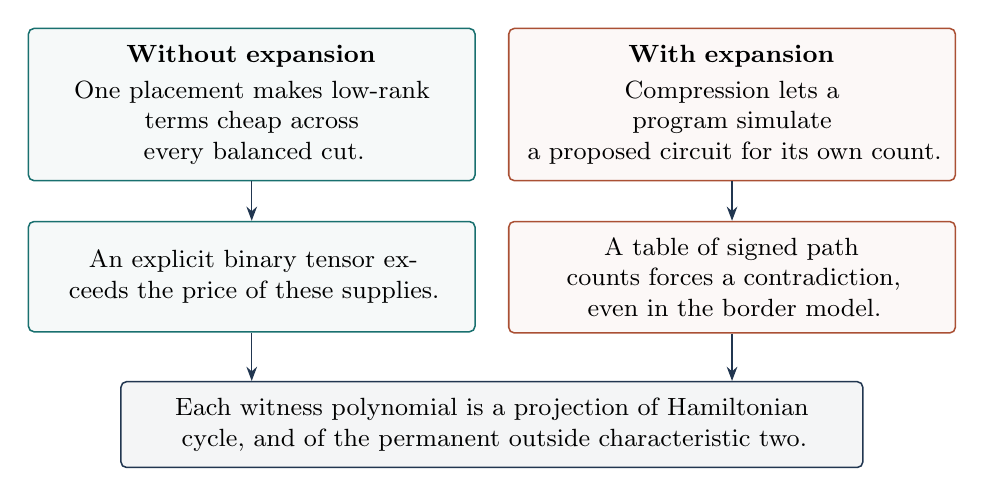
\begin{tikzpicture}[
  font=\small,align=center,
  branch/.style={draw=#1,fill=#1!4,rounded corners=2pt,line width=.55pt,
                 inner xsep=6pt,inner ysep=6pt,text width=5.25cm,minimum height=14mm},
  finish/.style={draw=ink,fill=ink!5,rounded corners=2pt,line width=.55pt,
                 inner sep=6pt,text width=9.0cm},
  arrow/.style={-{Stealth[length=1.8mm]},draw=ink,line width=.55pt}]
\node[branch=sea] (geom) at (-3.05,0)
  {\textbf{Without expansion}\\[2pt]
   One placement makes low-rank\\ terms cheap across every balanced cut.};
\node[branch=rust] (comp) at (3.05,0)
  {\textbf{With expansion}\\[2pt]
   Compression lets a program simulate\\ a proposed circuit for its own count.};
\node[branch=sea,below=5mm of geom] (binary)
  {An explicit binary tensor exceeds
   the price of these supplies.};
\node[branch=rust,below=5mm of comp] (signed)
  {A table of signed path counts forces a contradiction, even in the border model.};
\node[inner sep=0pt,outer sep=0pt,fit=(binary)(signed)] (witnesses) {};
\node[finish,below=6mm of witnesses] (both)
  {Each witness polynomial is a projection of Hamiltonian cycle,
   and of the permanent outside characteristic two.};
\draw[arrow] (geom)--(binary);
\draw[arrow] (comp)--(signed);
\draw[arrow] (binary.south)--(binary.south|-both.north);
\draw[arrow] (signed.south)--(signed.south|-both.north);
\end{tikzpicture}
\caption{The two witnesses for Theorem~\ref{thm:main}. Each verifier
gives a projection at polynomially larger order
(Lemma~\ref{gadget:verifier}). The counting argument also gives a
stretched-exponential bound in the characteristics where it applies
(Theorem~\ref{thm:stretch}).}
\label{fig:plan}
\end{figure}


\paragraph{When expansion fails.}
Consider a polynomial that uses one variable from each of $d$ rows in
every monomial. Its coefficients form a tensor with one index per row.
A small circuit expresses this tensor as a sum of terms, each of low
matrix rank across some balanced partition of the rows. The cut may
change from term to term. On four rows, take the product of wires on
$12$ and $34$, then add a second product on $13$ and $24$, using
disjoint local supports. Each term has rank one across its own cut.
Every balanced cut severs both wires of at least one term, so their
sum can have large rank across every cut.

Part~\ref{part:no} chooses \emph{one placement of the rows} at which
every low-rank term is cheap to supply. Start with all suppliers at the
center and the rows at unit distance. For each balanced cut, move two
suppliers towards their respective rows. A rank-$R$ term pays for one
wire of dimension $R$ between the suppliers, but saves on transport to
the rows. Every balanced cut saves order
$d/\sqrt{\log d}$ in transport per unit separation, to first order.
In Euclidean space some bisection of any centered set of unit vectors
gains only $O(\sqrt d)$, by averaging over random bisections. Failure of
expansion yields directions with the larger gain through an entropy
inequality for random walks. A product construction combines these
directions for all cuts (Sections~\ref{sec:poincare}--\ref{sec:lamps}).

At those same sites we need a tensor that costs nearly as much as
sending all its indices from the center. Exterior multiplication gives
tensors of minors whose prices can be estimated through dimensions of
intersections of subspaces. We construct one explicit tensor
with coefficients in $\{0,1\}$ from which a suitable tensor of minors
can be obtained at every such placement
(Sections~\ref{sec:exterior}--\ref{sec:packing}). Its price exceeds
the price of a sum of cheap supplies, even after accounting for the wire
that tells every row which summand to use. The comparison also works on
every grouped tensor power, keeping the degree at $d$ while the row
length grows. For fixed sufficiently large even $d$, this yields circuit size
$n^{\Omega(d/\sqrt{\log d})}$ in a variable budget $n$
(Corollary~\ref{cor:variable-budget}).
Letting $d$ grow gives the exponent of Theorem~\ref{thm:main}.

\paragraph{When expansion holds.}
In Part~\ref{part:port} the same geometry yields identities that
compress a tensor network while preserving its value \cite{oaG}.
Here a coefficient of the witness is the signed number of computation
paths of a program on a specified input. A sufficiently small network
for its coefficient table would let a program use compression to
simulate its own count within its allotted time and add one. The
contradiction depends on which work the program must do itself and which
it can delegate to the branches it counts. Sections~\ref{sec:compr}--%
\ref{sec:batches} establish this distinction and give a lower bound
even for networks computing batches of independent copies of the table
over a finite field (Theorem~\ref{thm:batches}). This use of an
algorithm to prove hardness has precedents in circuit complexity
\cite{ki,williams} and in tensor-network algorithms for satisfiability
\cite{falseeth,Anthropic}.

A border circuit poses a further problem. A coefficient that has a
finite boundary value can be a sum of terms with poles. On an algebraic
curve through the boundary point we use residues and the Cartier
operator to recover the coefficient as an eigenvalue of an explicitly
accessible matrix. The program can now perform its counting
contradiction one matrix entry at a time. For characteristic zero,
specialization to a suitable prime preserves the finite data needed by
the simulation (Sections~\ref{sec:parse}--\ref{sec:border}).
In every characteristic $\chi$ admitting ports, this argument gives
the stronger bound $2^{N^{\varepsilon_\chi}}$, for some
$\varepsilon_\chi>0$, on $\HC_N$ and, when $\chi\ne2$, on $\Per_N$
(Theorem~\ref{thm:stretch}).

\clearpage
{\small\tableofcontents}
\clearpage
\section{Tensor prices and wire distances}\label{sec:prices}

A tensor network supplies a coefficient array by sending labels along
wires and contracting tensors at their endpoints. A price assigns a
number to the array once its indices have been placed at sites. Local
linear maps can only decrease that number, and the prices of independent
wires add. Thus the wires in a network must together pay at least the
price of its output. We will also need the cost of two operations on a
network, moving an output index and summing several possible supplies.
Throughout this section and Part~\ref{part:no}, we use natural logarithms
for prices. This multiplies the base-two prices of \cite{oaG} by
$\log 2$ and preserves the units of wire distance.

\subsection{Local maps, placements and limits of tensors}

Fix a field $K$ and a finite set $J$ of at least two sites. A
\emph{restriction} acts on a tensor by a linear map at each site
(or by precomposition when the tensor is viewed as a multilinear
form). Two operations combine tensors on $J$. The tensor product
groups the corresponding factors at each site. The direct sum places
the two tensors in disjoint blocks of the local spaces. Up to mutual
restriction, these operations form the tensor semiring in Strassen's
asymptotic spectrum \cite{Strassen}.

A \emph{spectral point} $\varphi$ is a nonnegative real-valued
function on this semiring. It is monotone under restriction,
multiplies on tensor products, adds on direct sums, and preserves
zero and one. Matrix rank after flattening across a fixed nontrivial
bipartition is one example. Choose a scale $D>0$ and put
$H(T)=D\log\varphi(T)$, with $H(0)=-\infty$. Every nonzero tensor
restricts to a nonzero simple tensor, so $H(T)\ge0$ for $T\ne0$.

To share one label with $q$ possible values among the sites of a
nonempty $A\subseteq J$, use the diagonal tensor
\[
 \Delta_A(q)=\sum_{i=1}^q\bigotimes_{a\in A}e_i,\qquad
 \delta(A)=H(\Delta_A(2))/\log 2 ,
\]
with one-dimensional slots outside $A$. Tensor products multiply
label sizes, and restriction can reduce them. Comparing powers of
$q$ with powers of two therefore gives $H(\Delta_A(q))=\delta(A)\log q$.
In particular $\delta(J)=D$, since $\Delta_J(q)$ is the direct sum of
$q$ unit tensors. For $a\ne b$, the two-site diagonal is a wire from
$a$ to $b$. Its rate $d(a,b)=\delta(\{a,b\})$ defines a pseudometric
when $d(a,a)=0$. Joining two wires gives the triangle inequality.
A diagonal restricts to a wire between any pair of its sites.
Conversely, equating the labels on the edges of a tree spanning $A$
supplies the diagonal, even if the tree uses auxiliary vertices.
Consequently
\[
    \operatorname{diam}(A)\leq\delta(A)\leq
    \sum_{uv\ \mathrm{in\ the\ tree}}d(u,v).
\]

In a \emph{spectral space}, every finite set $A$ of positive diameter
carries a price $H_A=\delta(A)\log\varphi_A$ that induces the given
wire distances. The prices agree when one adds one-dimensional slots,
and a nonzero tensor supported at a single site has price zero. The
metric quotient of the sites of any spectral point carries this
structure \cite[Section~\ext{G}{sec:spectra}]{oaG}. A \emph{placement}
$x=(x_i)$ assigns each index of a tensor $T$ to a site. Group indices
assigned to the same site and write $H(T;x)$ for the resulting price.
A local map may act jointly on all indices at its site.

\par\Needspace{6\baselineskip}
\begin{lemma}[Price inequalities]\label{price:rules}
Let $T\ne0$ have local dimensions $q_i$ and let $x,y$ be two placements
in one spectral space. Then
\begin{equation}\label{price:transport}
   |H(T;x)-H(T;y)|\leq\sum_i d(x_i,y_i)\log q_i .
\end{equation}
For $L\ge1$ tensors of the same format at sites in $A$,
\begin{equation}\label{price:sum}
    H\left(\sum_{j=1}^L T_j\right)
       \leq\max_j H(T_j)+\delta(A)\log L.
\end{equation}
At fixed placement and format over an algebraically closed field, every
price sublevel is Zariski closed.
\end{lemma}

\begin{proof}
A wire of dimension $q_i$ can transport index $i$ from $x_i$ to $y_i$
by a contraction. Reversing the move proves Equation~\eqref{price:transport}.
Folding the local summand spaces takes a direct sum to an ordinary
sum. Apply additivity of $\varphi_A$ and take logarithms to obtain
Equation~\eqref{price:sum}. At a single site every nonzero sum has
price zero.

For closedness, let $U$ lie in the closure of a set of tensors of
price at most $b$ in an ambient tensor space of dimension $v$.
For every $h\ge1$, the map $T\mapsto T^{\otimes h}$ is polynomial.
The span of its values on the set is closed and hence contains
$U^{\otimes h}$. Expanding in degree-$h$ monomials in the entries
of $T$ bounds the dimension of this span by
$\binom{v+h-1}{v-1}$. Express $U^{\otimes h}$ in a basis of such
powers. Scaling a tensor by a nonzero constant preserves its price.
Equation~\eqref{price:sum} thus gives
\[
 hH(U)\le hb+\delta(A)\log\binom{v+h-1}{v-1},
\]
where $A$ is the set of occupied sites. Dividing by $h$ and letting
$h\to\infty$ proves the claim
\cite[Lemma~\ext{G}{lem:spectral-closure}]{oaG}
(see also \cite{SpectralSublevels}).
\end{proof}

For a network with fixed output sites, applying its local coefficient
tables to the product of its wire tensors supplies the output by
restriction. The sum of the wire prices therefore bounds the output
price, including in a limit at the same format. If a network shares
one label across several sites, its contribution is the corresponding
diagonal price. Equation~\eqref{price:sum} gives the same charge for
the common label selecting a summand.

\subsection{The spaces of wire distances}

A Hadamard space is a complete geodesic $\operatorname{CAT}(0)$ space.
Every spectral space extends isometrically to a Hadamard spectral
space that preserves its prices. The price of a nonzero tensor is
convex as its indices move simultaneously along constant-speed
geodesics. Three operations preserve spectral realizability. One can
rescale the metric and all prices by a common positive factor, pass
to a closed convex subspace, or take a pointed ultralimit
\cite[Theorem~\ext{G}{thm:geometry}, Proposition~\ext{G}{prop:joint-convexity}
and Section~\ext{G}{sec:limits}]{oaG}. For an ultralimit,
Equation~\eqref{price:transport} bounds the price on bounded
configurations and ensures independence of the representing sequences.

Let $\mathcal X_\chi$ denote the class of Hadamard spaces admitting
spectral prices over a field of characteristic $\chi$. The geometry
depends only on $\chi$. Indeed, scalar extension preserves the
possible simultaneous spectral values of tensors over the subfield
\cite[Lemma~\ext{G}{lem:comparison}]{oaG}, and every binary wire is
defined over the prime field. Finite wire-distance tables suffice to
recover a spectral structure on a Hadamard space. Fix a basepoint
and take a pointed ultralimit of realizations of its finite subsets
containing that point. An ultrafilter containing every tail gives an
isometric copy of the space, to which the limiting prices restrict.
We may therefore work over an uncountable algebraically closed field
of the chosen characteristic.

A class of metric spaces \emph{admits ports} if regular multigraphs
of a single positive degree and unbounded orders satisfy a uniform
Poincar\'e inequality for squared distances in all its spaces, as in
Section~\ref{sec:intro}. We allow symmetric nonnegative integral arc
counts of the given row sum, including diagonal entries. The condition
for $\mathcal X_\chi$ is precisely port admission by $\chi$
\cite[Definition~\ext{G}{def:ports}]{oaG}. Taking a metric quotient,
duplicating sites, or rescaling their distances preserves the inequality.

\subsection{The cost of sharing the summand index}

The balanced-cut decomposition in Part~\ref{part:no} will have at most
$2^d$ summands for $d$ row sites in a unit ball. By
Equation~\eqref{price:sum}, the charge for choosing the summand
depends on the diagonal rate of the row sites. The tree bound can grow
linearly in the number of sites. In the spaces we use, the following
estimate reduces this growth to the square root of its logarithm.

If $\chi$ has no ports, Theorem~\ref{prod:main} gives a subclass of
$\mathcal X_\chi$ that still has no ports and is closed under finite
$\ell_2$ products, positive rescaling, closed convex subspaces and
pointed ultralimits. This subclass contains a nontrivial segment,
since a class of one-point spaces admits every port family. Rescaling
segments and taking a pointed limit gives a line. Products of lines
and pointed limits then give a copy of the separable Hilbert space
$\ell_2$ (pass to the closed convex subspace generated by the
coordinate directions). Thus for $Y$ in the subclass we can place a
configuration in $Y\times\ell_2$ at Hilbert coordinate zero and choose
spectral prices on the product.

When $Y$ is a metric cone with tip $o$, these prices can be made
positively homogeneous under radial dilations. For $T\ne0$ replace
$H(T;x)$ by
\[
       \lim_{s\downarrow0} H(T;s x)/s .
\]
Joint convexity and the zero price at the tip give the limit. It is
also an ultralimit of the rescaled spectral prices, so it has the
same wire metric and satisfies the spectral axioms. This construction
applies to products of cones as well.

\begin{lemma}[Diagonal price in a ball]\label{price:diagonal}
Let $A$ consist of $n\ge2$ sites in a ball of radius $r$ in a geodesic
metric space $Y$. Equip $Y\times\ell_2$ with spectral prices, and
place the sites at Hilbert coordinate zero. Then
\[
  \delta(A)\leq \sqrt{2\pi}\,r n\,
  \phi\bigl(\Phi^{-1}(1-1/n)\bigr)=O(r\sqrt{\log n}),
\]
where $\Phi$ and $\phi$ are the standard normal distribution function
and density.
\end{lemma}

\begin{proof}
Rescale to $r=1$, since the claim at $r=0$ is immediate. Write $o$
for the ball center. We will compare the marginal cost of adding
each $a\in A$ to a ball in the Hilbert coordinates through $o$. Each
comparison takes place in a Euclidean patch, the product of a single
geodesic segment $[o,a]$ with a finite-dimensional Euclidean space.

First we show that on any finite-dimensional convex Euclidean patch
the diagonal rate of a finite nonempty set $V$ equals its mean width,
\[
 W(V)=\sqrt{2\pi}\,\EE\max_{v\in V}\langle G,v\rangle,\qquad
 G\ \text{a standard Gaussian vector}.
\]
The flat law of \cite[Theorem~\ext{G}{thm:flatlaw}]{oaG} gives this
identity on an entire Euclidean space. At a relative interior point
$y$ of a patch, each tangent rescaling limit contains its whole
translation space. Hence for every finite nonempty configuration $E$
of directions in that space,
\[
          \lim_{h\downarrow0}\delta(y+hE)/h=W(E).
\]
To pass from tangent configurations to $V$, work in its convex hull.
Adjoining any point of this hull preserves price. Indeed, the added
leg can be copied at any existing site, and its price is convex
in its position. Discarding the added leg gives the reverse inequality.
Choose a relative interior point as origin and
adjoin it to $V$. Thus $t\mapsto\delta(tV)$ has right derivative
$W(V)$ at $t=0$.

To bound its derivative at $0<t<1$, adjoin $(t+h)v$ to $tV$ for
each $v\in V$ in turn. Write $y=tv$ and $E=tV-y$, so $0\in E$.
For fixed $M>0$ and small $h>0$, the smaller configuration
$y+MhE$ lies in the convex hull of $tV$ and contains $y$. Adjoin
it at zero additional cost. Submodularity on intersecting sets
\cite[Proposition~\ext{G}{lem:submod}]{oaG} now bounds the increment
from adding $y+hv$ by the same increment starting from $y+MhE$
alone. The point $y$ is interior relative to the hull of $V$. After
division by $h$, the latter increment tends to
\[
             W(ME\cup\{v\})-W(ME).
\]
Let $M\to\infty$. Since $0\in E$, dominated convergence gives the bound
\[
 \sqrt{2\pi}\,\EE\!\left[
   \langle G,v\rangle_+\,
   \mathbf1_{\{\max_{e\in E}\langle G,e\rangle=0\}}\right].
\]
The event means precisely that $v$ maximizes $\langle G,\cdot\rangle$
on $V$. Almost surely the maximizing point is unique, and its value
is nonnegative since $0$ is in the hull. Summing these increments over
$v$ bounds the right derivative of $\delta(tV)$ by $W(V)$.
Convexity and continuity now give $\delta(V)=W(V)$.

For $t\ge0$, take a finite net $F$ in the Euclidean ball of radius
$t/\sqrt j$ in $j$ Hilbert directions through $(o,0)$. Monotonicity
and submodularity give
\[
 \delta(A)\leq\delta(F)+
        \sum_{a\in A}\bigl(\delta(F\cup\{a\})-\delta(F)\bigr).
\]
Use the patch formula for $F$ and $F\cup\{a\}$. Sending the mesh to
zero at fixed $j$ gives the Gaussian maximum $t\|G_j\|/\sqrt j$ on
the ball, where $G_j$ is a standard $j$-dimensional Gaussian. The same Gaussian linear functional has
value at $a$ equal to $d(o,a)G$ for an independent standard normal $G$.
The ball maximum tends in mean square to $t$ as $j\to\infty$, so
\[
 \delta(A)\leq\sqrt{2\pi}\left(t+
          \sum_{a\in A}\mathbb E(d(o,a)G-t)_+\right)
       \leq\sqrt{2\pi}\left(t+n\mathbb E(G-t)_+\right).
\]
Taking $t=\Phi^{-1}(1-1/n)$ and integrating the normal density gives
the stated expression. Taking $t=\sqrt{2\log n}$ gives the order bound.
\end{proof}

The leading constant is sharp even on a Hilbert space. For $n$
orthogonal unit vectors the flat law gives
$\delta(A)=\sqrt{2\pi}\,\EE\max_{i\le n}G_i$ for independent standard
normals $G_i$. The normal tail estimate gives
$\EE\max_iG_i\sim\sqrt{2\log n}$, so both sides of the bound have
leading term $2\sqrt{\pi\log n}$ at radius one.


\part{One placement for all balanced cuts}\label{part:no}
\section{From balanced cuts to circuit lower bounds}\label{sec:comparison}

Each monomial of a set-multilinear polynomial uses one variable from
each of $d$ disjoint rows. If every row has length $q$, its coefficients form a
tensor $T$ indexed by $[q]^d$, where $[q]=\{1,\ldots,q\}$. Write
\[
 f_T(X)=\sum_{j_1,\ldots,j_d\in[q]} T_{j_1\cdots j_d}
                    X_{1,j_1}\cdots X_{d,j_d}.
\]
Taking a tensor power gives more variables without increasing the
degree. In $T^{\otimes h}$ each row index is a word of length $h$, so
$f_{T^{\otimes h}}$ still has degree $d$ and now has $dq^h$ variables. Brand et al.\ study the
asymptotic circuit complexity of these grouped powers \cite{BrandMany}.

\begin{theorem}[Explicit tensors of low degree]\label{thm:lowdegree}
There are an absolute positive integer $a$ and absolute constants $c,C>0$
with the following property. For every sufficiently large even $d$, set
$m=\lceil\log_2 d\rceil$ and $w=\lceil a d m^{3/2}\rceil$. There is a
tensor $T_d$ with entries in $\{0,1\}$ on $d$ rows of common side $q_0$,
with $w\le\log q_0\le Cw$, such that over every field $F$ whose
characteristic has no ports,
\[
  \bsz_F^{[d]}(f_{T_d^{\otimes h}})
       \ge \exp(c h d w/\sqrt m) \qquad(h\ge1).
\]
An entry of $T_d$ is computable in time polynomial in $w$, uniformly in $d$.
\end{theorem}

\begin{corollary}[Bounds in the number of variables]\label{cor:variable-budget}
Over every field whose characteristic has no ports, there is a uniform
$\VNP$ family on at most $n$ variables of degree
$d=\Theta(\log n/(\log\log n)^{3/2})$ and degree-component border size
at least $\exp(\Omega((\log n)^2/(\log\log n)^2))$ for all sufficiently
large $n$. For each fixed sufficiently large even $d$ and all
$n\ge d q_0(d)$, grouped powers of the same $T_d$ give a uniform
$\VNP$ family of degree $d$, using at most $n$ variables and requiring
size $n^{\Omega(d/\sqrt{\log d})}$ in this model.
\end{corollary}

To prove Theorem~\ref{thm:lowdegree}, we extract a sum of low-rank
tensors from a small circuit. The cut on which a summand has low rank
can vary with the summand. We place the rows once and bound the cost
of every summand at those same sites. A second estimate gives an
explicit tensor whose price exceeds the total cost of this sum unless
the circuit is large. We use natural logarithms for prices.

\subsection{Balanced cuts in a circuit}

A bipartition of $[d]$ is \emph{balanced} if each side has at least
$d/3$ rows. The matrix of a tensor on such a cut has rows indexed by
the choices on one side and columns indexed by the choices on the
other. Its rank is the least number of products across the cut whose
sum is the tensor. Allowing the cut to vary over all nontrivial
bipartitions in such a sum gives Naslund's partition rank
\cite{Naslund}. A related lower bound for multiplicative complexity
uses products across three blocks of sizes $d-2,1,1$
\cite{BrandKaskiWang}. A product on one cut can have large matrix
rank on another, which limits the information from testing a single
flattening (see \cite{egow} for barriers to matrix-rank methods).
Here the balanced-gate argument of arithmetic depth reduction
\cite{VSBR} ensures that each product can use a balanced cut.

\begin{lemma}[Balanced cuts]\label{lem:balanced}
For $d\ge4$, the coefficients that use one variable in each of $d$
rows of the output of a size-$s$ circuit form a sum of at most $2^d$
tensors. Each summand has rank at most $2^{O(d)}(s+1)$ on its own
balanced cut, with at most one summand per cut. For degree-component
border size $s$, the coefficient tensor lies in the closure of the
set of these sums.
\end{lemma}

\begin{proof}
Set any variables outside the designated rows to zero. At each gate
keep the component of row multidegree $\mathbf1_I$ for
every $I\subseteq[d]$. Sums and differences act componentwise. At a
product, sum over decompositions of $I$ into two disjoint row sets.
Every discarded monomial has degree at least two in some row and
cannot contribute to a later $\mathbf1_I$ component. Computing these
components gives a circuit of size $2^{O(d)}(s+1)$ with a
row set at each gate, including the empty row set for scalar gates.

Expand the full-set output into parse trees. In each tree follow the
selected branch at a sum or difference and the child with more rows
at a product, breaking ties by a fixed rule. Stop at the first gate
with at most $2d/3$ rows. Its row set has at least $d/3$ elements,
since a product step decreases the row count by at most half and an
additive step preserves it.

Group the trees by their stopping gate. Any parse below that gate
fits each context in the group, since the path choice uses only the
row sets and branches above it. The other factors in the context use
the complementary rows. Summing the group thus gives one product
across its cut, with the signs of differences included in the
expansion. Collect products from gates with the same cut to obtain
the rank bound. Extracting these coefficients from the degree-$d$
component is a linear map, so the decomposition gives the asserted
containment after taking closures.
\end{proof}

\subsection{Two price estimates at one placement}

Work over an uncountable algebraically closed extension $K$ of
$\overline F$. A lower bound over $K$ descends to $F$. For each
circuit architecture the coefficient map is polynomial in the
constants, and the kernel of its pullback on coordinate rings
commutes with scalar extension. There are finitely many architectures
at a fixed format and size.

\paragraph{One placement for every cut.}
Theorems~\ref{prod:main} and~\ref{lamp:certificate} supply $d$ unit
sites $x_1,\ldots,x_d$ in a Hadamard metric cone, with uniform
Cartan barycenter at the tip $o$. The barycenter minimizes the mean
squared distance to the sites. The cone has dilations $z\mapsto tz$
for $t\ge0$. Write $\|z\|=d(o,z)$ and
\[
 \langle x,z\rangle=\tfrac12\bigl(\|x\|^2+\|z\|^2-d(x,z)^2\bigr).
\]
The cone distance law gives $\langle x,tz\rangle=t\langle x,z\rangle$
\cite{BH}. For a cut $\ell$, let $b_\ell(i)\in\{0,1\}$ indicate
the side containing row $i$. The same theorems give two points
$Z_{\ell,0},Z_{\ell,1}$ for each cut, at distance at most one, with
\begin{equation}\label{eq:score}
 \max_b\|Z_{\ell,b}\|=O(\sqrt d),\qquad
 \sum_i\langle x_i,Z_{\ell,b_\ell(i)}\rangle
                       \ge c_0 d/\sqrt m .
\end{equation}
The norm bound uses the fact that there are at most $2^d$ cuts.
The sum in Equation~\eqref{eq:score} measures the first-order decrease
in total distance to the rows when two suppliers move away from $o$
along their respective rays. We take the product with a Hilbert space
and choose homogeneous prices as in Section~\ref{sec:prices}.
Lemma~\ref{price:diagonal} bounds the price of sharing an $L$-valued
label among the row sites by $O(\sqrt m\log L)$.

\paragraph{A tensor that nearly attains the star bound.}
For any integer $dm\le w\le d^2$, Theorem~\ref{pack:witness} supplies
a single binary tensor $T$ of log side $\Theta(w)$. A local linear
map on each row takes $T$ to a tensor $\widehat U$ over $K$ whose
choice can depend on the priced placement. Each row of $\widehat U$
has the same finite alphabet $V$, with a real weight $t(v)$ attached
to each letter $v$. In a grouped power the weight of a word is the
sum of its letter weights. To price a tensor $A$ in these bases,
take the best sector of $A^{\otimes k}$ with prescribed word weight
in each row, adding the total prescribed weight to its ordinary
price. The limit of this maximum divided by $k$ is the weighted price
$\mathcal B_x(A)$ of Equation~\eqref{pack:weighted}.

Theorem~\ref{pack:witness} gives a function $\mathcal F$ on positive
distances with
\begin{align}
 \mathcal B_x(\widehat U)&\ge d\mathcal F(1)-O(d),&
 r\log\sum_{v\in V} e^{t(v)/r}&\le \mathcal F(r),\nonumber\\
 \mathcal F'(1)&=\Theta(w),&
 \sup_{1/2\le r\le2}|\mathcal F''(r)|&=O(w).
 \label{eq:pack-interface}
\end{align}
A supplier at the tip can send each index distance one to its row.
The resulting star has weighted price bounded by $d\mathcal F(1)$.
The witness comes within $O(1)$ per row of this benchmark.
Lemma~\ref{pack:value} gives the corresponding rules for comparing
supplies. Weighted prices add on grouped products and have closed
sublevels. Summing $L$ tensors costs at most their largest weighted
price plus the price of sharing an $L$-valued label. Sending an index
distance $r$ adds at most $r\log\sum_{v\in V}e^{t(v)/r}$ to the
ordinary price at the suppliers.

\begin{proof}[Proof of Theorem~\ref{thm:lowdegree}]
Let $s$ be the degree-component border size of $f_{T^{\otimes h}}$.
Lemma~\ref{lem:balanced} puts $T^{\otimes h}$ in the closure of
sums over balanced cuts with rank at most $2^{O(d)}(s+1)$ per cut.
Applying the local maps to obtain $\widehat U^{\otimes h}$ preserves
this conclusion. The maps are linear on coefficient arrays and can
only decrease cut ranks. The same conclusion holds if one starts
with a size-$s$ border circuit for $f_{\widehat U^{\otimes h}}$ over
$K$. We bound $s$ in either case.

For a term of rank $R\ge1$ on cut $\ell$, place two suppliers at
$y_b=\tau Z_{\ell,b}$ for a positive $\tau$ to be chosen. A rank
factorization represents the term by one wire carrying a label in
$[R]$, with one factor computed at each end. Since the suppliers
are at distance at most $\tau$, the wire costs at most $\tau\log R$.
Send each grouped index from its supplier to its row. Its sum of
exponential weights factors over the $h$ letters of a word.
Equation~\eqref{eq:pack-interface} therefore bounds the term's
weighted price by
\begin{equation}\label{eq:cut-price}
 \tau\log(s+1)+O(\tau d)+h\sum_{i=1}^d \mathcal F(r_i),\qquad
 r_i=d(x_i,y_{b_\ell(i)}).
\end{equation}
Figure~\ref{fig:supply} compares the two networks.
\begin{figure}[tbp]
\centering
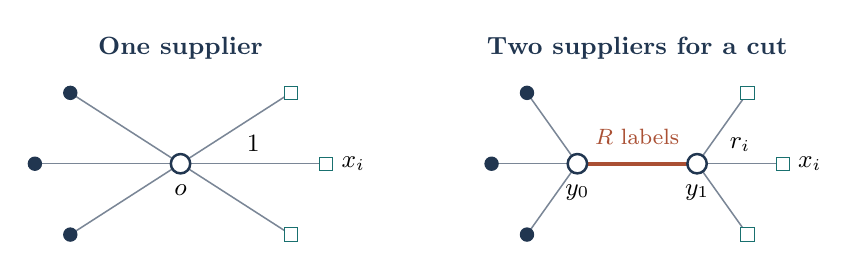
\begin{tikzpicture}[x=1cm,y=1cm,font=\small,
  row zero/.style={circle,draw=ink,fill=ink,inner sep=0pt,minimum size=4.8pt},
  row one/.style={rectangle,draw=sea,fill=white,inner sep=0pt,minimum size=4.8pt},
  supplier/.style={circle,draw=ink,fill=white,inner sep=0pt,minimum size=7pt,line width=.9pt},
  leg/.style={draw=ink!60,line width=.55pt},
  rank wire/.style={draw=rust,line width=1.5pt}]
\foreach \panel/\shift in {star/0,cut/5.8}{
  \begin{scope}[xshift=\shift cm]
    \foreach \i/\xx/\yy in {1/1.4/.90,2/1.85/0,3/1.4/-.90}{
      \coordinate (\panel-l\i) at (-\xx,\yy);
      \coordinate (\panel-r\i) at (\xx,\yy);
    }
  \end{scope}
}
\node[text=ink] at (0,1.47) {\textbf{One supplier}};
\node[text=ink] at (5.8,1.47) {\textbf{Two suppliers for a cut}};
\coordinate (origin) at (0,0);
\coordinate (supplier0) at (5.04,0);
\coordinate (supplier1) at (6.56,0);
\foreach \i in {1,2,3}{
  \draw[leg] (origin) -- (star-l\i);
  \draw[leg] (origin) -- (star-r\i);
  \draw[leg] (supplier0) -- (cut-l\i);
  \draw[leg] (supplier1) -- (cut-r\i);
}
\draw[rank wire] (supplier0) -- (supplier1)
   node[midway,above=3pt,font=\footnotesize,text=rust] {$R$ labels};
\path (origin) -- (star-r2) node[midway,above=1pt] {$1$};
\path (supplier1) -- (cut-r2) node[midway,above=1pt] {$r_i$};
\foreach \panel in {star,cut}{
  \foreach \i in {1,2,3}{
    \node[row zero] at (\panel-l\i) {};
    \node[row one] at (\panel-r\i) {};
  }
  \node[right=2pt] at (\panel-r2) {$x_i$};
}
\node[supplier,label=below:$o$] at (origin) {};
\node[supplier,label=below:$y_0$] at (supplier0) {};
\node[supplier,label=below:$y_1$] at (supplier1) {};
\end{tikzpicture}
\caption{Two supplies on the same row sites, drawn schematically for one
copy. Filled circles and open squares indicate the two sides of a balanced cut.
At the tip $o$, the total cost of the legs is at most $d\mathcal F(1)$.
Placing a supplier $y_b$ on each side reduces the sum of the leg bounds
to $\sum_i\mathcal F(r_i)$, where $r_i$ is the distance from $x_i$ to
its supplier. The rank index travels on the wire joining the suppliers
at a cost of at most $\tau\log R$.}
\label{fig:supply}
\end{figure}


Set $\tau=\eta/(d\sqrt m)$ for a sufficiently small absolute $\eta>0$.
The cone distance law at a unit site gives
$r_i=1-\tau\langle x_i,Z_{\ell,b_\ell(i)}\rangle+O(\tau^2d)$
and $|r_i-1|=O(\tau\sqrt d)$. Using the two derivative estimates of
Equation~\eqref{eq:pack-interface} and the sum in Equation~\eqref{eq:score}
gives
\[
 \sum_i \mathcal F(r_i)\le d\mathcal F(1)
                 -c_0\mathcal F'(1)d\tau/\sqrt m+O(w\tau^2d^2)
               \le d\mathcal F(1)-c_1 w/m .
\]
The linear term saves order $\eta w/m$. Its error is $O(\eta^2w/m)$,
so the same choice of $\eta$ gives the saving on every balanced cut.

There are at most $2^d$ terms. Summing them costs $O(d\sqrt m)$ once,
even for $h$ copies, and closedness preserves the resulting bound on
$\widehat U^{\otimes h}$. Its weighted price is at least
$h(d\mathcal F(1)-O(d))$ by additivity. Cancel the common contribution
$hd\mathcal F(1)$ to obtain
\begin{equation}\label{eq:balance-cost}
    \tau\log(s+1)+O(hd+d\sqrt m)\ \ge\ c_1 h w/m .
\end{equation}
Take $w=\lceil a d m^{3/2}\rceil$. For sufficiently large absolute
$a$ the saving $c_1 h w/m$ absorbs both errors for every $h\ge1$,
and $dm\le w\le d^2$ for all sufficiently large $d$. Dividing by
$\tau$ yields
\begin{equation}\label{eq:packed-hardness}
 \bsz_K^{[d]}(f_{\widehat U^{\otimes h}})
       \ge \exp(c_2 h d w/\sqrt m)
\end{equation}
and the same bound for $f_{T^{\otimes h}}$ over $F$.
The entry algorithm and the side bounds follow from
Theorem~\ref{pack:witness}.
\end{proof}

\subsection{From the explicit tensor to complete polynomials}

\begin{proof}[Proof of Corollary~\ref{cor:variable-budget}]
The construction in Theorem~\ref{pack:witness} pads the row alphabets
of $T_d$ with zeros to the predetermined size
$q_0(d)=2^{\lceil C'w\rceil}$ for a fixed absolute integer $C'$.
For a variable budget $n$, take the largest even $d$ with
$d q_0(d)\le n$. Maximality gives $n<(d+2)q_0(d+2)$, and increasing
$d$ to $d+2$ changes $w$ by at most a constant factor. Thus
$w=\Theta(\log n)$ and
$d=\Theta(\log n/(\log\log n)^{3/2})$. At $h=1$,
Theorem~\ref{thm:lowdegree} gives
\begin{equation}\label{eq:vnphard}
   \log \bsz_F^{[d]}(f_{T_d})
        =\Omega\!\left(\frac{(\log n)^2}{(\log\log n)^2}\right).
\end{equation}
For fixed sufficiently large even $d$ and $n\ge d q_0(d)$, use the
largest $h$ such that $d q_0(d)^h\le n$. Then
$h\log q_0(d)\ge\tfrac12\log(n/d)$ and $n\ge d^2$, giving
$n^{\Omega(d/\sqrt{\log d})}$.

For uniform $\VNP$ membership, guess the address of one variable in
each row, compute the tensor entry, and accept if it is one. In a
grouped power, the entry is the product of the individual bits. Each
accepting address contributes the product of its selected variables.
The Boolean computation has size polynomial in $n$. To express it
as a Valiant sum \cite{Valiant}, also guess its gate values and check
each bounded-fan-in gate by a constant-degree truth-table polynomial.
Each address has a unique consistent assignment of gate values.
The same construction supplies one output bit per address in each
row, indicating which variable to use. The resulting summand has
polynomial degree and circuit size. These Boolean tests work over
every characteristic.
\end{proof}

The completeness projections of Valiant \cite{Valiant,Burgisser}
transfer the lower bound to the two cycle polynomials. We give the
weighted verifier construction here because Part~\ref{part:port}
also needs control of degrees and of the arcs carrying variables.

\subsubsection{Preserving the variables in completeness projections}\label{sec:gadgets}

We use an explicit form of Valiant's completeness reductions
\cite{Valiant} to control the order of the graph and the placement of
the variables. A \emph{weighted Boolean verifier} is a circuit of fixed
bounded fan-in that takes Boolean guesses, tests acceptance, and computes
a list of output bits. Each listed bit has a weight in $F$ or a variable
weight. The verifier sums, over accepted guesses, the product of the
weights of the listed bits that are true. Each variable occurs once in
the list. Let $s$ count guesses, gates, wires and listed bits.

\begin{lemma}[Sparse completeness projections]\label{gadget:verifier}
The value of a weighted Boolean verifier of length $s$ is a projection
of $\HC_M$ with $M=O(s+1)$. Its directed graph has maximum indegree
and outdegree at most three. Each variable labels a single arc, and
these arcs have disjoint endpoints. If $\operatorname{char} F\ne2$,
the value is also a projection of $\Per_M$ for an order $M=O(s+1)$.
Its bipartite graph has maximum degree three and its variable edges
form a matching. Both constructions take polynomial time.
\end{lemma}

\begin{proof}
First encode the computation by clauses requiring exactly one true
literal. For each gate, introduce one indicator for each row of its
truth table and require exactly one indicator to hold. For each bit $x$
incident to the gate, form another clause from $\neg x$ and the
indicators of the rows in which $x=1$. The clause forces the selected
row to agree with $x$. Unit clauses fix constants and require
acceptance. Give every listed output a private copy $b$ of its bit $x$
using the clause $(\neg x,b)$. Every accepted guess then has exactly
one extension to a satisfying assignment, with its original weight.

There are $O(s+1)$ literal occurrences. To ensure that every clause
has length at most three, replace a long clause on
$\ell_1,\ldots,\ell_t$ by the clauses $(a_{j-1},\ell_j,\neg a_j)$
for $1\le j\le t$. Unit clauses fix $a_0=0$ and $a_t=1$. On Boolean
values these constraints say $a_j=a_{j-1}+\ell_j$ over the integers,
so the running sums give a unique extension precisely when one literal
is true. Finally add a private bit pinned true to cover the empty
verifier.

\smallskip\noindent\emph{Hamiltonian cycles.}
Make one bidirectional path per bit, and arrange the paths in cyclic
order. Put a connector between each path and the next, with incoming
arcs from either endpoint of the first path and outgoing arcs to either
endpoint of the next. Forward traversal represents true. On each path,
reserve one edge (a gap) per literal occurrence. The ordinary path
segments on either side of a gap have length at least two, as does a
path with no gaps. For a literal of clause $C$, write $u,v$ for the gap
endpoints in the direction that makes the literal true. Keep the arc
$v\to u$ and replace $u\to v$ by $u\to C\to v$, where all literals
in $C$ share the clause vertex $C$. Give a private ordinary forward arc
on each listed bit's path its output weight. Every other permitted arc
has weight one and all missing arcs have weight zero.

An interior vertex of an ordinary segment must use its two distinct
neighbors in a Hamiltonian cycle, since a return to one neighbor would
close a two-cycle. Thus each whole segment is traversed in one
direction. Across a gap, $v\to u$ is both the only possible incoming
arc at $u$ and the only possible outgoing arc at $v$. If either end
needs this arc, it fills both positions. Otherwise $u$ needs an
outgoing arc across the gap and $v$ needs an incoming arc there, forcing
$u\to C\to v$. In particular a cycle cannot enter a clause at one
gap and return at another. Each path therefore has a consistent
orientation, and each clause vertex is visited once precisely when
one of its literals is true. A satisfying assignment determines one
directed cycle through the paths in their cyclic order, counted once
in $\HC_M$, with the prescribed weight. Clause lengths give the degree
bound, and weighted arcs on distinct paths have disjoint endpoints.

\smallskip\noindent\emph{Perfect matchings.}
For each bit make a simple even bipartite cycle of length at least four.
Its two alternating perfect matchings represent true and false. Reserve
one distinct edge for each literal occurrence in the matching that makes
the literal true. For a listed bit, weight one further edge of the true
matching by its output weight. For each clause, create a row and a
column, with one prospective edge between them per literal. We must
couple each prospective edge to its occurrence edge so that they are
selected together.

Delete each such pair of edges and add three private rows and three
private columns with weight matrix
\[
  A=\begin{pmatrix}
     \tfrac12&\tfrac12&-\tfrac12\\
     -1&-1&1\\
     1&1&1
  \end{pmatrix}.
\]
For the first deleted edge, join its row to private column $1$ and
private row $1$ to its column. For the second edge, use private column
and row $2$ in the same way. All four connecting edges have weight one.
Fix the connecting edges used by a matching. They must occupy equally
many private rows and columns for an internal completion to exist. If
they occupy none, the total internal weight is $\operatorname{per}(A)=1$. With
one row and one column occupied, deleting them leaves a permanent of
zero for all four choices from indices $1,2$. With both rows and both
columns occupied, the remaining entry is $A_{33}=1$. Thus the only
states that contribute are those using neither deleted edge or both,
each with factor one. This cancellation uses the inverse of $2$.

After summing over the private vertices, each clause chooses one literal
and each bit chooses an alternating matching. Their choices agree
exactly for satisfying assignments. The unweighted cycle edges carry
weight one and all missing edges carry weight zero. With these entries
the permanent equals the verifier sum.

The only vertices that can have degree four are private rows and columns.
Split any such row into two rows, give each two of its old edges, and
add one column adjacent to both with unit weights. Exactly one row
matches externally, and its choice forces the match to the new column.
Use the transposed operation for columns of degree four. This preserves
the permanent and leaves the variable edges on distinct bit cycles.
Both constructions use only a constant number of vertices per bit and
per literal occurrence, hence have order $O(s+1)$.
\end{proof}


\begin{proof}[Proof of Theorem~\ref{thm:main} in the absence of ports]
Apply Lemma~\ref{gadget:verifier} to the Boolean verifier for $f_{T_d}$
above. Its size is polynomial in $n$ with absolute constants. Thus
$f_{T_d}$ is a projection of $\HC_M$ with $M\le A n^b$ for absolute
$A,b$, and also of $\Per_M$ under the same bound outside
characteristic two. To obtain any larger order, split a vertex of
the Hamiltonian-cycle instance into a forced path, or add an identity
block to the permanent instance.

A projection that substitutes constants can mix homogeneous degrees.
Suppose the complete polynomial of order $N$ lies in the closure
of degree-$N$ components of size-$s$ circuit outputs. For each such
circuit compute all homogeneous components through degree $N$ at each
gate, using addition or convolution. The isolated
degree-$N$ output is a full homogeneous approximant of size
$O((N+1)^2(s+1))$. Project that output, then select its degree-$d$
component. Both maps on coefficients are linear, so a degree-component
border circuit for the complete polynomial gives the same border
upper bound $O((N+1)^2(s+1))$ for $f_{T_d}$.

For each sufficiently large $N$, choose $n=\lfloor(N/A)^{1/b}\rfloor$
and pad the projected instance to order $N$. Equation~\eqref{eq:vnphard}
now bounds $O((N+1)^2(s+1))$ from below. Since $\log n\sim b^{-1}\log N$,
its logarithmic lower bound dominates the $O(\log N)$ cost of
isolating the degree. This gives the claimed exponent with an
absolute constant.
\end{proof}

\begin{corollary}[Sparse supports]\label{cor:sparse-support}
The lower bound of Theorem~\ref{thm:main} holds on directed graphs of
order $N$ with indegree and outdegree at most three, and, for the
permanent outside characteristic two, on bipartite graphs of degree
at most three with $N$ vertices on each side. More precisely, in each
case there exists such a graph at every sufficiently large $N$, and
each allowed arc or edge carries its own independent variable. In a
characteristic admitting ports these graphs also attain the
stretched-exponential bound of Theorem~\ref{thm:stretch}.
\end{corollary}

\begin{proof}
In either branch apply Lemma~\ref{gadget:verifier} to the verifier
used in the transfer, here for $f_{T_d}$ and in Section~\ref{sec:border}
for the signed verifier. Keep independent variables on all permitted
arcs or edges and set the other entries of the complete matrix to zero.
The resulting degree-$N$ graph polynomial still projects to the verifier
polynomial by specializing the permitted entries. Padding a directed
vertex into a forced path puts its incoming arcs at the first vertex
and its outgoing arcs at the last, preserving both degree bounds.
Padding a bipartite graph by disjoint edges preserves its maximum
degree as well. The same homogeneous extraction before specialization
therefore transfers the verifier lower bound to these graph polynomials
at every sufficiently large order.
\end{proof}

\section{A logarithmic lower bound for the Poincaré constant}\label{sec:poincare}

The price comparison in Section~\ref{sec:comparison} requires a
single placement of the row sites that works for every balanced cut.
To construct it, we shall look for placements that make two random
changes of state have very different mean squared lengths. The
simplest comparison is on a regular graph. One step follows an edge,
and the other goes to an independent uniform vertex. If a class of
Hadamard spaces has no ports, the constant that bounds the second
energy by the first is at least of order \(\log n\) on \emph{every}
\(n\)-vertex graph of bounded degree. This bound will allow us to
distinguish two walks by the information they generate.

For a finite Markov kernel \(P\) with stationary law \(\pi\) and a
placement \(x=(x_i)\) of its states, put
\[
 \mathcal E_P(x)=\sum_{i,j}\pi_iP_{ij}d(x_i,x_j)^2,\qquad
 \mathcal V_\pi(x)=\sum_{i,j}\pi_i\pi_j d(x_i,x_j)^2 .
\]
For a pair law \(D\), the weights in \(\mathcal E_D(x)\) are its joint
probabilities. Write \(\mathcal V\) when \(\pi\) is uniform. States
of zero stationary mass may be discarded. A \(d\)-regular multigraph
has a symmetric matrix of nonnegative integral arc counts with every
row sum \(d\). A holding arc counts once. Dividing the counts by
\(d\) gives the walk kernel with uniform stationary law.

Suppose one large graph had too small a Poincar\'e constant. Placing
a copy of it at each vertex of a preceding graph would multiply the
order at every iteration. To keep the Poincar\'e constants bounded,
we average the walk on the preceding graph before inserting the
copies. The estimate for this averaging is a form of nonlinear
spectral calculus \cite{MendelNaor,MendelNaorBarycentric}. We give
the barycentric argument for Hadamard spaces
\cite{BH,Sturm}.

\begin{lemma}[Smoothing a walk]\label{lem:power}
Let \(P\) be a finite Markov kernel with stationary law \(\pi\), and let
\(t\ge2\) be even. Put
\[
 A=\tfrac12(I+P),\qquad S=\tfrac1t\sum_{h=1}^t A^h .
\]
For each placement \(x\) in a Hadamard space \(X\) there is a placement
\(y\) in \(X\) such that
\begin{equation}\label{eq:hadamard-smoothing}
 \sum_i\pi_i d(x_i,y_i)^2+t\mathcal E_P(y)
 \le 16\mathcal E_S(x).
\end{equation}
If \(D\) has both marginals \(\pi\) and
\(\mathcal E_D\le\beta\mathcal E_P\) for all placements in \(X\), then
\(\mathcal E_D\le C(1+\beta/t)\mathcal E_S\) for all placements in \(X\),
with an absolute constant \(C\).
\end{lemma}

\begin{theorem}[Logarithmic Poincaré obstruction]\label{thm:loggraph}
Let \(P\) be the walk on a \(d\)-regular multigraph with \(n\ge2\)
vertices, \(d\ge1\), and uniform stationary law \(\pi\). Suppose
that \(\mathcal V_\pi(x)\le\beta\mathcal E_P(x)\) for every
placement \(x\) in every member of a class of Hadamard spaces
without ports. Then
\[
                 \beta\ \ge\ c\,\frac{\log n}{\log(d+1)}
\]
for an absolute constant \(c>0\).
\end{theorem}

\begin{proof}[Proof of Lemma~\ref{lem:power}]
The barycenter \(b\) of a finite probability measure \(\mu\) in \(X\)
satisfies the variance inequality
\(\int d(z,w)^2\,d\mu(w)\ge d(z,b)^2+\int d(b,w)^2\,d\mu(w)\).
Indeed the midpoint inequality makes any minimizing sequence Cauchy,
and squared-distance convexity along the segment from the minimizer
to \(z\) gives the displayed inequality.
Starting with \(x^0=x\), take \(x_i^{g+1}\) to be the barycenter of the
\(x_j^g\) with weights \(A_{ij}\). Put
\[
 q_g=\sum_{i,j}\pi_iA_{ij}d(x_i^{g+1},x_j^g)^2,\qquad
 u_g=\sum_i\pi_i d(x_i,x_i^g)^2 .
\]
Run the stationary \(A\)-walk for \(h\) steps. Conditional on the first
\(h-1\) steps, apply the variance inequality to the last point with
the starting point as \(z\). Replace the last point by its conditional
barycenter and repeat. At the \(g\)-th replacement, starting at
\(g=0\), stationarity makes the mean variance term equal to \(q_g\).
Consequently
\[
 \mathcal E_{A^h}(x)\ge u_h+\sum_{g=0}^{h-1}q_g .
\]
On averaging over \(1\le h\le t\), each \(q_g\) with \(g<t/2\)
occurs in at least \(t/2\) summands. Since \(u_0=0\),
\[
 \sum_{0\le g<t/2}\bigl(u_g+(t/2)q_g\bigr)\le t\mathcal E_S(x).
\]
Choose a summand of size at most \(2\mathcal E_S(x)\).
Comparison along \(x_i^g,x_i^{g+1},x_j^g\) gives
\(\mathcal E_P(x^g)\le4q_g\), because \(A\) averages a holding step
and a \(P\)-step. Taking \(y=x^g\) proves \eqref{eq:hadamard-smoothing}.
Finally
\(\mathcal E_D(x)\le3(2u_g+\mathcal E_D(y))\) by the two marginal
identities. Apply the assumed comparison at \(y\).
\end{proof}

\begin{proof}[Proof of Theorem~\ref{thm:loggraph}]
A class without ports contains a space with two distinct
points. Choose one of the points independently and uniformly at
each vertex, and average the asserted inequality. The expected pair
energy is \((1-1/n)\) times half their squared distance, and the edge
energy is at most half their squared distance. Thus \(\beta\ge1/2\).
Write \(b=\max(1,\beta)\) and call the given multigraph \(H\).

Fix an even \(t\ge2\) with \((2d+1)^t\le n/2\). Given a previous
graph of degree \(2d\) with walk \(K\) and Poincaré constant at most
\(\gamma\), form the averaged kernel \(S\) of Lemma~\ref{lem:power}
from \(K\). The new pair comparison for \(S\) has constant at most
\(C(1+\gamma/t)\) throughout the class.
We need a symmetric approximation to \(S\) whose probabilities have
denominator \(n\). In each row set \(m_{uv}=\lceil n S_{uv}/2\rceil\).
A row of \(S\) has support at most \((2d+1)^t\), since holds pad shorter
walks to length \(t\). Hence its integer row sum is at most
\(n/2+(2d+1)^t\le n\). Pad each diagonal entry to reach \(n\).
The counts remain symmetric and \(R_{uv}=m_{uv}/n\ge S_{uv}/2\).
It follows that the Poincaré constant of \(R\) is at most
\(\rho=2C(1+\gamma/t)\).

Replace each old vertex \(u\) by a copy of \(H\). Partition its \(n\)
vertices into sets of sizes \(m_{uv}\), and match the set indexed by
\(v\ne u\) bijectively to the set indexed by \(u\) in the copy at \(v\).
Fix the vertices in the set indexed by \(u\) itself. This gives an
involution whose projected step from a uniform vertex of the copy
has distribution \(R_{u\bullet}\).
The new graph has the \(d\) internal arcs of \(H\) at each vertex and
\(d\) copies of its involution arc. Its mean edge energy is
\((E_{\rm in}+E_{\rm match})/2\), with the two terms the corresponding
mean energies.

For a placement \(x\) in any one of the test spaces, let \(z_u\)
be the barycenter of the points in the copy at \(u\). Let \(v_0\) be
the mean squared distance to one's own barycenter. Minimization against
a uniformly chosen point in each copy and the comparison on \(H\)
give \(v_0\le b E_{\rm in}\). Apply the triangle inequality first from
one barycenter to the next via a matched pair, then between independent
vertices via their two barycenters. Uniformity of both endpoints of an
involution step gives
\[
 \mathcal E_R(z)\le3(2v_0+E_{\rm match}),\qquad
 \mathcal V(x)\le3(2v_0+\mathcal V(z)).
\]
Here each pair energy uses the uniform law on the indicated graph.
Since \(\mathcal V(z)\le\rho\mathcal E_R(z)\), the new graph has a
Poincaré bound \(B b(1+\gamma/t)\) for an absolute \(B\ge1\).

If \(Bb/t\le1/2\), iteration starting from one vertex with \(2d\)
loops gives graphs on \(n^k\) vertices of fixed degree \(2d\) with
bounds at most \(2Bb\). These graphs would be ports for the class.
Hence every admissible even \(t\) satisfies \(t<2Bb\). If
\(\log(n/2)/\log(2d+1)\ge4\), the largest admissible even \(t\)
is at least half this ratio. In the remaining range
\(\log n/\log(d+1)\) is bounded absolutely and \(\beta\ge1/2\)
suffices. Since \(b\le2\beta\), this proves the assertion.
\end{proof}

We shall apply the bound to walks with unequal transition
probabilities. Only the number of possible destinations matters.

\begin{corollary}[Symmetric kernels with sparse rows]\label{cor:support}
Suppose \(P\) is a symmetric stochastic matrix on \(n\ge2\) states
with at most \(d\) positive entries per row, where \(d\ge1\) is
an integer, and let \(\pi\) be uniform. If
\(\mathcal V_\pi(x)\le\beta\mathcal E_P(x)\) for every placement \(x\)
in every member of a class of Hadamard spaces without ports, then
\(\log n\le C\beta\log(d+1)\) for an absolute constant \(C\).
\end{corollary}
\begin{proof}
Take \(\lceil dP_{ij}\rceil\) arcs in each position and add holding
arcs to make every row sum \(2d\). The walk on the resulting symmetric
regular multigraph dominates \(P/2\) entrywise, so its Poincaré
constant is at most \(2\beta\). Apply Theorem~\ref{thm:loggraph}.
\end{proof}
\section{Observable entropy}\label{sec:entropy}

A graph of small degree gives a walker few choices at each step.
A walk with many possible destinations can also transmit little
information if a few choices carry most of the probability, or if
many destinations share the same observable label. We compare
two walks on the same state space. One, the \emph{demand} walk,
specifies the pairs of states we want far apart in a placement.
The other, the \emph{physical} walk, specifies the moves we want
short. A uniform comparison of their squared lengths bounds the
amount of information one demand step can generate about the
destination label, given the full starting state. The bound measures
the physical walk by the number of bits per observed label along a
long stationary trajectory.

Given a labeling $L$ of a finite set $V$ and a stationary $P$-walk
$(X_t)_{t\ge0}$ on $V$, put
\[
 H_j=H\big(L(X_0),\ldots,L(X_{j-1})\big),\qquad
 a=\lim_{j\to\infty}\frac{H_j}{j}=\inf_{j\ge1}\frac{H_j}{j}.
\]
Here \(H\) denotes Shannon entropy in bits, and all logarithms in this
section are in base two \cite{ct}. The equality follows from
stationarity and subadditivity of block entropy.

\begin{theorem}[Observable entropy]\label{thm:entropy}
Let $P,D$ be Markov kernels on a finite set with common stationary
law $\pi$. Suppose that $\beta\ge1$ and that
$\mathcal E_D(f)\le\beta\mathcal E_P(f)$ for every placement $f$ in
a class of Hadamard spaces without ports. For any labeling $L$, let $a$ be its entropy rate
for the stationary $P$-walk and draw $(X,Y)$ from the stationary
$D$-step. Then
\[
 H(L(Y)\mid X)\le C\beta(1+a)
\]
for an absolute constant $C$.
\end{theorem}

In particular, if the demand information exceeds \(C\beta(1+a)\)
for some \(\beta\ge1\), one of the target spaces admits a placement with
\(\mathcal E_D(f)>\beta\mathcal E_P(f)\). Section~\ref{sec:product}
uses the identity labeling on a walk of words modulo cyclic rotation.
The full state is then observable and the entropy rate is its
one-step conditional entropy. In Section~\ref{sec:lamps} the label
records only an array of lamps. The physical walk also keeps auxiliary
records, so the cost in Theorem~\ref{thm:entropy} is the entropy rate
of the observed arrays over time.

The additive constant accounts even for deterministic motion. If \(P\)
alternates between two states and \(D\) draws a uniform state
independently, the identity labeling gives \(H_j=1\) for every \(j\).
Here \(a=0\), yet \(H(Y\mid X)=1\) and
\(\mathcal E_D=\mathcal E_P/2\).

\begin{proof}
We may assume that the stationary $D$-step is exchangeable. Indeed,
replace its pair law by the average of that law and its transpose.
The squared energies are unchanged, and concavity of conditional
entropy in the joint law shows that the new $H(L(Y)\mid X)$ is at
least half the original value. The stationary $P$-walk is unchanged.

Write $h=H(L(Y)\mid X)$ for this symmetrized step and assume $h>0$.
We use \(r\) copies of the original state, called the reservoir, to
write entries in an array of \(m\) lamps. At each writing step the
value added to one lamp is a function of the reservoir labels.
From a set of starts of mass at least one half, a demand move in all
\(r\) cells yields an increment whose law dominates a fixed fraction
of the uniform law on \(\lfloor rh/4\rfloor\)-bit words. We shall use the assumed
comparison to charge a refresh of all the lamps to \(O(mr\beta)\)
physical steps. Corollary~\ref{cor:support} will then require the net
change over those steps to carry order \(mrh\) bits. A description
of the same change using only the observed reservoir labels and the
writing schedule gives the upper bound in terms of \(a\).

\smallskip\noindent
\emph{Extracting lamp values.}
Fix \(m\ge1\). Take \(r\) sufficiently large that \(r\ge2\) and
\(k=\lfloor rh/4\rfloor\ge1\).
Set $A=\mathbb F_2^k$ and $q=|A|$. Write $L^r$ for the coordinatewise
labeling. There is a function $b$ from $r$-tuples of labels to $A$
and a set $B\subseteq V^r$ of $\pi^r$-mass at least $1/2$ such that
for $U'\sim D^{\otimes r}(u,\cdot)$ one has
\begin{equation}\label{eq:lamp-hash}
 \Pr\{b(L^r(U'))=z\mid U=u\}\ge \frac1{4q}
 \qquad(u\in B,\ z\in A).
\end{equation}
To see this, draw $r$ independent stationary $D$-steps. The negative
logarithm of the conditional probability of their destination label
tuple, given the starting reservoir $U$, is the sum of $r$ independent
random variables of mean $h$. The law of large numbers implies that,
for a set of starts of mass $1-o(1)$, atoms of conditional probability
at most $2^{-3rh/4}$ carry at least half the conditional mass. Assign
each label tuple a uniformly random color in $A$, independently. At
any such start, the mass of these small atoms assigned to a given
color has mean at least $1/(2q)$ and variance at most $2^{-3rh/4}/q$.
Chebyshev's inequality and a union bound give failure probability at
most $16q^2 2^{-3rh/4}=o(1)$ for the lower bound $1/(4q)$ in all
colors. Averaging over the coloring gives~\eqref{eq:lamp-hash}.

\smallskip\noindent
\emph{Comparing two walks on lamps and reservoirs.}
The physical kernel $G$ has stationary law $\pi^r$ times the uniform
law on $A^m$. With probability $1-1/r$ it advances a uniformly chosen
reservoir cell by $P$. With the remaining probability it chooses a
uniform lamp $J$ and adds $b(L^r(U))$ to that lamp. The first operation
preserves $\pi^r$ by stationarity of \(P\), and the second permutes the
uniform array for every fixed reservoir.
The demand kernel $D_*$ keeps the reservoir fixed. It replaces all
lamps by independent uniform values if $U\in B$ and holds otherwise.
For every placement \(F\) of this enlarged state space in a member of
the class, we claim that
\begin{equation}\label{eq:lamp-compare}
 \mathcal E_{D_*}(F)\le Cmr\beta\,\mathcal E_G(F).
\end{equation}

We first compare a refresh of just one lamp with the three moves in
Figure~\ref{fig:lamp}. Write \(s\in A^m\) for the lamp array and
\(e_Jz\) for the array equal to \(z\) in position \(J\) and zero
elsewhere. At a good starting reservoir \(u\in B\), draw
\(u'\sim D^{\otimes r}(u,\cdot)\). Add \(z=b(L^r(u'))\) to lamp \(J\) and return the reservoir to \(u\).
The endpoint is \((u,s+e_Jz)\). By \eqref{eq:lamp-hash}, every
increment has probability at least \(1/(4q)\). Thus the endpoint
law dominates one quarter of the uniform replacement law.

\begin{figure}[tbp]
\centering
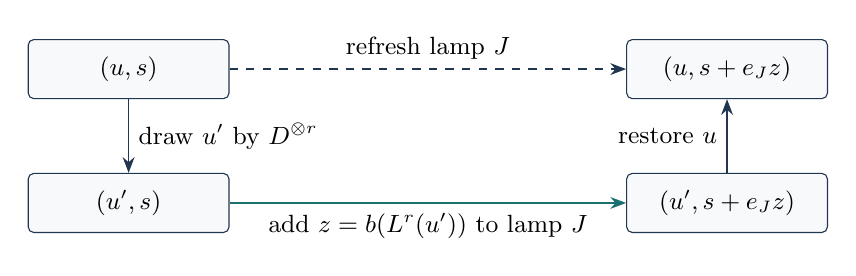
\begin{tikzpicture}[x=1cm,y=1cm,font=\small,
    state/.style={rectangle,rounded corners=2pt,draw=ink,
                  fill=ink!3,inner xsep=5pt,minimum width=2.55cm,
                  minimum height=7.5mm},
    move/.style={-{Stealth[length=2mm]},semithick,draw=ink}]
  \node[state] (ul) at (0,1.7) {\((u,s)\)};
  \node[state] (ur) at (7.6,1.7) {\((u,s+e_Jz)\)};
  \node[state] (ll) at (0,0) {\((u',s)\)};
  \node[state] (lr) at (7.6,0) {\((u',s+e_Jz)\)};
  \draw[move,dashed] (ul.east) -- node[above] {refresh lamp \(J\)} (ur.west);
  \draw[move] (ul.south) -- node[right] {draw \(u'\) by \(D^{\otimes r}\)} (ll.north);
  \draw[move,draw=sea] (ll.east) -- node[below] {add \(z=b(L^r(u'))\) to lamp \(J\)} (lr.west);
  \draw[move] (lr.north) -- node[left] {restore \(u\)} (ur.south);
\end{tikzpicture}
\caption{Refreshing lamp \(J\) while restoring the reservoir to its
initial state \(u\). The dashed step adds a uniform increment. On the
solid path the vertical moves are charged to the demand walk on the
reservoir cells, and the horizontal move is a single physical lamp
addition. For \(u\in B\), each endpoint of the dashed step occurs
along the solid path with at least one quarter of its probability.}
\label{fig:lamp}
\end{figure}

To pay for the outward reservoir move, we need the squared cost of
changing independent cells to be bounded by the sum of their
individual costs. If $(S_i,S'_i)$ are independent exchangeable
pairs and $S^{(i)}$ denotes $S$ with $S_i$ replaced by $S'_i$, then
\begin{equation}\label{eq:product-exchange}
 \mathbb E\,d(F(S),F(S'))^2
 \le\sum_i\mathbb E\,d(F(S),F(S^{(i)}))^2.
\end{equation}
For two blocks of coordinates form the quadrilateral obtained by
choosing the original or changed value in each block. The CAT$(0)$
quadrilateral inequality bounds the sum of squared diagonals by the
sum of squared sides. Exchanging one block preserves the joint law,
so the diagonals have equal expected squares, and each opposite pair
of sides does too. Dividing by two and iterating over the blocks
proves~\eqref{eq:product-exchange}.

Make independent $D$-moves in all $r$ reservoir cells, keeping the
lamps fixed. Under stationarity the squared cost of this change is at
most $2r\beta\,\mathcal E_G(F)$ by~\eqref{eq:product-exchange} and
the assumed comparison on each cell, since $1-1/r\ge1/2$. The squared
cost of a single random lamp addition is at most $r\mathcal E_G(F)$.
It remains to charge the return move. Integrate the path bound over
\(u\in B\), a uniform lamp array \(s\), and a uniform address \(J\).
The squared endpoint distance is at most three times the sum of the
squared lengths of the three legs. We bound this sum by integrating
over all starts. The first and last legs then have equal average cost,
since $s+e_Jz$ is uniform even conditional on $u,u',J$. The middle leg
has the stationary lamp-addition cost because \(u'\) has law \(\pi^r\).
Thus replacing one random lamp at good starts, with holding elsewhere,
costs at most $Cr\beta\,\mathcal E_G(F)$. Applying
\eqref{eq:product-exchange} to the $m$ independent pairs of old and
new lamp values at each good start gives~\eqref{eq:lamp-compare}.

\smallskip\noindent
\emph{Entropy forced by spreading the lamps.}
Take $T=2\lceil mr\beta\rceil$ and apply Lemma~\ref{lem:power}
to~\eqref{eq:lamp-compare}, using the Ces\`aro average of the lazy
$G$-walk up to time $T$. For placements depending only on the lamps,
the demand energy is $\pi^r(B)\mathcal V(f)$, where $\mathcal V(f)$
is the mean squared distance between images of two independent
uniform elements of $A^m$. The physical displacement of the lamps is
a random translation by some $Z\in A^m$, independent of their uniform
starting value $s$. All reservoir moves and choices of lamps are
independent of $s$. We obtain, with an absolute $K\ge1$,
\begin{equation}\label{eq:lamp-translation}
 \mathcal V(f)\le K\,\mathbb E\, d(f(s),f(s+Z))^2
 \qquad\text{for all placements } f \text{ in the class} .
\end{equation}

Each fixed translation has squared energy at most $4\mathcal V(f)$,
by the triangle inequality through an independent uniform point.
Put $\eta=1/(8K)$. Replace by zero every value of $Z$ whose probability
is less than $2^{-H(Z)/\eta}$. The replaced mass is at most $\eta$
by Markov's inequality for the information of the sampled atom (if
$H(Z)=0$ the support is a singleton). The discarded translations
contributed at most
\(4\eta\mathcal V(f)\) to the expectation in
\eqref{eq:lamp-translation}. Since \(4K\eta=1/2\), the resulting
translation kernel satisfies the same comparison with constant \(2K\).
It is symmetric because $A^m$ has exponent two, and each of its rows
has at most $1+2^{H(Z)/\eta}$ atoms. Corollary~\ref{cor:support}
therefore gives
\begin{equation}\label{eq:lamp-bits}
 mk=\log |A^m|\le C(1+H(Z)).
\end{equation}

\smallskip\noindent
\emph{Coding the physical displacement.}
In a trajectory of the lazy Ces\`aro walk, ignore lazy holds. There
are at most $T$ steps left. Let $S$ be the number of lamp additions,
so $\mathbb E S\le T/r$. Record $S$ in unary and the $S$ lamp
addresses in $\lceil\log m\rceil$ bits each. Within each of the $S+1$
intervals before, between and after additions, record in unary the
number of $P$-steps taken by each reservoir cell. The lengths of
these $r(S+1)$ unary words sum to at most $T+r(S+1)$ bits.
This prefix code for the schedule data has expected length at most
\[
 C\big(T+r+(T/r)\log(2m)\big).
\]
The order of moves in different cells inside an interval is
immaterial, since no lamp is read or written there.

Given the recorded data, the successive labels in a cell have the law
of a stationary $P$-block of the indicated length $j$, including its
initial label. This follows by constructing independent stationary
$P$-trajectories for the cells before sampling the schedule. Since
$H_j/j\to a$, there is $M_0<\infty$, depending only on $P,\pi,L$,
such that $H_j\le (1+a)j+M_0$ for every $j$. The $r$ lengths sum to
at most $T+r$. The schedule and these label blocks determine the
reservoir labels at every lamp addition and hence determine $Z$.
The chain rule for entropy now gives
\begin{equation}\label{eq:lamp-code}
 H(Z)\le C\big((T+r)(1+a)+rM_0+(T/r)\log(2m)\big).
\end{equation}
Combine~\eqref{eq:lamp-bits} and~\eqref{eq:lamp-code} and divide by
$mr$. Let $r\to\infty$ with $m$ fixed. The lamp-address contribution
tends to zero, and $k/r\to h/4$. Next let $m\to\infty$ to remove
$M_0/m$. As $T/(mr)\to 2\beta$ in the first limit, this proves the
theorem.
\end{proof}

\subsection{Conditional entropy of weighted edge laws}\label{sec:cursor-entropy}

For a graph with weighted edges, the demanded pairs and the
physical edges can have different vertex marginals. Symmetrize each
pair law and add suitable holding steps. The resulting walks have a
common stationary law and both squared energies are halved. Applying Theorem~\ref{thm:entropy} with the
identity labeling then bounds the one-step demand entropy.

\begin{corollary}[Pair laws on a graph]\label{cor:graph-entropy}
Let $\mu$ and $\alpha$ be laws on ordered pairs from a finite set, and
suppose that $\mathcal E_\mu(f)\le\beta\mathcal E_\alpha(f)$
for every placement \(f\) in every member of a class of Hadamard
spaces without ports, with \(\beta\ge0\). Put
$\alpha_s=(\alpha+\alpha^\top)/2$. Then
\[
 H_\mu(Y\mid X)\le C(1+\beta)\big(1+H_{\alpha_s}(Y\mid X)\big).
\]
In particular, if the undirected support of $\alpha$ has at most
$d$ neighbors at each vertex, $d\ge2$, then
$H_\mu(Y\mid X)\le C'(1+\beta)\log d$.
\end{corollary}
\begin{proof}
Put $\mu_s=(\mu+\mu^\top)/2$, and write $\rho,\sigma$ for the
marginals of $\mu_s,\alpha_s$, respectively. Write $\Delta_\rho$ for the
law of $(X,X)$ with $X\sim\rho$. The stationary pair laws
$(\mu_s+\Delta_\sigma)/2$ and $(\alpha_s+\Delta_\rho)/2$ define
kernels $D,P$ with common stationary law $(\rho+\sigma)/2$ on its
support. Their energies are half the original energies. Concavity of
conditional entropy gives $H_D(Y\mid X)\ge H_\mu(Y\mid X)/4$.
For the physical step, record a bit indicating which component of the
mixture was used. Conditional on the diagonal component the destination
is known, so $H_P(Y\mid X)\le 1+H_{\alpha_s}(Y\mid X)/2$.
This conditional entropy is the entropy rate for the identity labeling
of the stationary $P$-chain. The first assertion follows by applying
Theorem~\ref{thm:entropy} with $\max(1,\beta)$. In the bounded-degree
case at most $d$ neighbors and a possible holding move give
$H_{\alpha_s}(Y\mid X)\le\log(d+1)\le2\log d$.
\end{proof}

\section{Products inside a class of Hadamard spaces}\label{sec:product}

Two placements of the same labels can be combined in an $\ell_2$ product.
For $0<\lambda<1$, scale the factors by $\sqrt{\lambda}$ and $\sqrt{1-\lambda}$. Then
the squared distances of the combined placement are the weighted averages
of the two squared distance tables. Section~\ref{sec:lamps} uses this
operation twice, first to place the lamps under individual edge constraints,
then to obtain one placement that gives a saving for every balanced cut.
Both applications require the product to belong to the class of test
spaces for the characteristic.

Recall that for a regular multigraph $G$ and a placement of its vertices,
$V$ is the mean squared distance of two independent uniform vertices and
$E_G$ is the mean squared distance along a uniform directed arc. A class
has \emph{ports} if some graphs of fixed degree and unbounded order
satisfy $V\le C E_G$ for every placement in the class, with a common $C$.

\begin{theorem}[Product theorem]\label{prod:main}
Let $\mathcal C$ be a nonempty isometry-invariant class of Hadamard spaces,
closed under positive rescaling, closed convex subspaces and pointed
ultralimits. If $\mathcal C$ has no ports, it contains a nonempty subclass
with those same properties and no ports that is also closed under finite
$\ell_2$ products.
\end{theorem}

The proof works with finite configurations. A \emph{table} on $A$ is
the array of distances of an $A$-indexed tuple, whose points may coincide.
A table is \emph{allowed} if some space of $\mathcal C$ realizes it.
At each arity the allowed tables are closed under coordinatewise limits,
by closure under pointed ultralimits. Conversely, if all finite tables
of a Hadamard space $X$ are allowed, then $X\in\mathcal C$. Fix a
basepoint in $X$, realize each finite subset containing it, and take an
ultralimit over those subsets along an ultrafilter containing every tail.
This gives an isometric copy of $X$. Its image is closed by completeness
and convex by uniqueness of geodesics. Throughout we allow pointed
ultralimits over arbitrary index sets.

Call a table $d$ on $A$ \emph{power-realizable} if for every $s\ge1$
the table on $A^s$ with squared distances $\sum_{i=1}^s d(a_i,b_i)^2$
is allowed. We first show that no fixed-degree family of unbounded order can expand
on all power-realizable tables. The entropy obstruction supplies grids of words
with large pair variance per coordinate. Averaging pairs of slices makes
these grids flat in the limit. In a flat grid several coordinates can
still move in a common Euclidean direction. Lemma~\ref{prod:extract}
separates that motion from a power-realizable table. If the Euclidean part satisfies a proposed bound on $V/E_G$, a
profile violating that bound must violate it on the power-realizable
part. We extend these tables to entire Hadamard spaces
and use minimality to pass from powers of one table to products of two
different tables.

\subsection{Flat grids and extraction of powers}

A change in one coordinate and a change in a disjoint block trace the
four sides of a quadrilateral. For four points in cyclic order $(a,b,e,c)$,
write $\Delta$ for the sum of the four squared sides minus the sum of
the two squared diagonals. The squared midpoint inequality gives
$\Delta\ge0$ and
\begin{equation}\label{prod:drop}
 d\bigl(\operatorname{mid}(a,c),\operatorname{mid}(b,e)\bigr)^2
 \le \tfrac12\bigl(d(a,b)^2+d(c,e)^2\bigr)-\tfrac14\Delta .
\end{equation}
Thus taking pointwise midpoints of two parallel slices lowers squared
lengths on average, strictly so wherever $\Delta>0$.

Call a quadrilateral \emph{flat} if $\Delta=0$. Its sides and the points
on them have the distances of a Euclidean parallelogram, possibly
degenerate. Indeed, four times the squared distance between the diagonal
midpoints is at most $\Delta$. When $\Delta=0$ the diagonals have a common
midpoint, and equality holds in each comparison of a vertex with the
midpoint of the opposite diagonal. The Euclidean median identities give
equal opposite sides and hence a parallelogram distance table.
Equality at the midpoint implies equality everywhere along that diagonal
by comparison on subintervals. First variation at an endpoint then
gives equality of the angle with its comparison angle, so the corner
triangle is flat. The four corner angles sum to $2\pi$ and the flat
quadrilateral theorem applies. The collinear case follows from equality
in the triangle inequality
\cite[Chapter II.2, Proposition 2.9, Exercise 2.10 and Theorem 2.11]{BH}.

We also use two averaging inequalities. The Cartan barycenter minimizes
mean squared distance and the distance between two barycenters is at most
the mean distance under any coupling of the two laws, by Jensen's
inequality on the product space \cite{Sturm}. For independent exchangeable
pairs $(X_i,X'_i)$, write $X^{(i)}$ for $X$ with coordinate $i$ replaced
by $X'_i$. The coordinate-exchange inequality, Equation~\eqref{eq:product-exchange},
bounds the cost of changing all coordinates by
\begin{equation}\label{prod:exchange}
 \mathbb E d(f(X),f(X'))^2
 \le\sum_i\mathbb E d(f(X),f(X^{(i)}))^2
\end{equation}
for every Hadamard-valued placement $f$.

A grid of dimension $s$ is a placement of $A^s$ in a space of
$\mathcal C$. To average slices while keeping track of limits, include
in its distance table all formal iterated midpoints of the grid vertices.
There are countably many such labels. Their distances are bounded by
the diameter of the grid, by convexity. At fixed dimension the enlarged
tables of diameter at most $R$ form a compact set in the coordinatewise
topology, since any limit is realized in a pointed ultralimit.

A \emph{system} assigns a law of these tables to each dimension. Its
laws are invariant under permutations of coordinates. They are also
consistent in the following sense. Fixing a coordinate to an independent
uniform letter in an $(s+1)$-grid gives the law of the $s$-grid.
Uniform tightness of diameters at each fixed dimension therefore permits
subsequential limits of systems by diagonal extraction.

Let $V_s$ be the expected uniform pair variance of the $s$-grid. Given
a coupling of the uniform law on $A^j$ with itself, draw $(u,v)$ from
that coupling independently of a $(j+s)$-grid. Take pointwise midpoints
of its two $s$-dimensional slices at $u,v$. Doing this in each dimension
defines a new system. By consistency both slices have the old law,
so Equation~\eqref{prod:drop} shows that every $V_s$ weakly decreases.
If a finite $V_s$ stays unchanged, its nonnegative mean deficit vanishes.
Almost surely the square for every supported $(u,v)$ and every transition
in the other $s$ coordinates is then flat. A system is \emph{flat} when
almost surely this holds for every pair of disjoint blocks and every
choice of transitions in them.

\begin{lemma}\label{prod:extract}
If the one-coordinate distance profile of a flat system belongs with positive
probability to a compact set $\mathcal K$, some $d\in\mathcal K$ admits
a decomposition
\[
 d(a,b)^2=\rho(a,b)^2+\|v_b-v_a\|^2 ,
\]
where $\rho$ is power-realizable and the $v_a$ belong to a Euclidean space.
\end{lemma}

Homogeneous coordinates in a large flat grid have two kinds of motion.
Aligned increments in the common direction contribute a term quadratic
in their number to the squared distance. The remaining contributions
add coordinatewise. Auxiliary coordinates will cancel the common
direction and realize powers of the remaining table.

\begin{proof}
On a flat grid a distance depends only on the coordinates that change and
their transitions, since opposite sides of a flat square are equal. For a
transition $u=(a,b)$ in coordinate $i$ write $d_i(u)$ for its length.
For two transitions in distinct coordinates $i<j$ define $B_{ij}(u,v)$
by subtracting $d_i(u)^2+d_j(v)^2$ from the squared distance of the joint
change and dividing by two. Reversing either transition changes its sign.
For any list of transitions the squared distance is
\begin{equation}\label{prod:gram}
 \sum_i d_i(u_i)^2+2\sum_{i<j} B_{ij}(u_i,u_j).
\end{equation}
To see this, partition the active coordinates into two nonempty blocks.
The parallelogram identity says that the squared length of the joint
change plus its squared length with one block reversed equals twice
the sum of the two block lengths squared. The right-hand side of
Equation~\eqref{prod:gram} satisfies the same identity. By induction on
the number of active coordinates, the error consequently changes sign
on reversing any proper nonempty block. For three or more coordinates,
reversing two of them together changes its sign, while reversing them
one at a time preserves it. The error is zero. For one or two coordinates
the formula holds by definition.

Let $p_0>0$ be the probability that a single-coordinate profile lies
in $\mathcal K$. An $m$-grid has $mp_0$ such coordinates in expectation,
so there exist flat grids with arbitrarily many of them. Their
one- and two-coordinate coefficients are bounded by compactness of
$\mathcal K$ and the triangle inequality. Color each coordinate by the
mesh cell of its profile and each pair $i<j$ by that of its ordered
coefficient array. Finite Ramsey theory gives, for every $m$, $m$
coordinates on which each of these colors is constant at mesh size
$1/m$. Take a convergent subsequence of the representative coefficient
arrays. The limits are a single $d\in\mathcal K$ and a single kernel $B$.
For each fixed dimension the restricted grids converge to the table
in Equation~\eqref{prod:gram} with $d_i=d$ and $B_{ij}=B$ for
all $i<j$. Closedness realizes that grid.

The kernel $B$ on ordered transitions is symmetric. In
Equation~\eqref{prod:gram} use $u,v,-u,-v$ in four successive blocks of equal
length $l$, where minus denotes reversal. The coefficient of $l^2$ is
$2(B(u,v)-B(v,u))$ and must be nonnegative. Exchanging $u,v$ gives the
reverse inequality. For any integer combination of transitions, use $l$
times the absolute multiplicities and reverse the transitions with negative
multiplicity. The $l^2$ coefficient is the corresponding quadratic form
of $B$. Homogeneity and density now imply positive semidefiniteness over
the reals. Represent $B$ by Gram vectors $v_{ab}$, with $v_{ba}=-v_{ab}$.
The change $(a^l,b^l,c^l)\to(b^l,c^l,a^l)$ is a product of two
block transpositions. Each transposition has zero $l^2$ coefficient
because its two transitions are reverses. Its length is $O(\sqrt l)$.
The triangle inequality therefore forces
$v_{ab}+v_{bc}+v_{ca}=0$ in the direct change. Hence $v_{ab}=v_b-v_a$.
Two opposite transitions on distinct coordinates show that
$\rho(a,b)^2=d(a,b)^2-\|v_b-v_a\|^2$ is nonnegative. Equation~\eqref{prod:gram} is now the sum of the residual squares in each coordinate
plus the squared norm of the sum of its vector increments.

It remains to cancel the shared vector increment. In one auxiliary
coordinate replace the transition $a\to b$ by its geodesic interval
parametrized by $[0,1]$. Suppose the background coordinates change with
residual squared cost $R$ and vector increment $W$. The two copies of
the interval bound a flat parallelogram. Its diagonal formula gives
the scalar product of the background side with the interval side as
$\langle W,v_b-v_a\rangle$. Interpolating on the two sides at parameters
with signed difference $t$ therefore gives squared distance
\[
 R+t^2\rho(a,b)^2+\|W+t(v_b-v_a)\|^2 .
\]
This formula satisfies the parallelogram identity on disjoint changes,
so we may interpolate further auxiliary coordinates in turn.

Set $v_o=0$ at one reference letter. For each original coordinate and
each letter $a\ne o$, adjoin $M$ intervals directed from $a$ to $o$.
When that coordinate reads $a$, use parameter $1/M$ on its $M$
intervals for $a$ and zero on the others. Relative to the zero-parameter
settings, the auxiliary increment is the negative of the original
word's vector. Thus the shared term vanishes between any two words. At fixed $s$ the total
residual cost of the auxiliary changes is $O(1/M)$, since $O(M)$
intervals change by $1/M$. Closedness as $M\to\infty$ realizes the
table with squared distances $\sum_{i=1}^s\rho(a_i,b_i)^2$ on $A^s$.
In particular $\rho$ is a pseudometric.

\end{proof}

\subsection{The graph obstruction on power-realizable tables}

\begin{lemma}\label{prod:power-obstruction}
If $\mathcal C$ has no ports, no fixed-degree graph family of unbounded
order has a common Poincar\'e bound on its power-realizable tables.
\end{lemma}
\begin{proof}
Suppose a family had such a bound. At the same orders superpose
bounded-degree scalar expanders, available as regular multigraphs at all
sufficiently large orders \cite{HLW}. Their scalar inequality extends
to Euclidean placements by summing over coordinates. The new graph
energies dominate those of either constituent up to the ratio of the
degrees. Thus there is a common bound $C_0$ on both Euclidean and
power-realizable tables. Fix one resulting graph $G$ of degree $D$ on
$A$, with $n=|A|$ large, and put
\[
 h=c\frac{\log n}{\log(2D)}
\]
for a sufficiently small absolute $c>0$. We will construct a flat
system with $V_1\ge h$ and expected one-coordinate $G$-energy at
most one. To retain this lower bound after averaging away defects, we
first need grids with pair variance proportional to their dimension.
In the entropy calculation logarithms are to base two.

On words in $A^p$, update a uniformly chosen coordinate by one $G$-step.
Identify words that differ by a cyclic rotation. Lifting a placement
of these orbits back to words gives every coordinate the same energy,
while passing to orbits loses at most $\log p$ bits of word entropy.
Let $\pi$ be the orbit law induced by the uniform word, and let $\beta$
be the supremum, over placements in $\mathcal C$, of the ratio of
independent $\pi$-pair energy to stationary one-step energy, enlarged
to one if necessary. The quotient is connected, so $\beta$ is finite.

For $t=2\lceil\beta\rceil$, Lemma~\ref{lem:power} bounds the same
comparison by an absolute constant against the lazy Ces\`aro walk
of at most $t$ steps. Apply Theorem~\ref{thm:entropy} to this smoothed
walk, independent demand and the identity labeling of the orbits.
The demand has conditional entropy $H(\pi)\ge p\log n-\log p$.
For the walk, the entropy rate is the one-step conditional entropy.
Given a starting orbit, fix one representative word. To describe any
endpoint, record the number of updates in each coordinate and the
local arcs in their order within that coordinate. Updates in different
coordinates commute, and holds may be omitted. There are at most
$\binom{p+t}{p}$ count vectors and at most $D^t$ choices of arcs
for each vector. Theorem~\ref{thm:entropy} therefore gives
\[
 p\log n-\log p\ \le\
 C\left(1+\log\binom{p+t}{p}+t\log D\right).
\]
Using $\binom{p+t}{p}\le2^{p+t}$ and $t=2\lceil\beta\rceil$ now gives
$\beta\gtrsim p\log n/\log(2D)$, first taking $n$ sufficiently large
and then $p$ large. Lift a placement attaining at least half this ratio
to a rotation-invariant placement of $A^p$. Rescale it so that the
mean $G$-arc energy in each coordinate, averaged over the background
word, is one. For the choice of $c$ above, its uniform pair variance
is at least $4ph$.

Passage to a system requires uniform integrability of squared distances
on fixed-dimensional slices. Smooth a placement $f$ by independently
resampling each letter with probability $\epsilon$ and assigning to
each word $x$ the barycenter of the resulting images. At a fixed
one-coordinate transition the old mean squared distance over background
words is $O_G(1)$, by following a fixed path between the two letters and
using the arc-energy normalization. Equation~\eqref{prod:exchange}
then bounds the expected squared distance between the old image of a
uniform word and its resampled image by $O_G(\epsilon p)$. Jensen's
inequality gives the same bound for the displacement to its barycenter.
By the triangle inequality in $L^2$, choosing $\epsilon>0$ sufficiently
small at fixed $G$ leaves pair variance at least $ph$.

To compare two smoothed words differing in one coordinate, resample
their other letters identically. In the changed coordinate either keep
both old letters or replace both by the same fresh letter. Barycenter
contraction bounds the new transition distance by the scalar noise
operator on the background coordinates applied to the old distance.
Consequently the expected $G$-arc energy in each coordinate is at most one.

On the fixed alphabet the noise operator
$T_\epsilon f=(1-\epsilon)f+\epsilon\mathbb E f$ satisfies
$\|T_\epsilon f\|_{2+\eta}\le\|f\|_2$ for some $\eta>0$
(see \cite{odon} for background). By positivity it suffices to verify
this for nonnegative functions. The $L^2$ contraction is strict away from constants,
uniformly on compact subsets of the unit sphere disjoint from constants.
Near the constant $1$, factor out the mean and expand the squared
output norm at $1+g$ with $\mathbb E g=0$. The quadratic coefficient
of $\mathbb E g^2$ is $(1+\eta)(1-\epsilon)^2<1$ for small $\eta$,
and the remainder is uniform on the finite alphabet. This proves
the contraction, which tensorizes by Minkowski's inequality. Every
smoothed one-coordinate transition thus has bounded $(2+\eta)$-moment
uniformly in the word length $p$.

Randomly permute the coordinates and fix the unused letters uniformly.
At every fixed dimension the diameter has bounded $(2+\eta)$-moment,
by connecting grid vertices along the finitely many one-coordinate edges.
Take $p\to\infty$ along factorials and extract a limit at every dimension.
Before passage to the limit, partition the coordinates into blocks of
size $k$, for any $k$ dividing $p$. Equation~\eqref{prod:exchange}
gives $V_p\le(p/k)V_k$. Uniform integrability on the restricted grids
gives $V_k\ge kh$ in the limit. The system also retains the upper bound
of one on the expected single-coordinate $G$-energy and uniform
$(2+\eta)$-moment bounds for the single-coordinate transition lengths.

Among systems obeying these three bounds, minimize
$\sum_{k\ge1}2^{-k}V_k$. The diameter moment bounds give tightness
of the grid laws in each dimension, and consistency passes to limits.
Uniform integrability preserves second moments, while lower
semicontinuity preserves the upper $(2+\eta)$-moment bounds. Since
$V_k\le kV_1=O_G(k)$ by Equation~\eqref{prod:exchange}, the objective
is continuous on this compact set.

In the minimizing system take pointwise midpoints of slices at two
independent uniform settings on $j$ extra coordinates. Convexity and
Jensen's inequality preserve the two upper bounds. For the lower bound,
let $V'_l$ be the new variance in dimension $l$. Couple the new grid
with its first slice. At a uniform word the point moves by half the
length of the segment between the slices, so its mean squared
displacement is $V_j/4$. Comparing two uniform words gives
$\sqrt{V'_l}\ge\sqrt{V_l}-\sqrt{V_j}$ by the triangle inequality
in $L^2$. For each $k$, partition the $l$ coordinates into blocks of
size $k$ to get $V'_k\ge(k/l)V'_l$. Let $l\to\infty$ through multiples
of $k$. Since $V_l\ge lh$, this gives $V'_k\ge kh$.

The smoothed system is therefore a competitor in the minimization.
Every variance weakly decreases, so minimality forces equality in
every dimension. The two slice settings have full support. By
Equation~\eqref{prod:drop}, every square with one change in those $j$
coordinates and one change in the others is flat almost surely.
Varying $j$ gives a flat system.

Take $n$ sufficiently large that $h>C_0$. Since $V_1\ge h$ and
the expected $G$-energy is at most one, the one-coordinate table $d$
satisfies $V(d)>C_0E_G(d)$ with positive probability. Some compact
subset of that event still has positive probability.
Lemma~\ref{prod:extract} decomposes one table in this subset into
squared distances of a power-realizable table and a Euclidean table.
Both satisfy the comparison with constant $C_0$. Adding their
inequalities gives the same comparison for $d$, a contradiction.
\end{proof}

\subsection{Midpoint extensions and minimality}

To find a subclass of spaces using only power-realizable tables, we
must enlarge each such table to a complete convex space. Restrictions,
repeated labels, positive rescalings and coordinatewise limits preserve
power-realizability. The issue is adding midpoints. For the midpoint of
$a,b$ we know the two half lengths in advance. Its distances to the
other labels must be chosen consistently across every power.

\begin{lemma}\label{prod:midextend}
Any power-realizable table admits a power-realizable extension by a midpoint
of any specified pair of its labels.
\end{lemma}
\begin{proof}
Adjoin a letter $z$ to the old alphabet. Prescribe all old distances
and $d(a,z)=d(z,b)=d(a,b)/2$. Call two letters \emph{linked} if they
are equal or their distance is prescribed. Two words are linked if
their letters are linked coordinatewise. Prescribe the squared distance of each linked pair of words as the sum
of its prescribed coordinate squares.

These requirements can be realized in every dimension. Start with a
power of the old table and insert $z$ in one coordinate at a time as
the midpoint of the $ab$ segment for each setting of the other
coordinates. If two such settings are linked, the six prescribed
distances at the ends of their $ab$ segments give a Euclidean rectangle,
possibly degenerate. Interpolating on these segments therefore gives
the required distances between two new midpoints and between a midpoint
and either linked endpoint.

Permute coordinates uniformly and pass to a system limit. The diameter
of each grid is bounded by a constant times its dimension, by connecting
words through linked changes. Among systems realizing the partial table,
minimize $\sum_{k\ge1}2^{-k}V_k$. The diameter bound gives compactness
and continuity as in the proof of Lemma~\ref{prod:power-obstruction}.

We apply midpoint averaging twice to this minimizer. First, on $j$
extra coordinates choose a coupling of uniform settings supported on
linked pairs, with positive probability on every such pair. To construct
it, put a small equal mass on each off-diagonal linked pair and fill
the row marginals on the diagonal. Symmetry gives the column marginals.
For a linked change in the remaining coordinates, the four slice
vertices form a rectangle by the prescribed distances. Averaging
along its opposite sides preserves their separation. Thus the smoothed
system still realizes the partial table. By minimality all variances are unchanged. Equation~\eqref{prod:drop}
therefore forces flatness in the original system for every square with
one linked change and \emph{any} disjoint change.

Second, average slices of the same original minimizer at independent
uniform settings. For each linked change in the remaining coordinates,
the preceding flatness gives a parallelogram, so the distance between
midpoints is again the required length. This smoothing also preserves
the partial table. Equality of all variances, now with full support
on settings, gives a flat system.

Extract homogeneous flat grids as in Lemma~\ref{prod:extract}. Linked
distances survive restriction and limits. Repeating a linked transition
$u=(x,y)$ in two coordinates gives squared length $2d(x,y)^2$.
Equation~\eqref{prod:gram} thus gives $B(u,u)=\|v_y-v_x\|^2=0$.
Linked pairs connect the alphabet, so all the shared vectors are equal.
The one-coordinate table itself is power-realizable. In any realization,
the two prescribed half lengths place $z$ at the midpoint of $a,b$.
\end{proof}

Iterate Lemma~\ref{prod:midextend}, eventually adjoining a midpoint
for every pair of labels so obtained. Realize all these nested tables
together in a pointed ultralimit. The closure of their union is
midpoint-closed by continuity and hence convex by dyadic approximation.
All its finite tables are power-realizable by approximation. The
subclass of $\mathcal C$ consisting of spaces whose every finite table
is power-realizable therefore realizes \emph{every} power-realizable
table. It is closed under isometry, positive rescaling, closed convex
subspaces and pointed ultralimits, by the corresponding properties of
the tables. Lemma~\ref{prod:power-obstruction} now shows that this
subclass has no ports.

\begin{proof}[Proof of Theorem~\ref{prod:main}]
Choose a minimal subclass $\mathcal M\subseteq\mathcal C$ with the
stated closure properties and without ports. We justify this choice
using Zorn's lemma on the systems of allowed finite tables, which
determine their classes. Consider a chain decreasing by inclusion.
For a table common to the chain, realize the tuple at every stage
and take a pointed ultralimit along an ultrafilter containing every
tail towards smaller classes, with basepoint in the tuple. The table
is realized in the limit, whose finite tables all belong to every
stage by closedness. Thus the intersection class realizes every table
in the intersection of the systems.

Every class in the chain realizes the unit two-point table, since it
contains a nontrivial space and is closed under rescaling. This remains
true in the intersection. For a fixed connected $D$-regular graph on
$n$ vertices, Theorem~\ref{thm:loggraph} bounds the Poincar\'e constant of each class below
by $c_0\log n/\log(1+D)$. The tables of edge energy one are bounded
by connectedness. Compactness gives a
witness for this lower bound in each class, and nested compactness
gives one in the intersection. A disconnected graph fails any finite
comparison on the unit two-point table, by placing its components
at different points. Thus the intersection has no ports.

Apply the preceding construction of the subclass with power-realizable
tables inside $\mathcal M$. It has no ports, so minimality makes it
all of $\mathcal M$. This deals with powers of a single table. To
combine two different tables, we first put their shapes approximately
in the same space. For each nonzero table choose an open neighborhood
of its diameter-one normalization among tables of its arity. The
spaces in $\mathcal M$ avoiding that neighborhood among their normalized
tables form a proper subclass with the same closure properties. For
ultralimits this follows because a table of positive diameter with
normalization in the open set is approximated by tables whose
normalizations also lie there. By minimality each avoiding subclass
has ports.

We need a common port family for the two avoiding subclasses. In
any class with ports, take a graph of degree $D$ and order $q$ in its
port family with the common comparison bound $b\ge1$. Choose $q$ so
large that an even $t\ge2Bb$ satisfies $(2D+1)^t\le q/2$, with $B$
as in the proof of Theorem~\ref{thm:loggraph}. The iteration in that
proof gives graphs of degree $2D$ with bounded comparison on every
order $q^k$. To obtain every intermediate order $m$, take the least
such power $N\ge m$ and distribute its vertices onto $m$ fibers of
sizes $\lfloor N/m\rfloor$ and $\lceil N/m\rceil$. The pushforward
of the uniform measure dominates half the uniform measure on $m$
vertices. Retain the arc multiplicities between the fibers and pad
with loops to degree $2qD$, which suffices since $N<qm$ for $m>1$.
For any placement on the quotient the new arc energy is $N/(qm)$
times the arc energy of its pullback, and the new pair variance is
at most four times that of the pullback. The comparison bound
increases by a factor of at most $4q$. We may therefore take port
graphs at the same orders for both subclasses. Superposing them gives
a common port family, since each constituent arc energy is bounded
by the new arc energy times the ratio of degrees. An empty subclass
imposes no constraints.

If the two avoiding subclasses covered $\mathcal M$, their common
family would give ports for $\mathcal M$. Hence some space in
$\mathcal M$ realizes tuples approximating both prescribed shapes,
possibly at different scales. Take their union as one finite table
and use its power-realizability. In a large power vary copies of the
first tuple in one block of coordinates and copies of the second in
a disjoint block. This realizes the product of the two tuples, with
their squared scales multiplied by the respective block lengths.
The ratio of those lengths can approximate any positive number.
A common rescaling and a limit therefore give any desired ratio of
diameters. Shrinking both neighborhoods gives the exact product table
by closedness. A zero-diameter factor only repeats labels.

Every finite table in a product of two spaces of $\mathcal M$ is the
restriction of a product of two allowed tables, obtained by projecting
its labels to the two factors. The product Hadamard space thus belongs
to $\mathcal M$, and induction gives all finite $\ell_2$ products.
\end{proof}

\section{Simultaneous savings for balanced cuts}\label{sec:lamps}

The circuit decomposition in Lemma~\ref{lem:balanced} allows each summand
to use a different cut of the rows. To bound the whole sum, we need one
placement of the rows at which \emph{every} cut admits a saving. Each
side of a cut gets its own supplier. The two suppliers must be close
enough to share the rank index at low cost. Moving them away from the
cone vertex must shorten the legs to their rows in total.

Fix a nonempty class \(\mathcal M\) of Hadamard spaces without ports,
closed under positive rescaling, closed convex subspaces, pointed
ultralimits and finite \(\ell_2\) products, as supplied by
Theorem~\ref{prod:main}. Write \(X=[n]\), \(n\ge2\), and \(m=\log_2 n\).
All logarithms and entropies in this section use base two. A
\emph{balanced layout} is a map \(b:X\to\{0,1\}\) taking each value on
at least \(n/4\) rows. In particular, every balanced cut in
Lemma~\ref{lem:balanced} defines such a layout.

On a metric cone with vertex \(0\) set
\(
 \langle x,z\rangle=(\|x\|^2+\|z\|^2-d(x,z)^2)/2
\).
This pairing is homogeneous in each variable under nonnegative dilations.
It adds coordinatewise in products of cones.

\begin{theorem}[Binary lamp certificate]\label{lamp:certificate}
For every list of \(L\) balanced layouts on \([n]\) there is a Hadamard
metric cone in \(\mathcal M\), with unit points \(x_1,\ldots,x_n\)
of barycenter zero and two points \(Z_{\ell,0},Z_{\ell,1}\) per layout,
such that
\[
 d(Z_{\ell,0},Z_{\ell,1})\le1,\qquad
 \|Z_{\ell,v}\|\le C\sqrt{m+\log L},\qquad
 \sum_{i=1}^n\langle x_i,Z_{\ell,b_\ell(i)}\rangle
     \ge c n/\sqrt m
\]
for every layout. The constants are absolute.
\end{theorem}

For the cost comparison in Section~\ref{sec:comparison}, move the two
suppliers from the vertex to
\(\tau Z_{\ell,0},\tau Z_{\ell,1}\). The wire between them has length
at most \(\tau\). For a unit row site \(x_i\), the initial rate at
which its leg shortens is \(\langle x_i,Z_{\ell,b_\ell(i)}\rangle\).
The last estimate guarantees a total first-order saving for each layout,
and the radius bound controls the quadratic error.

To construct the row sites, first fix an arbitrary distribution on the
layouts and construct a pair of points for each layout. Row \(i\) selects one point from every
pair according to its layout bit. Write \(\operatorname{bar}\) for the
Cartan barycenter, the minimizer of the mean squared distance.

\begin{lemma}[Barycentric separation]\label{lamp:lemma}
Let \(b_1,\ldots,b_L\) be balanced layouts, with any distribution
on \([L]\). In a member of \(\mathcal M\) there are points
\(z_{\ell,0},z_{\ell,1}\) satisfying
\[
 d(z_{\ell,0},z_{\ell,1})\le1,\qquad
 \operatorname{diam}\{z_{\ell,v}\}\le C\sqrt{m+\log L}.
\]
For \(u_i=\operatorname{bar}_{\ell} z_{\ell,b_\ell(i)}\) and
independent uniform \(i,i'\in X\),
\(
 (\mathbb E d(u_i,u_{i'})^2)^{1/2}\ge c/\sqrt m
\).
The constants are absolute.
\end{lemma}

To prove Lemma~\ref{lamp:lemma}, we encode a word as the increment of
one lamp. A layout reports the sides of selected letters. By successively hashing
the unread information into shorter words, we arrange that the combined
reports identify a typical increment up to a short list, for any
prescribed sequence of layouts. The lamp graph charges less for an increment on
this list than for an arbitrary increment.

Applying Theorem~\ref{thm:entropy} to the lamp graph gives a placement in
which changing an unprepared lamp has large mean squared length. We compare this change
with a path that first prepares the reports and then makes the same
increment. The difference in lengths forces the row barycenters to
separate. The tangent cone at their barycenter turns separation into
the first-order saving, and a product of cones realizes the saving for
all layouts at once.

\subsection{Identifying a word from its reports}

A uniform letter of \(X\) contains \(m\) bits of information, and a
layout reads one binary digit from it. We use batches of letters. At
each stage a report conveys about half a bit per letter in the batch.
A fixed map sends the batch to a shorter one whose distribution, given
a typical report, is close to uniform.

Choose a small absolute \(\delta\in(0,1/100)\), whose size will be
fixed below, and put
\[
  r=\lceil K_\delta(m+\log L)\rceil,\qquad S=rm,\qquad r_1=r.
\]
Given \(r_a\), set
\(r_{a+1}=\lfloor(1-(1/2+\delta)/m)r_a\rfloor\), stopping before
the next length would be smaller than \(\delta r\). Denote the last
index by \(P\) and put \(R=\sum_{a=1}^P r_a\). Geometric decay gives
\[
  \delta r\le r_P\le3\delta r,\qquad P=O_\delta(m),\qquad R\le2S,
  \qquad \sum_a\sqrt{r_a}\le C m\sqrt r.
\]
We take \(K_\delta\) large enough for the rounding estimates, for
\(P(m+1)\le\delta S\), and for \(P\log L\le S\). Thus \(S\) is the
information in the uniform initial word, and \(R\) will be the storage
allocated to its successive reports.

Let \(H_\ell\) be the binary entropy of \(b_\ell(i)\) for uniform
\(i\). Balance gives \(H_\ell>1/2\). The report
\(F_{a,\ell}(y)\) of \(y\in X^{r_a}\) records the layout bits on
the first \(\lfloor r_a/(2H_\ell)\rfloor\) letters, padded by zeros
to length \(r_a\). A report of positive probability \(p\) under the
uniform word is typical if
\( |{-\log p}-r_a/2|\le\delta r_a/4\).
The information content is a sum of independent bounded variables with
mean within one of \(r_a/2\). Thus the probability of an atypical
report is at most \(\exp(-c_\delta r_a)\).

For each \(a<P\) choose a map
\(\sigma_a:X^{r_a}\to X^{r_{a+1}}\) as follows. Assign its values
independently and uniformly. Inside any typical report cell and for
each proposed output word, the expected fiber size lies between
\(2^{3\delta r_a/4}\) and \(2^{5\delta r_a/4+m}\), by the definition
of \(r_{a+1}\). The multiplicative Chernoff bound puts every fiber within
a factor \(1\pm2^{-\delta r_a/8}\) of its mean except with probability
at most \(2\exp(-c2^{\delta r_a/2})\) per test. A union bound covers
the at most \(L2^{O(mr_a)}\) choices of layout, report and output,
since \(r_a\ge\delta r\) and \(K_\delta\) is sufficiently large.
Fix maps satisfying these estimates for all the layouts at each step.

A \emph{chart} is a list \(\theta=(\ell_1,\ldots,\ell_P)\) of layouts,
one for each batch. For a uniform \(X_1\in X^r\), put
\(X_{a+1}=\sigma_a(X_a)\). Its report at stage \(a\) is
\(F_{a,\ell_a}(X_a)\). We use two properties, both uniform in the chart.
\begin{enumerate}
\item The joint law of \(X_a\) and all reports before time \(a\)
is within \(\exp(-c'_\delta r)\) in total variation of the product
of a fresh uniform batch and the reports of independent uniform
batches. Indeed, on typical cells the next hash is nearly uniform
by the fiber estimate. The probability of the other cells and the
relative fiber errors add at each step under composition of the
report and hash kernels. The resulting factor \(P\) is absorbed in
the exponential. In particular all reports are typical with the same
error bound after decreasing \(c'_\delta\).
\item If all reports are typical, at most \(2^{8\delta S}\) initial
words give these reports. Guess the last batch at cost at most
\(3\delta S\) bits and work backwards. Each fiber then costs at
most \(1+5\delta r_a/4+m\) bits. The claimed bound follows from
\(R\le2S\) and \(P(m+1)\le\delta S\).
\end{enumerate}

\subsection{The lamp graph and its placement}

Identify \(X^r\) with a cyclic group \(A\) of order \(2^S=n^r\)
by any bijection, so that each word is a possible increment. A state
\((g,\theta,h)\) consists of an array \(g\in A^M\) of lamp values, a
chart \(\theta\), and \(R\) report bits \(h=(h_1,\ldots,h_P)\). For
each chart and report, the associated list consists of the initial words
whose successive batches give exactly those reports. The graph has the
following reversible edges. The cost of an edge is a bound on its
\emph{squared} length.
\begin{itemize}
\item A single report bit can be flipped at cost \(\log(1/\delta)\).
A layout and its report in one batch can be reset at cost \(r\).
Resetting the entire chart and report costs \(S\).
\item One can add any word to a specified lamp at cost \(S\).
When all reports are typical, one can add or subtract a word from
their list at cost \(\delta S\).
\end{itemize}
The number \(M\) of lamps will be an absolute constant. Fix a reference
chart and report, and call the state with those data and array \(g\)
the reference state of \(g\). The demand law \(\nu\) joins the
reference states of independent uniform arrays. Even given the
starting state, its destination array has \(MS\) bits of entropy.

A physical walk can change the array only through the edges just
described. To compare this with the independent arrays of a demand
step, we put the two walks in the setting of Theorem~\ref{thm:entropy}.
For a symmetric edge law \(\alpha\) on a finite connected weighted
graph, let \(E_\alpha\) be its mean cost.
The \emph{padded physical walk} has stationary pair law equal to
one half \(\alpha\) plus one half the diagonal law of the demand marginal.
The padded demand walk is defined with the two roles interchanged.
Both are the stationary Markov chains of their respective pair laws
and have the same stationary distribution. For a pair law \(\mu\) write
\(\mathcal E_\mu(f)=\mathbb E_{(u,v)\sim\mu}d(f(u),f(v))^2\).
The entropy rate of a stationary array process \((G_t)\) is
\(\lim_{t\to\infty}H(G_1,\ldots,G_t)/t\).

\begin{lemma}[Placing the lamps]\label{lamp:entropy-placement}
Suppose that all edge costs lie in \([1,S]\), the lamp-array demand
is as above, and the entropy rate of the array along every padded
physical walk is at most \(C_0 E_\alpha\). For sufficiently large
\(M\), depending only on \(C_0\), the graph admits a placement in
\(\mathcal M\) with every squared edge length at most its cost and
mean squared demand distance at least \(c_0 MS\), where
\(c_0>0\) depends only on \(C_0\).
\end{lemma}
\begin{proof}
Let \(B\) be the maximum mean squared demand distance under these edge
constraints. The possible squared distance tables form a closed convex
cone by the product, scaling and ultralimit hypotheses. Connectedness
makes the constrained tables bounded. For any table with demand
energy one we have \(\max_e d_e^2/c_e\ge1/B\), where \(c_e\) is the
edge cost. Convex minimax against the probability simplex on the
edges gives weights \(w_e\) such that
\(\sum_e w_e d_e^2/c_e\ge1/B\) for every such table.
Weight edge \(e\) proportionally to \(w_e/c_e\) and orient it uniformly
to obtain \(\alpha\). Homogeneity now gives the squared energy comparison
\(\mathcal E_\nu\le(B/E_\alpha)\mathcal E_\alpha\) for all placements
in \(\mathcal M\). The nontriviality needed to normalize demand energy
follows since a class of one-point spaces has ports.

Padding divides both energies by two. In the padded demand walk the
conditional entropy of the destination array given the starting state is
at least \(MS/2\), as is seen by conditioning also on the coin selecting
the demand or the diagonal step. By Theorem~\ref{thm:entropy}, with comparison constant \(1+B/E_\alpha\),
\[
 MS/2\le C(1+B/E_\alpha)(1+C_0 E_\alpha)\le C'(S+B).
\]
The last inequality uses \(1\le E_\alpha\le S\). Choosing \(M\ge4C'\)
proves the claim.
\end{proof}

We verify the coding hypothesis with an absolute \(C_0\). Encode the
initial full state once in a long physical path and then the move type,
including a hold, with a bounded number of bits per step. On a reset
encode the new chart and report for the affected batches. For a single
batch this uses \(O(r)\) bits including its address. For a full reset it
uses \(O(S)\), since \(P\log L\le S\) and \(R\le2S\).
On single-bit flips transmit only the move type. Sending a bit address
at every flip would cost \(\lceil\log R\rceil\) bits per flip. Instead
the decoder keeps the report last received, and the encoder sends a
correction when a lamp uses it.

At the next lamp move first correct the decoder's copy. A discrepancy
of Hamming weight \(D\) costs at most
\(1-D\log\delta-(R-D)\log(1-\delta)
=O(1+\delta R+D\log(1/\delta))\) bits by a prefix code for independent
Bernoulli discrepancies. The sum of the values \(D\) over the path
is at most the number of single flips, since corrections refresh the copy
and resets overwrite the corresponding entries. The remaining data are
the lamp address and either the whole increment or its signed index
on the current list. Taking \(\delta S\ge1+\log M\), the list bound pays
for these data at each cheap move. The accumulated description length
is at most an absolute constant times the accumulated unpadded move costs
plus the length of the path and the initial description. If several moves realize an observed
transition, sample the move conditionally from the edge law defining that transition. Each such
description decodes to the correct array sequence, and its expected
physical cost is the one charged by \(E_\alpha\). Taking the stationary
expectation, dividing by path length and taking the limit bounds the
entropy rate by \(C_0E_\alpha\). In this estimate \(C_0\) is independent
of \(\delta\). Thus \(M\) may be fixed absolutely, and \(K_\delta\)
then made large enough for the address bound.

\subsection{Changing one lamp through the batches}

Let \(p(g,\theta,h)\) be the placement furnished by
Lemma~\ref{lamp:entropy-placement}. For a fixed sequence
\(y=(y_1,\ldots,y_P)\) of batches take independent layouts with the
given law, let \(h_a=F_{a,\ell_a}(y_a)\), and average the point
\(p(g,\theta,h)\) by successive Cartan barycenters in the order
\(\ell_P,\ell_{P-1},\ldots,\ell_1\). Call the result \(T(g,y)\).
Each average holds all earlier layouts fixed. This order allows us to
replace a batch after revealing only the preceding reports.
Barycenters contract mean distance under any coupling
\cite{Sturm}, hence also root-mean-square distance.

For the calculations below we recall the coordinate-exchange inequality.
If \((V_i,V'_i)\) are independent exchangeable pairs, and \(V^{(i)}\)
uses \(V'_i\) in coordinate \(i\) and \(V\) elsewhere, then
\begin{equation}\label{lamp:exchange}
 \mathbb E d(f(V),f(V'))^2
 \le\sum_i\mathbb E d(f(V),f(V^{(i)}))^2
\end{equation}
for any Hadamard-valued map \(f\), by Equation~\eqref{prod:exchange}.

We compare the same increment twice, once with independent batches
and once with the reports of the increment itself. In each comparison
we couple the layouts identically. The order of the barycenters then
allows us to apply Equation~\eqref{lamp:exchange} to individual letters.

The full-reset move puts \(T(g,y)\) within \(\sqrt S\) of its reference
state for every \(y\). For independent uniform \(g,g'\), their mean-square
separation after taking barycenters therefore has square root at least
\(\sqrt{c_0MS}-2\sqrt S\). Enlarge \(M\) absolutely if necessary.
Applying Equation~\eqref{lamp:exchange} to the \(M\) array entries shows that
for a uniform lamp index \(j\) and an independent uniform word \(X_1\)
the root-mean-square distance from \(T(g,y)\) to
\(T(g+e_jX_1,y)\) is at least \(c_1\sqrt S\). Here \(e_jX_1\) denotes
the increment at lamp \(j\). This holds also after choosing independent
uniform batches \(Y=(Y_a)_a\), independently of \(g,j,X_1\).

Write \(Y^{(a)}=(X_1,\ldots,X_a,Y_{a+1},\ldots,Y_P)\), so
\(Y^{(0)}=Y\), and set \(X^*=(X_1,\ldots,X_P)\). Figure~\ref{lamp:fig-path}
shows the path. Replace independent batches by those of \(X^*\), one
at a time. With the entire chain installed, its typical reports put
\(X_1\) on their list, so the squared cost of adding \(X_1\) to lamp
\(j\) is at most \(\delta S\). On atypical reports we can still use
the edge of cost \(S\). Averaging over the same charts bounds the
root-mean-square length of the increment by
\(\sqrt{\delta S+S\exp(-c'_\delta r)}\).

\begin{figure}[tbp]
\centering
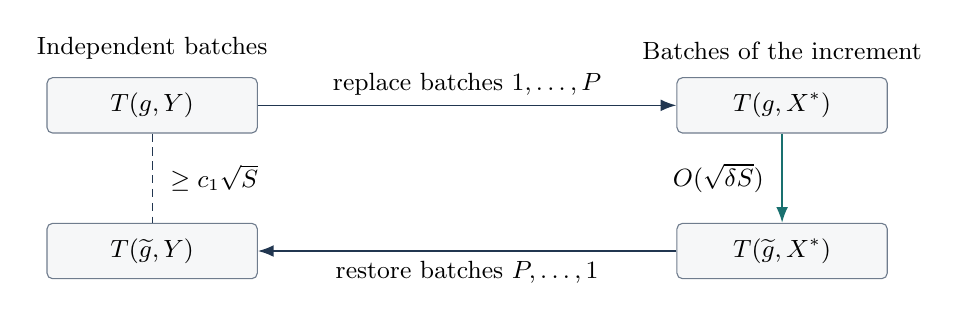
\begin{tikzpicture}[font=\small,
  state/.style={draw=ink!65,fill=ink!4,rounded corners=2pt,
    minimum height=20pt,minimum width=76pt,inner sep=3pt},
  path step/.style={-{Latex[length=2mm]},draw=ink,semithick}]
\node[state] (a) at (0,0) {$T(g,Y)$};
\node[state] (b) at (8.0,0) {$T(g,X^*)$};
\node[state] (c) at (8.0,-1.85) {$T(\widetilde g,X^*)$};
\node[state] (d) at (0,-1.85) {$T(\widetilde g,Y)$};
\node[above=3pt of a] {Independent batches};
\node[above=3pt of b] {Batches of the increment};
\draw[path step] (a.east) -- node[above]{replace batches \(1,\ldots,P\)} (b.west);
\draw[path step,draw=sea] (b.south) -- node[left=3pt]{\(O(\sqrt{\delta S})\)} (c.north);
\draw[path step] (c.west) -- node[below]{restore batches \(P,\ldots,1\)} (d.east);
\draw[densely dashed,draw=ink] (a.south) -- node[right=3pt]{\(\ge c_1\sqrt S\)} (d.north);
\end{tikzpicture}
\caption{The same lamp increment \(\widetilde g=g+e_jX_1\) with two
choices of reports. The vertical labels give root-mean-square distances.
The dashed segment compares the endpoints of the three-step detour.
With the increment's own batches in place, the middle step uses the
short list with high probability.}
\label{lamp:fig-path}
\end{figure}

Let \(J\) be the supremum of the root-mean-square separation in
Lemma~\ref{lamp:lemma} under its stated distance bounds, with \(C\)
chosen sufficiently large in terms of \(K_\delta\).
We claim that the root-mean-square cost of replacing batch \(a\) is at most
\begin{equation}\label{lamp:path-estimate}
 \sqrt{r_a\log(1/\delta)}\,J+\exp(-c''_\delta r).
\end{equation}
First average over layouts \(\ell_P,\ldots,\ell_a\), holding the
earlier layouts fixed. The points for \(Y^{(a-1)}\) and \(Y^{(a)}\)
depend on \(X_1,\ldots,X_{a-1}\) only through their common prefix
reports. The unaltered \(Y_a,\ldots,Y_P\) are independent
of the entire hash chain. By the joint law above, in the
expectation of this squared distance we can replace \(X_a\) by a fresh
independent uniform batch and use independent prefix reports, with
error \(O(S\exp(-c'_\delta r))\), since all the points concerned lie in a
ball of radius \(\sqrt S\) at the same reference state. This estimate
averages over prefix reports and requires no estimate conditioned on
one specified report value.

Apply Equation~\eqref{lamp:exchange} to the two independent words at batch \(a\).
Fix the other letters and the prefix reports. Immediately before the
average over \(\ell_a\), the letter in question affects only the bit
read by \(b_{\ell_a}\). If this position is ignored by that layout, the
two choices give the same point. At each layout the two points are at
distance at most \(\sqrt{\log(1/\delta)}\), by the flip move and coupling
all subsequent layouts. Over all layouts these points have diameter
at most \(\sqrt r\), by a one-batch reset with that same coupling.
After rescaling by \(1/\sqrt{\log(1/\delta)}\), their averages over
\(\ell_a\) are precisely a test for \(J\). Each summand in
Equation~\eqref{lamp:exchange} is thus at most \(J^2\log(1/\delta)\).
Completing the outer barycenters contracts the mean square. Taking
square roots and absorbing polynomial factors into the exponential
gives Equation~\eqref{lamp:path-estimate}. On the return path the translated
array is again uniform independently of all batches, since \(g\) was
independent uniform.

Sum the replacement lengths along both horizontal paths in
Figure~\ref{lamp:fig-path}. The \(L^2\) triangle inequality gives
\[
 c_1\sqrt S\le
 2J\sqrt{\log(1/\delta)}\sum_a\sqrt{r_a}
 +\sqrt{\delta S+S\exp(-c'_\delta r)}
 +2P\exp(-c''_\delta r).
\]
Choose \(\delta\) sufficiently small compared with \(c_1^2\), and then
\(K_\delta\) sufficiently large. Since \(\sum_a\sqrt{r_a}\le C m\sqrt r\)
and \(S=rm\), this gives \(J\ge c/\sqrt m\). Choosing a placement
within a factor two of the supremum proves Lemma~\ref{lamp:lemma}.

\subsection{From barycenters to directions}

\begin{proof}[Proof of Theorem~\ref{lamp:certificate}]
We first normalize the mean squared row norm to one. Given a distribution
on layouts, take the points of Lemma~\ref{lamp:lemma}, put
\(p=\operatorname{bar}_i u_i\), and set
\(\sigma^2=n^{-1}\sum_i d(p,u_i)^2\). The triangle inequality gives
\(\sigma\ge c/(2\sqrt m)\). In the completed tangent cone at \(p\) take
\[
 x_i=\log_p(u_i)/\sigma,\qquad Z_{\ell,v}=\log_p(z_{\ell,v}).
\]
To realize the tangent cone in \(\mathcal M\), rescale distances
by integers \(k\to\infty\). Represent a direction of length \(t\)
by the points at distance \(t/k\) on its geodesic. In a pointed
ultralimit this is an isometric embedding and extends to the
completed cone. Its image is closed and convex. The logarithm map preserves distance to \(p\)
as norm and contracts pairwise distances. First variation of the mean
squared distance at its minimizer shows that
\(\sum_i\langle v,\log_p u_i\rangle\le0\) for each represented direction,
and hence for every tangent vector by continuity. Thus the \(x_i\)
have barycenter zero \cite{BH,Sturm}. The bounds on the \(Z\)'s follow
from contraction and from the diameter bound on the convex hull of
the original points, which contains \(p\).

Use the variance inequality for the measure with barycenter \(u_i\),
evaluated at \(p\). It gives
\[
 \mathbb E_\ell d(p,z_{\ell,b_\ell(i)})^2
 \ge d(p,u_i)^2+\mathbb E_\ell d(u_i,z_{\ell,b_\ell(i)})^2 .
\]
On expanding the cone pairing and using contraction, we obtain
\(\mathbb E_\ell\langle x_i,Z_{\ell,b_\ell(i)}\rangle
\ge d(p,u_i)^2/\sigma\). The total expected score is therefore at
least \(n\sigma\). Write \(s_\ell=\sum_i\langle x_i,Z_{\ell,b_\ell(i)}\rangle\) for
the score at layout \(\ell\). For every distribution \(q\) there is
now a configuration with \(\sum_\ell q_\ell s_\ell\ge cn/\sqrt m\).
For each configuration the strict inequality
\(\sum_\ell q_\ell s_\ell>cn/(2\sqrt m)\) defines an open set of
distributions. These sets cover the compact simplex. A finite subcover
gives a finite matrix, with configurations as rows, layouts as columns,
and the scores as entries. Minimax gives a convex combination of its
rows with score at least \(cn/(2\sqrt m)\) in every column. Realize this combination by
an \(\ell_2\) product, multiplying the vectors in each factor by the
square root of its weight. All metric bounds and the normalization
survive, and barycenters in the product are coordinatewise.

Finally enlarge the original list to include every cyclic translate
\(i\mapsto b_\ell(i+t)\) of every layout, with indices modulo \(n\).
Apply the preceding construction to the enlarged list, indexing each
layout by \((\ell,t)\). In the product of \(n\) copies take the rows
\(n^{-1/2}(x_{i+t})_t\) and centers
\(n^{-1/2}(Z_{(\ell,-t),v})_t\). At row \(i+t\) layout
\((\ell,-t)\) reads the original bit \(b_\ell(i)\). Thus the row
at position \(i\) has squared norm \(n^{-1}\sum_k\|x_k\|^2=1\).
The product rows are centered and each layout keeps its score bound. The enlarged list has at most \(nL\) members,
so \(m+\log(nL)\le2(m+\log L)\) preserves the radius estimate.
\end{proof}

\section{Exterior tensors at a prescribed placement}\label{sec:exterior}

The star centered at the cone tip supplies a tensor by sending its
indices separately to their sites. To detect the saving obtained by
using a separate supplier on each side of a balanced cut, we need a
tensor whose price at the original sites is already close to the cost
of the star. We first construct such a tensor for a prescribed
placement. In one copy, its nonzero entries are maximal minors of a
matrix selected for those sites and their spectral price.
Section~\ref{sec:packing} will group copies by site and retain certain
row letters to obtain a weighted tensor by restriction from one
explicit binary tensor.

Let $Y$ be a complete Hadamard cone with tip $0$ and homogeneous spectral
prices over an algebraically closed field $K$. We use natural logarithms.
For a $b\times N$ matrix $C$, consider $N$ inputs with two states,
empty and occupied. The coefficient on the set of occupied inputs $I$
is the ordered minor $\det C_I$ when $|I|=b$, and zero otherwise.
For example, when the columns are $(1,t_i)^{\mathsf T}$ and $b=2$,
the coefficient on $\{i,j\}$, $i<j$, is $t_j-t_i$. The exterior
product of the occupied columns produces these coefficients and lets
us keep track of the number of times each input is used in many copies.

More generally, let $A_i\subseteq E$ be subspaces spanning a
finite-dimensional space $E$. For $\ell\ge1$, wedge the inputs from
$\bigwedge^*(A_i\otimes K^\ell)$ in a fixed order, take the component
of top degree, and apply a volume form on $E\otimes K^\ell$. Write
$\Omega_\ell((A_i))$ for this multilinear form. Its \emph{sector}
$\Omega_{\ell,p}$ fixes the exterior degree $p_i$ at each input, with
$\sum_i p_i=\ell\dim E$. A \emph{supplier} $(A_i,y_i,\theta_i)$ puts
this input at the site $y_i$ and credits it $\theta_i$ units per degree.
The value of a list of suppliers is the largest biased sector price per
copy, optimized over the number of copies,
\begin{equation}\label{ext:value}
 \lambda((A_i,y_i,\theta_i)_i)
 =\sup_{\ell\ge1}\frac1\ell
   \max_p\left\{H(\Omega_{\ell,p};y)+\sum_i\theta_i p_i\right\}.
\end{equation}
Linear maps into $E$ may replace the inclusions $A_i\subseteq E$.
Factoring a map through its image and choosing a linear section gives
restrictions in both directions, so the sector prices agree. Taking
one map $K\to E$ per column of $C$ gives the form $\Omega_\ell(C)$
and the value $\lambda(C;y,\theta)$.

A column of degree $p$ in $\ell$ copies has local dimension
$\binom{\ell}{p}$. Sending this input from the tip to a site at
distance $r$ costs at most $r\log\binom{\ell}{p}$. If $h$ denotes
binary entropy in nats, its biased price per copy is bounded by
$rh(p/\ell)+\theta p/\ell$. Maximizing the latter over $p/\ell\in[0,1]$
gives the budget for a single column,
\[
 A(r,t)=r\log(1+e^{t/r})\quad(r>0),\qquad
 A(0,t)=\max(0,t),
\]
where $t$ is its bias. Summing these budgets gives the star upper bound
$\lambda(C;y,\theta)\le\sum_i A(\|y_i\|,\theta_i)$.
We use Vandermonde matrices with columns
$(1,t_i,\ldots,t_i^{b-1})^{\mathsf T}$ for distinct $t_i\in K$.
Any $b$ of these columns form a basis of $K^b$.

\begin{theorem}[Exterior near-star estimate]\leavevmode\phantomsection\label{ext:star}
Let $x_1,\ldots,x_d$ be unit sites with uniform Cartan barycenter $0$.
Give each site $q$ column suppliers, with identical lists of biases
\[
 \theta_j=-M+(2j-1)M/q,\qquad 1\le j\le q.
\]
Suppose $N=dq$ is even and $M\ge100\log N$. Write $y,\theta$ for
the resulting lists of $N$ sites and biases. There exists an
$(N/2)\times N$ Vandermonde matrix $C$ satisfying
\[
 0\le \sum_i A(1,\theta_i)-\lambda(C;y,\theta)
       \le C_0 M(1+N/q^2)\log N
\]
with an absolute constant $C_0$.
\end{theorem}

To see what the lower bound asks of the columns, give the tip an
additional supplier of the whole space $E$ and vary its bias $s$.
As $s$ increases, it becomes advantageous to take more degrees at
the tip. The marginal value of $s$ measures those degrees per copy.
Subtracting it from $b=\dim E$ gives the \emph{threshold rank} $r_s$
still supplied by the original columns. Equation~\eqref{ext:recover}
will recover the original price by integrating $r_s$.

A single column at a unit site has threshold rank
$p_i(s)=(1+e^{s-\theta_i})^{-1}$, and
$\int_0^\infty p_i(s)\,ds=A(1,\theta_i)$. To recover the star budget
we would like $r_s$ to be close to $\sum_i p_i(s)$ above zero, where
the columns must contribute independently, and close to $b$ below
zero, where they must fill $E$. For an ordinary subset of Vandermonde
columns these two requirements meet in the identity
$\rank(C_I)=\min(b,|I|)$.

For priced columns we can construct an event of dimension $p_i(s)$ for
each column. Intersection dimensions give a probability law for each
\emph{pair} of events. These laws need not extend to a joint law for all
the events, so in general we cannot sample a subset $I$ and count its
members. Section~\ref{sec:flags} inserts event indicators one at a
time and shows how the resulting count bounds the Vandermonde rank from
below.
Section~\ref{sec:achieve} uses the centered sites and the evenly spaced
biases to control the second moment of this count over insertion orders.
This gives one choice of columns with small integrated rank loss.

\subsection{Exterior price rules}

We record the properties of the exterior value that underlie the
threshold rank. First, the supremum in~\eqref{ext:value} is a limit.
Split the copy indices into blocks of lengths $\ell_1,\ell_2$ and fix
a maximizing sector in each block. Wedge the two inputs locally at
every supplier. The sector of the combined system then restricts to
the product of the two sectors. The sign for moving the blocks past
one another is constant on the fixed degrees. Hence the unnormalized
maxima are superadditive. They are bounded above by $O(\ell)$ by
transport, and spanning gives a nonzero sector. Fekete's lemma now
yields the limit. Reordering suppliers also changes each sector only
by a scalar sign. For the full exterior form this sign can depend on
the degrees of the inputs.

Enlarging or adding suppliers gives restrictions onto the original
sectors. Increasing a bias can only increase the value, and shifting all biases
by $a$ adds $a\dim E$ because the total degree is fixed. Joint convexity
and positive homogeneity in the labels follow from the corresponding
properties of price. Continuity follows from transport and the bound
$\ell\dim A_i\log 2$ on the logarithm of each local dimension. A zero
subspace contributes nothing.

Two suppliers at the same site and bias may be merged by replacing their
subspaces with their sum. Precomposing the merged form with local
wedge multiplication gives the form on each split sector. For the reverse inequality, fix a
merged degree and take the direct sum of the wedge maps over all degree
splits. This map is onto because the two subspaces span their sum. A
linear section expresses the merged tensor as an ordinary sum of
restrictions, one for each of at most $\ell\dim E+1$ splits. Their
bias credits agree. Lemma~\ref{price:rules} bounds the extra price by
$O(\log(\ell+1))$, which vanishes per copy. Direct sums of systems in
complementary summands of $E$ add values, since their nonzero sectors
factor.

Finally, consider lists $L_1,L_2$ with a spanning common sublist.
We prove the diminishing-increments inequality
\[
 \lambda(L_1\cup L_2)+\lambda(L_1\cap L_2)
 \le \lambda(L_1)+\lambda(L_2).
\]
Place the lists in separate summands of $E\oplus E$ and merge common
suppliers. For $t\ne0$ apply the change of coordinates
$(u,v)\mapsto(u+v,tv)$. Each common supplier still supplies
$A_i\oplus A_i$ and can keep its original basis. Use the transformed
bases, polynomial in $t$, for all exclusive suppliers. At $t=0$ they
supply subspaces of the first summand. Each limiting sector is thus
a specialization of isomorphic sectors, so its price cannot increase
by Lemma~\ref{price:rules}. Splitting the common suppliers again gives
the union in the first summand and the intersection in the second.
Additivity now gives the displayed inequality. For lists with repeated
members, use named occurrences to form the union and intersection.

\section{From prices to flags}\label{sec:flags}

Theorem~\ref{ext:star} asks for a matrix whose columns nearly attain
their combined star bound. At the tip, a bias threshold selects ordinary
subspaces, and the dimension of their span records how much of the
ambient space they supply. Away from the tip the same measurement,
obtained from the exterior price, can take fractional values. We need
to estimate it for many columns at once.

We first recover a dimension for sums, intersections, and images of
formal subspaces from these threshold measurements. The subspaces for
one site, ordered by bias, then form a flag. Intersecting the levels of
two flags gives them a pair law. Successively combining pairs of flags
will provide a count of the columns available at a threshold.
Lemma~\ref{flag:insertion} gives a lower bound on the rank of
Vandermonde columns by the expected count truncated at the number of
rows, up to arbitrarily small error. One matrix realizes this bound
at any prescribed finite set of thresholds.

\subsection{Threshold rank}

Let $Y$ be a Hadamard cone with tip $0$, and let $K$ be an infinite field.
A \emph{supplier} in a finite-dimensional $K$-space $E$ is a triple
$(A,y,\theta)$ with $A\subseteq E$ a subspace, $y\in Y$ a site and
$\theta\in\mathbb R$ a bias. Call $(y,\theta)$ its label. A list spans if
its supplied subspaces span $E$.
The exterior value in~\eqref{ext:value} assigns a finite number
$\lambda_E(L)$ to each spanning list $L$. In this section we may use
any such value with the following properties.
\begin{enumerate}
\item Isomorphisms of $E$ and permutations of the list preserve value.
The value is continuous in the labels, positively homogeneous under their
common dilation, and convex under simultaneous geodesic interpolation
of sites and linear interpolation of biases.
\item Increasing a bias, enlarging a subspace or adding a supplier can
only increase value. Shifting every bias by $t$ adds $t\dim E$.
Suppliers with the same site and bias merge by summing their subspaces,
and supplying the zero space has no effect.
\item Taking the direct sum of two spaces with their respective suppliers
adds their values. Adding a supplier has diminishing increments under
enlargement of a spanning base list.
\end{enumerate}
Section~\ref{sec:exterior} established these properties for the exterior
value. A supplier is redundant if another supplier at the same site
offers a containing subspace at a higher or equal bias. Indeed, raising
the first bias to the second allows the two suppliers to merge, and
monotonicity gives equality at the original bias.

For any list $L$ in $E$, append the \emph{root supplier} $(E,0,s)$ and
write $\lambda_L(s)$ for the value of the resulting spanning list. The
root offers all of $E$. Its marginal value measures how much dimension
it supplies at bias $s$. The remainder is the \emph{threshold rank}
of the ordinary suppliers. Writing $L-s$ for the list with $s$
subtracted from every ordinary bias, we have
\begin{equation}\label{flag:capdef}
 r_E(L)=\dim E-\lambda'_{L,+}(0),\qquad
 r_E(L-s)=\dim E-\lambda'_{L,+}(s).
\end{equation}
The second identity follows by translating all biases. Convexity
ensures the existence of the right derivative. Monotonicity and bias
translation bound it between zero and $\dim E$.

\begin{lemma}[Threshold rank]\label{flag:capacity}
The rank $r_E$ takes values in $[0,\dim E]$, adds on direct sums, and is
unchanged on merging equal labels or adding unused ambient dimensions.
It is monotone under adding suppliers, enlarging subspaces and increasing
biases. It is unchanged by independent positive dilations of the labels
and has diminishing increments under adjoining suppliers to any list.
\end{lemma}

\begin{proof}
For the empty list the root has value $s\dim E$ by homogeneity and
translation. The direct sum and merging rules pass through the derivative
(the root of a direct sum can itself be split at its label).
For $h>0$, raising the root bias from $0$ to $h$ amounts to adding
$(E,0,h)$. Its increment can only decrease when $L$ grows. Passing to
the right derivative proves monotonicity under adjoining a supplier.
An enlargement or a bias increase amounts to adjoining the improved
supplier.

Common dilation of the labels preserves rank by homogeneity. For
$0<t<1$, adjoin a shortened copy $u_t=(A,ty,t\theta)$ of an existing
supplier $u=(A,y,\theta)$. At every root bias $s\ge0$, the root
absorbs $u_0$ and the original supplier absorbs $u_1$. By convexity
along this segment and monotonicity under addition, $u_t$ also leaves
the value unchanged. Deleting $u$ can only decrease rank, so replacing
$u$ by $u_t$ can only decrease rank. Dilate the resulting list by
$1/t$ and shorten each of its other labels by $t$ to return to the
original list. This proves equality for one shortened label and hence
invariance under arbitrary independent positive dilations.

It remains to compare the rank gained by adjoining $u$ to two lists
$L\subseteq L'$. Shorten $u$ towards the root. The added rank stays
constant by dilation invariance, and in the limit it can be read from
the derivative in the bias of the shortened supplier.

To justify the derivative calculation, perturb the ordinary biases,
keeping shared occurrences identical. For almost every perturbation,
the root-augmented values for $L,L'$ and for their augmentations by
$u_{1/k}$, $k\ge1$, are all differentiable in their biases at root bias
zero. Indeed each finite convex value is differentiable almost
everywhere. Bias translation determines it from its restriction to
root bias zero, and scaling the additional bias by $1/k$ is an
invertible coordinate change. We may therefore make this countable
family of choices simultaneously.

At a differentiability point the sum of the ordinary suppliers' bias
derivatives equals the rank. Apply this to $L$ augmented by $u_{1/k}$,
differentiating in the actual bias of that supplier. As $k\to\infty$,
the derivatives at the old suppliers converge to those for $L$ alone.
In fact, as convex functions of the old biases the values converge
pointwise by continuity and redundancy of $u_0$. Left and right
difference quotients squeeze each partial derivative at a point of
differentiability of the limit. Independent dilation leaves the
augmented rank fixed. The bias derivative at $u_{1/k}$ therefore
converges to $r_E(L\cup\{u\})-r_E(L)$.
For every $k$ that derivative can only decrease on passing from $L$ to
$L'$, since raising the bias is equivalent to adding a supplier and
$\lambda$ has diminishing increments. This proves the desired comparison
at the perturbed biases. Finally approximate all ordinary biases
simultaneously from below. Monotonicity squeezes each perturbed rank
between its original value and its value after a common negative shift.
The latter converges to the original value by right continuity of the
right derivative in \eqref{flag:capdef}.
\end{proof}

When all suppliers lie at the tip, the threshold rank is
\[
 r_E(L-s)=\dim\!\sum_{\theta_i>s} A_i .
\]
After the shift by $s$, the root absorbs every supplier of nonpositive
bias as its own bias increases from zero. Independently dilating the
remaining labels to $(0,1)$ merges their subspaces into a single space
$A$. On $A$ the root is redundant for small positive root bias. On a
complement it is the sole supplier. This accounts for both the rank
formula and the strict inequality at a bias tie.

A single column illustrates what changes away from the tip. For the
exterior price, let $E=K$ and put the column at a site of radius $u>0$
with bias $\theta$. The two-supplier exterior pairing, computed below,
gives $\lambda_L(s)=s+u\log(1+e^{(\theta-s)/u})$. Thus
$r_E(L-s)=(1+e^{(s-\theta)/u})^{-1}$. At the bias tie the column
supplies half a dimension. To combine such fractional contributions
we need a dimension calculus that can also measure their overlaps.

\subsection{Dimension of subspace expressions}

Introduce a formal space $X$ of normalized dimension one and a symbol
$U_j$ for the subspace supplied by label $j$. The unrestricted label $(0,1)$
designates $X$ itself. At that label a supplier of $A$ has rank
$\dim A$ by the tip calculation. For a scalar matrix $B$ with labeled
columns write $r(B)$ for the threshold rank in its output space, using
one supplier per label with subspace the span of its columns.

Consider a variable $v_i\in U_{j_i}$ for each input column. Given
scalar matrices $P,Q$ over $K$ with those columns, form the expression
in $X^e$
\[
 T=\{Pv: Qv=0,\ v_i\in U_{j_i}\},
\]
where $e$ is the number of rows of $P$. It describes the outputs $Pv$
left after imposing the constraints $Qv=0$. Sums, intersections,
direct sums, and scalar images each admit such a description by
introducing variables and linear constraints. In module theory these
are positive primitive subspace expressions \cite{Prest}. An inclusion
between two expressions is \emph{universal} if it holds for every
substitution of an actual vector space for $X$ and actual subspaces for
the $U_j$, with the unrestricted label interpreted as the whole space.

For ordinary subspaces, projecting the joint image $(Pv,Qv)$ to $Qv$
has kernel isomorphic to $T$. The proposition shows that the difference
of the corresponding threshold ranks also defines a dimension and
satisfies the same rank--nullity identity.

\begin{proposition}[Dimension calculus]\label{flag:dimension}
The formula
\begin{equation}\label{flag:ppdim}
 \dim_*T=r\!\binom{P}{Q}-r(Q)
\end{equation}
is nonnegative, respects universal inclusions and adds on direct sums.
For any scalar map $M$,
\[
 \dim_*T=\dim_*M(T)+\dim_*(T\cap\ker M).
\]
In particular $r_E(L)=\dim_*\big(\sum_i A_i\otimes U_{j_i}\big)$, where
each summand denotes the image along a basis of $A_i$ of independent
variables with label $j_i$.
\end{proposition}

\begin{proof}
First consider adding unrestricted columns spanning a space $D$ to a
matrix $B$. The resulting rank is
\[
 \dim D+r(B\bmod D).
\]
Indeed, the unrestricted columns supply the full rank $\dim D$ on $D$.
Copies of those columns with any other label add zero rank there. By
invariance under unused ambient dimensions and diminishing increments
(Lemma~\ref{flag:capacity}), they still add zero rank in the presence of
$B$. Make these copies for every label of $B$. Within each label we can
now subtract components in $D$ from its columns while preserving their
span together with the copies. The remaining columns lie in a fixed
complement of $D$. Removing the copies and applying direct sum
additivity gives the formula.

For $B=\binom{P}{Q}$ take $D=K^e$ in the first output coordinates. The
gain from adding the unrestricted columns of $D$ is $e-\dim_*T$. It
lies in $[0,e]$ and can only decrease on adjoining more input columns.
Thus $\dim_*T$ is nonnegative and can only increase with more inputs.
Dropping constraint rows also increases this dimension. For each
dropped row adjoin an unrestricted column on its constraint axis to
the joint matrix. By the quotient formula, that axis contributes one
to both ranks in~\eqref{flag:ppdim}, leaving exactly the expression
with the row dropped.

Now suppose $T\subseteq T'$ universally, with respective data
$(P,Q)$ and $(P',Q')$. We need a scalar comparison between their
presentations. If $T$ has $s$ inputs, substitute
\[
 X=K^s/\operatorname{rowspan}(Q)
\]
and let $v_i$ be the classes of the standard basis vectors. For each
restricted label take $U_j$ to be spanned by its $v_i$. This choice
realizes $Qv=0$ and imposes exactly the row relations generated by
$Q$. Universal inclusion gives $v'$ of the allowed labels with
$P'v'=Pv$ and $Q'v'=0$. Expressing $v'$ in the generators $v_i$
produces a scalar matrix $A$. Each restricted row uses only columns
of its own label, and an unrestricted row may use any column. The
relations yield scalar matrices $J,J'$ with
\[
 P'A-P=JQ,\qquad Q'A=J'Q.
\]

Row operations therefore let us replace $P$ by $P'A$ and append the
redundant constraints $Q'Av=0$ in~\eqref{flag:ppdim}. Drop the old
constraints $Qv=0$, increasing dimension. The resulting joint matrix
is $\binom{P'}{Q'}A$. Each of its labeled columns lies in the span of
columns of $\binom{P'}{Q'}$ with that label and of unrestricted
columns. Copy the unrestricted columns into each label. These copies
contribute zero in both ranks by the quotient argument above. Enlarging
the column spans now gives $\dim_*T\le\dim_*T'$. Two presentations of
the same expression include each other universally, so their dimensions
agree.

Direct sums add by Lemma~\ref{flag:capacity}. The dimension of $M(T)$ is
$r\binom{MP}{Q}-r(Q)$. For $T\cap\ker M$ the added equations are $MPv=0$,
so the two dimension formulas telescope, since stacking $MP$ with $P,Q$
does not change their joint rank. Taking $Q$ to have no rows gives the
last assertion.
\end{proof}

Apply the kernel identity to addition on $U\oplus V$. Its kernel is a
scalar copy of $U\cap V$, so
\begin{equation}\label{flag:modular}
 \dim_* (U+V)+\dim_*(U\cap V)=\dim_*U+\dim_*V .
\end{equation}
We identify expressions $U,V$ if $U\cap V$ and $U+V$ have the same
dimension. For nested expressions of equal dimension, adjoining a
third expression by sum or intersection preserves equality of
dimension by \eqref{flag:modular}. The same holds for direct sums and
scalar images by Proposition~\ref{flag:dimension}. These observations,
applied through $U+V$, give transitivity and allow equivalent expressions
to be substituted in subsequent linear constructions.
Now specialize to the subspace symbols of a single site $y$. If
$\theta\le\theta'$, adding the lower-bias supplier to the higher one
leaves its rank unchanged. Thus $U_{y,\theta}+U_{y,\theta'}$ is
equivalent to $U_{y,\theta'}$. For any finite list of biases their
cumulative sums give universally nested representatives. Likewise,
in the pair of labels $(y,\theta),(ty,t\theta)$ we can dilate one
label until they agree and merge the pair. Its sum then has the same
dimension as each member. Hence $U_{ty,t\theta}$ and $U_{y,\theta}$
are equivalent for every $t>0$.

\subsection{The metric on flags}

An \emph{event} is a subspace expression in $X$, with its dimension
in $[0,1]$ interpreted as a probability. A finite flag $F$ is a
decreasing filtration of $X$ by such expressions, with finitely many
real jump levels. Its thresholds $F_{\ge a}$ range from $X$ to zero.
We take them to be universally nested, using cumulative sums when they
are initially nested only up to equivalence. Their dimensions are the
upper tails of a probability law on the levels. Two flags $F,G$ also
have a pair law, determined by
\begin{equation}\label{flag:pair}
 \Pr(F\ge a,G\ge b)=\dim_*(F_{\ge a}\cap G_{\ge b}).
\end{equation}
Indeed a cell mass is a successive difference of four intersection
dimensions. The intersection for the two weaker thresholds contains the
sum of the intersections obtained by strengthening either threshold.
Equation~\eqref{flag:modular} then gives nonnegativity.

A family of these pair laws may fail to admit a common probability
space. For example, take three distinct lines in a two-dimensional
space and normalize dimension by $1/2$. Each line has probability
$1/2$, while each pair has intersection probability zero. Three events
with these probabilities would have union probability $3/2$. We
therefore combine many events one pair at a time.

For a fixed pair, the grid of its jump levels has more structure.
For each upper set $S$ in this grid, let $U_S$ be the sum of the
intersections $F_{\ge a}\cap G_{\ge b}$ indexed by the minimal
elements $(a,b)$ of $S$. Unions correspond to sums and intersections
to intersections. These identities hold universally because for every
actual substitution the two filtrations admit a common adapted basis.
To construct one, work from the deeper grid intersections upwards.
Extend the bases already chosen for the two immediately deeper
intersections, whose common basis was fixed at the doubly deeper
intersection. Each $U_S$ is then a coordinate subspace in this basis.
Modularity and~\eqref{flag:pair} give
$\dim_*U_S=\Pr((F,G)\in S)$.

In particular, the upper level sets of a coordinatewise nondecreasing
function $f$ give a flag $f(F,G)$. Its law is the pushforward of the
pair law. The same grid gives the joint law of any two such functions
of $F,G$. This permits interpolation between two flags even when a
third flag has no joint law with them.

We use the notation
\[
 \langle F,G\rangle=\mathbb E[FG],\qquad
 \|F\|^2=\mathbb E[F^2],\qquad d(F,G)^2=\mathbb E[(F-G)^2],
\]
where each expectation uses the indicated law. The metric estimate
below will control what happens during insertion when one indicator is
changed. For the CAT(0) metric on filtrations of modular lattices of
finite length, see \cite[Proposition~2.6]{Cornut}.

\begin{proposition}[Flag metric]\label{flag:metric}
After identification at distance zero, finite flags have a CAT(0)
metric, with geodesic $H_t=((1-t)F+tG)$ defined by the two-flag
construction. The completion is Hadamard. Positive dilation is a
homothety. For fixed $Q$ the pairing with $Q$ is $\|Q\|$-Lipschitz.
\end{proposition}

\begin{proof}
The two-flag grid gives distances along the candidate geodesic
$H_t$. To compare it with a third flag $Q$ we first take
$Q=1_A$, the indicator flag of an event $A$. For each upper set $S$
of the $F,G$ grid put $w(S)=\dim_*(A\cap U_S)$. This function is
supermodular because the sum of two intersections with $A$ lies in
the intersection of $A$ with the sum. More explicitly, modularity
gives
\[
 w(S)+w(T)\le w(S\cup T)+w(S\cap T).
\]
Order the grid points $p_1,\ldots,p_s$ so each initial segment $S_i$
is upper, and set $S_0=\varnothing$. For coordinatewise nondecreasing
$f$, the expectation $\langle Q,f(F,G)\rangle$ equals
\[
 \min_{(p_i)}\ \sum_{i=1}^s f(p_i)\big(w(S_i)-w(S_{i-1})\big).
\]
Indeed the pair law gives equality for a decreasing order of $f$.
From any allowed order, swapping adjacent points inverted by $f$
preserves the upper-set condition, since those points are incomparable.
Supermodularity shows that such a swap can only decrease the sum.
The minimum is concave in $f$. Every finite $Q$ decomposes as a constant
plus a nonnegative combination of its threshold indicators, with the
corresponding equality of pairings. For every $Q$ this proves
\[
 \langle Q,H_t\rangle\ge(1-t)\langle Q,F\rangle+t\langle Q,G\rangle.
\]
Computing $\|H_t\|^2$ in the pair law and expanding now yields
\[
 d(Q,H_t)^2\le (1-t)d(Q,F)^2+t d(Q,G)^2-t(1-t)d(F,G)^2 .
\]
Nonnegativity of the left side, with
$t=d(Q,F)/(d(Q,F)+d(Q,G))$, gives the triangle inequality
(the zero-denominator case follows at $t=1/2$).
The joint law on the grid gives
$d(H_t,H_u)=|t-u|d(F,G)$, establishing the geodesic and CAT(0)
comparison. Dilation and homogeneity of the pairing follow from the
pair laws. Finally the triangle inequality gives
$|d(F,aQ)-d(G,aQ)|\le d(F,G)$ for $a>0$.
Taking the difference of squares and dividing by $2a$, then letting
$a\to\infty$, shows
$|\langle F,Q\rangle-\langle G,Q\rangle|\le\|Q\|d(F,G)$.
All these properties pass to the metric completion.
\end{proof}

The exterior application has strict thresholds at every real level.
Suppose a decreasing family $F_{>a}$ has dimensions equal to the
tails of a probability law of finite second moment. Truncate and
discretize the levels, using nested representatives at each finite
set of thresholds. Two such approximations can be coupled on their
combined chain. Their distance is the ordinary $L^2$ distance of the
two discretizations under the given law, so they converge in the flag
completion. For two families the pair upper tails are still the
dimensions of the threshold intersections. Indeed, by
\eqref{flag:modular} the change in an intersection dimension on
changing one threshold is bounded by the change in its marginal. The
upper tails are therefore right-continuous, and the continuous pairing
is the integral of the product under this pair law.

For each site $y$ take $F(y)_{>a}=U_{y,-a}$. Increasing $a$ lowers
the bias and gives a decreasing family. Whenever its tail dimensions
have finite second moment as above, it defines a flag $F(y)$. The tip
calculation gives $F(0)=0$, and equivalence of dilated labels gives
$F(ty)=tF(y)$ for $t>0$. For the exterior value, the single-column
calculation will identify the law at every site.

\subsection{Insertion along a column curve}

Write $F+G$ for twice the midpoint of $F,G$. On their two-flag grid,
this is the flag of the function $(f,g)\mapsto f+g$. Shifting its
arguments shifts this sum by the total shift. CAT(0) convexity makes
addition $1$-Lipschitz in each argument. Given events $H_1,\ldots,H_N$
in a fixed order, start with $V_0=0$ and form
$V_i=V_{i-1}+1_{H_i}$. At each step the grid of the current flag and the next
indicator defines the new flag, and their pair law gives its
distribution. The final flag
$V=V_N$ is the \emph{insertion sum} for this order.

Write $D_j$ for the current threshold at level $j\ge1$, and put
$D_0=X$. After inserting an event $H$, the threshold becomes
\begin{equation}\label{flag:thresholdupdate}
 D_j^{\mathrm{new}}=D_j+(H\cap D_{j-1})\qquad (j\ge1).
\end{equation}
Indeed, the upper set for $V_{i-1}+1_H\ge j$ consists of the old
threshold together with the part of level $j-1$ that meets $H$. Thus
after two insertions the first two thresholds are the sum and the
intersection of the events. In general $V$ is nonnegative and
integer-valued. Its first $m$ threshold dimensions sum to
$\mathbb E\min(m,V)$, the count that can fit into $m$ row directions.
The next lemma realizes this quantity as a lower bound on column rank.

\begin{lemma}[Insertion along a curve]\label{flag:insertion}
Let $v(t)\in K(t)^m$ be regular at zero and suppose its Taylor
coefficient columns span $K^m$. Read the coefficients in order of
degree, retaining each that increases the span. Denote the retained
basis by $e_1,\ldots,e_m$. Let $D_j$ be the thresholds obtained by
inserting $H_1,\ldots,H_N$ in that order. For every subspace expression
$U\subseteq X^m$ and $\varepsilon>0$, there are parameters with
\[
 \dim_*\!\left(U+\sum_{i=1}^N v(t_i)H_i\right)
 \ \ge\ \dim_*\!\left(U+\sum_{j=1}^m e_jD_j\right)-\varepsilon .
\]
One tuple $(t_1,\ldots,t_N)\in K^N$ can meet finitely many such tests
with the same curve and insertion order, allowing the events and $U$
to vary between tests. It can be chosen in any specified nonempty
principal open subset of $K^N$, avoiding poles and pairwise
coincidences. For $v(t)=(1,t,\ldots,t^{m-1})^\top$ and $U=0$, the
lower bound is $\mathbb E\min(m,V)-\varepsilon$.
\end{lemma}


For the curve $(1,t,t^2)^\top$, suppose the earlier events have
supplied $e_1L_1+e_2L_2+e_3L_3$ with $L_1\supseteq L_2\supseteq L_3$.
At $t=0$ the new column supplies $H$ along $e_1$. On $H\cap L_1$
the old space $e_1L_1$ can cancel the constant term of the new column.
Dividing by $t$ exposes $e_2$ at zero. On $H\cap L_2$ the old spaces
can cancel both lower terms, exposing $e_3$ after division by $t^2$.
Specializing all three expressions together captures the three
contributions in~\eqref{flag:thresholdupdate}.

\begin{proof}
We first record a specialization estimate for the dimension of $B(t)T$,
where $T$ is any fixed subspace expression and $B$ is a polynomial
matrix of degree at most $b$. At $q>b$ distinct scalars $a_i$,
\begin{equation}\label{flag:special}
 \sum_{i=1}^q\dim_* B(a_i)T\ \ge\ (q-b)\dim_* B(0)T .
\end{equation}
Take independent inputs from $T$ as the $q-b$ coefficients of a vector
polynomial $p$ of degree less than $q-b$. Evaluating $B(t)p(t)$ at the
$a_i$ places the joint output in $\bigoplus_i B(a_i)T$.
Scalar interpolation recovers its coefficients since its degree is less
than $q$. Its first $q-b$ coefficients are a lower triangular block map
of the inputs with diagonal block $B(0)$. Its image has dimension at
least $(q-b)\dim_*B(0)T$. Project onto the first output, whose
dimension is $\dim_*B(0)T$. The kernel contains the image obtained
by setting the first input to zero, a triangular map of the same
form with one fewer input. Proposition~\ref{flag:dimension} now
adds the bounds for the image and kernel. This proves
\eqref{flag:special} by induction. If $R=\dim_* B(0)T$, a set of
$q>b$ parameters each losing at least $\eta>0$ satisfies
$q(R-\eta)\ge(q-b)R$, whence $q\le bR/\eta$. In particular all
but finitely many $a$ have $\dim_* B(a)T\ge R-\eta$.
Clearing common denominators gives the same conclusion for rational
maps regular at zero.

Let $L_j$ be the thresholds before the last insertion and put $L_0=X$.
Consider the expression
\[
 U+v(t)H_N+\sum_{j=1}^m e_j L_j .
\]
Write $v(t)=\sum_h c_h t^h$ at zero and $e_j=c_{h_j}$. For each $j$
add an independent input from $H_N\cap L_{j-1}$ along
\[
 w_j(t)=t^{-h_j}\!\left(v(t)-\sum_{h<h_j}c_h t^h\right).
\]
This is regular at zero with $w_j(0)=e_j$. Every coefficient of the
subtracted prefix lies in the span of $e_1,\ldots,e_{j-1}$. Since
$L_{j-1}\subseteq L_i$ for $i<j$, the extra inputs leave the image
unchanged away from zero and the poles. At zero they supply all the
new terms $e_j(H_N\cap L_{j-1})$ in \eqref{flag:thresholdupdate}.
Apply the specialization estimate to the direct sum of all the fixed
input expressions, including the new inputs. At zero its image contains
$U+\sum_j e_jD_j$ for the updated thresholds. At every nonzero regular
parameter the image equals the expression before the extra inputs were
added. For each test all but finitely many $t_N$ therefore attain the
required bound with slack $\varepsilon/N$.

Choose $t_N$ good for every test and such that the prescribed principal
open has a nonempty slice in the remaining variables. For the latter
condition it suffices to keep a nonzero coefficient of its defining
polynomial, viewed as a polynomial in those remaining variables,
nonzero at $t_N$. There are only finitely many excluded values and $K$
is infinite. For $N=1$ this choice proves the result. For $N>1$ apply
induction to the earlier insertions with fixed part $U+v(t_N)H_N$ and
the remaining slack. Distinctness and pole
avoidance can be included in the initial principal open. The case $N=0$
is immediate.
\end{proof}

\section{Approaching the star bound}\label{sec:achieve}

For a fixed placement of the columns, Theorem~\ref{ext:star} asks for a
matrix whose exterior price comes close to the sum of the individual wire
budgets. The rank calculus of Section~\ref{sec:flags} gives two ways to
measure what is lost. Above threshold zero we count column contributions
that become linearly dependent. Below zero we count dimensions that the
columns fail to supply. To turn these losses into a price, we first
recover the exterior value from its threshold ranks.

\subsection{Recovering price from threshold rank}

Let $L=((A_i,y_i,\theta_i))_i$ span $E$, and write $e=\dim E$.
Adjoin a supplier of all of $E$ at the tip with bias $s$, giving value
$\lambda_L(s)$. Write $r_s=r_E(L-s)$ for the rank after subtracting
$s$ from each original bias. By~\eqref{flag:capdef}, the right derivative of
$\lambda_L(s)$ is $e-r_s$. We claim that
\begin{equation}\label{ext:recover}
 \lambda(L)=\int_0^\infty r_s\,ds
             -\int_{-\infty}^0(e-r_s)\,ds .
\end{equation}
Indeed, at high bias the tip can supply all $e$ dimensions, giving
$\lambda_L(s)\ge se$. For an upper bound, transport the ordinary
inputs from the tip. If $a_i=\dim A_i>0$, the degree-$p_i$ input costs
at most $\|y_i\|\log\binom{\ell a_i}{p_i}$. Relative to supply entirely
from the tip, it also changes the bias term by $(\theta_i-s)p_i$.
Maximizing each contribution with the binary entropy bound gives
\[
 0\le\lambda_L(s)-se\le
 \sum_i a_i A(\|y_i\|,\theta_i-s)\longrightarrow0
 \qquad (s\to+\infty).
\]

At low bias the degree-zero tip input gives
$\lambda_L(s)\ge\lambda(L)$. To bound the gain from a tip input of
degree $p$, choose a basis of $E$ from the ordinary suppliers and
assign each basis vector to one containing supplier. In the induced
wedge basis of $E\otimes K^\ell$, the tip input has
$\binom{\ell e}{p}$ coordinates. For each coordinate, wedge its $p$
basis vectors into their assigned ordinary inputs and apply the
coordinate functional at the tip. This term is a restriction of an
ordinary sector. Its reordering sign is constant for the chosen
coordinate and input degrees. The tip contributes bias $ps$, while the
reassigned vectors contribute at least $-pT$ in the ordinary sector,
where $T=\max_i|\theta_i|$. Let $D$ be the diagonal rate of the sites
including the tip, and let $h$ denote binary entropy in nats.
By~\eqref{price:sum}, summing the coordinates costs at most
$D\log\binom{\ell e}{p}$. Hence, for $e>0$,
\[
 0\le\lambda_L(s)-\lambda(L)\le
 e\sup_{0\le u\le1}\{D h(u)+u(s+T)\}
 \longrightarrow0\qquad (s\to-\infty).
\]
Integrating the right derivative of the convex function $\lambda_L$
between these two limits gives~\eqref{ext:recover}. If $e=0$, both
sides vanish.

\subsection{Site flags and the barycenter}

At a site $y$ the threshold spaces $U_{y,-a}$ are nested as $a$
increases. We determine the law of the flag $F(y)$ with strict
thresholds $\{F(y)>a\}=U_{y,-a}$, beginning with $E=K$.
Two suppliers of $K$ at $y$ and the tip, with biases $t$ and $s$,
have value $s+A(\|y\|,t-s)$. Indeed, complementary exterior degrees
$p$ and $\ell-p$ give a perfect pairing of dimension $\binom{\ell}{p}$.
Its price is $\|y\|\log\binom{\ell}{p}$. Taking the entropy limit
and maximizing over $p/\ell$ gives the stated value. Now set $t=-a$.
Subtracting the right derivative at $s=0$ from one gives
\[
 \Pr_{\rm flag}\{F(y)>a\}=(1+\exp(a/\|y\|))^{-1}
 \qquad (\|y\|>0).
\]
Thus $F(y)$ has a logistic law of scale $\|y\|$ and mean zero.
At the tip the value is $\max(-a,s)$, giving the constant flag $F(0)=0$.
The finite second moments of these laws place the flags in the metric
completion of Proposition~\ref{flag:metric}.

The distance between two such flags also has an exterior interpretation.
Take suppliers at $y,z$ with biases $t_1,t_2$. At threshold $s$,
the rank of these suppliers of $K$ is the dimension of the sum of
their threshold spaces. By~\eqref{flag:modular} and~\eqref{flag:pair},
this is the upper tail at $s$ of $\max(F(y)+t_1,F(z)+t_2)$ in the
pair law of $F(y),F(z)$. Equation~\eqref{ext:recover} integrates this
tail to give the expectation of the maximum. On the other hand, the
perfect pairing at $y,z$ gives the value $t_2+A(d(y,z),t_1-t_2)$.
Writing $t=t_1-t_2$ and using $\mathbb E_{\rm flag}F(z)=0$, we obtain
\[
 \mathbb E_{\rm flag}\big(F(y)-F(z)+t\big)_+=A(d(y,z),t).
\]
The right derivative on the left is
$\Pr_{\rm flag}(F(y)-F(z)\ge-t)$. Thus the difference has a logistic
law of scale $d(y,z)$, with a point mass at zero when $y=z$.

The flag metric measures the second moment of this difference, so
$y\mapsto F(y)$ scales every distance by the standard deviation of a
standard logistic variable. Its image is closed by completeness of $Y$
and convex by uniqueness of geodesics in the CAT(0) flag space.
If $y_1,\ldots,y_N$ have barycenter at the tip, the sum of squared
distances to their flags is minimized at $F(0)=0$ within the image.
Projection onto the closed convex image can only decrease these
distances, so zero is also a minimizer in the full flag space.
For any flag $Q$ and $a>0$, comparison of this sum at $aQ$ and at
zero yields
$2a\sum_i\langle Q,F(y_i)\rangle\le Na^2\|Q\|^2$. Letting
$a\downarrow0$ gives
\begin{equation}\label{ext:center}
 \sum_{i=1}^N \langle Q,F(y_i)\rangle\le0
 \qquad\text{for every flag }Q .
\end{equation}
Each summand uses the pair law of $Q$ and the indicated site flag.

\subsection{Controlling lost rank by random insertion}

\begin{proof}[Proof of Theorem~\ref{ext:star}]
Write $b=N/2$. At threshold $s$ each slot $i$ supplies the event
$H_i(s)=\{F(y_i)>s-\theta_i\}$ of dimension
$p_i(s)=\Pr_{\rm flag}(H_i(s))$. For a Vandermonde matrix $C$, let
$r_s(C)$ be the rank of the image of $\bigoplus_i H_i(s)$ under its
column map. Since the sites are unit,
$\int_0^\infty p_i(s)\,ds=A(1,\theta_i)$. Equation~\eqref{ext:recover}
therefore expresses the star deficit exactly as
\[
 \sum_i A(1,\theta_i)-\lambda(C;y,\theta)
   =\int_0^\infty K_+(s)\,ds+\int_{-\infty}^0 K_-(s)\,ds ,
 \qquad
 \begin{aligned}
 K_+(s)&=\sum_i p_i(s)-r_s(C),\\
 K_-(s)&=b-r_s(C).
 \end{aligned}
\]
For $s\ge0$, $K_+$ measures the kernel dimension of the column map
and decreases as its domain shrinks. For $s\le0$, $K_-$ measures the
missing image dimension and decreases as $s$ moves left. Both lie in
$[0,N]$. It suffices to control them at finitely many thresholds for
a single choice of $C$.

\emph{Centering the indicators.}
For $|s|\le M/2$, put
\[
 c_s=\tfrac12-\tfrac{s}{2M},\qquad X_i(s)=\mathbf1_{H_i(s)}-c_s .
\]
The scalar $c_s$ is the fraction of the interval $[-M,M]$ above $s$.
Let $I$ be a uniformly sampled slot. For every fixed finite flag
$Q$, uniformly in this range of $s$,
\begin{equation}\label{ext:meanflag}
 \mathbb E_I\langle Q,X_I(s)\rangle\le\epsilon\|Q\|,
 \qquad \epsilon=q^{-1}+O(N^{-10}).
\end{equation}
To see this, fix one site $y$ and a value $f$ of its flag. Averaging the
centered indicator over a continuous uniform bias on $[-M,M]$ gives
\[
 \min\{1,\max\{0,c_s+f/(2M)\}\}-c_s .
\]
This agrees with $f/(2M)$ on $|f|\le M/2$. By the unit logistic tails
and $M\ge100\log N$, the discrepancy has $L^2$ norm $O(N^{-10})$.
Replacing the continuous bias by the $q$ equally spaced midpoints
changes the average by at most $1/q$ at every $f$. Within the pair law
of $Q,F(y)$, Cauchy--Schwarz bounds the corresponding error in pairing
by $\epsilon\|Q\|$. The remaining terms average to a nonpositive
number by~\eqref{ext:center}, since each site occurs $q$ times.

\emph{A second moment for the insertion sum.}
Choose a uniform permutation $\pi$ of the slots and use it at every
threshold. Fix $s$ for the moment and let $Z_0(s)=0$. Obtain $Z_j(s)$
by inserting $X_{\pi(j)}(s)$ into $Z_{j-1}(s)$ using two-flag
addition. Put $a_j=(\mathbb E_\pi\|Z_j(s)\|^2)^{1/2}$. To handle
sampling without replacement, take a uniform slot $I$ independent of
$\pi$ and exchange it with the slot at position $j$. The new permutation
is uniform, and its $j$th flag $X_I(s)$ is independent of the
\emph{old} partial sum. At most one earlier term changes. Each centered
indicator has norm at most one, and insertion is $1$-Lipschitz in
either argument. Hence the new partial sum lies within distance two of
the old one, even after propagating the change through the intervening
insertions. Lipschitz continuity of the pairing and~\eqref{ext:meanflag}
now give
\[
 \mathbb E_\pi\langle Z_{j-1}(s),X_{\pi(j)}(s)\rangle
    \le 2+\epsilon a_{j-1}.
\]
Expanding the squared norm of each insertion in its two-flag law yields
\[
 a_j^2\le a_{j-1}^2+5+2\epsilon a_{j-1},
 \qquad
 \max_{j\le N} a_j^2=O(N+N^2\epsilon^2).
\]
For the second bound, sum the first inequality up to an index
maximizing $a_j$ and solve the resulting quadratic inequality.

\emph{One matrix for all thresholds.}
For each realized order, apply Lemma~\ref{flag:insertion} with slack one
simultaneously at zero and at $s=\pm M2^{-j}$ for
$1\le j\le\lceil\log_2 N\rceil$. Assign the resulting parameters to
the columns in order $\pi$. This gives one Vandermonde matrix $C=C_\pi$
whose ranks at all selected thresholds satisfy
\[
 r_s(C)\ge\mathbb E_{\rm flag}\min\{b,S_N(s)\}-1 ,
\]
where $S_N(s)$ inserts the uncentered indicators in order $\pi$.
Translation of two-flag addition gives $S_N(s)=Z_N(s)+Nc_s$.
Additivity of the mean at every insertion gives
$\mathbb E_{\rm flag}S_N(s)=\sum_i p_i(s)$. Thus the error above
zero is at most $1+\mathbb E_{\rm flag}(S_N(s)-b)_+$, and the error
below zero is at most $1+\mathbb E_{\rm flag}(b-S_N(s))_+$. At
each selected $s\ne0$ the relevant bound is
\[
 1+\mathbb E_{\rm flag}
   \left(\operatorname{sgn}(s)Z_N(s)-\frac{N|s|}{2M}\right)_+ .
\]
All expectations here use the law of the insertion sum at the single
threshold in question. Averaging over $\pi$ and using
$(x-v)_+\le x^2/(4v)$ for $v>0$, the second-moment bound gives
\[
 \mathbb E_\pi K_\pm(s)\le 1+O\!\left((1+N\epsilon^2)\frac{M}{|s|}\right)
\]
on the respective sides of zero.

Integrate on each side from zero to the nearest grid point using
$K_\pm\le N$, at a cost of at most $M$. On the remaining dyadic
intervals up to $|s|=M/2$, use monotonicity and the bound at the
endpoint nearer zero. Each interval has length equal to that
endpoint's absolute value, so its expected cost is
$O(M(1+N\epsilon^2))$. The interval $M/2\le|s|\le2M$ obeys the
same bound using $|s|=M/2$. For $s>2M$, bound $K_+(s)$ by
$\sum_i p_i(s)$. For $s<-2M$, select any basis of columns of $C$.
The threshold spaces on this basis have images in direct sum, so
$K_-(s)$ is at most the sum of $1-p_i(s)$ on the basis. Since
$|\theta_i|\le M$, the logistic laws give total tail cost $O(Ne^{-M})$.

The expected deficit of the chosen matrices is therefore
$O(M(1+N/q^2)\log N)$. Some order and its matrix attain at most
this average, as required.
\end{proof}

\section{Packing the exterior tensor}\label{sec:packing}

Theorem~\ref{ext:star} chooses a Vandermonde matrix after the row sites
and their prices are known. The circuit lower bound of
Theorem~\ref{thm:lowdegree} requires a single tensor with zero-one
coefficients, specified from the integers $d$ and $w$ alone. We first
group exterior copies into row letters and compress the row alphabet.
The resulting tensor retains the star price to within a constant per
row. We then encode its Vandermonde minors by integers so that every
choice of matrix can be recovered from one binary tensor by linear maps
on the rows.

\subsection{Weighted prices on ordinary tensor powers}
Let $A$ have ordered bases on its $d$ legs, placed at
$x=(x_1,\ldots,x_d)$. Give each basis letter $v$ on leg $i$ a real
weight $t_i(v)$. On that leg of the grouped power $A^{\otimes\ell}$,
a word has weight equal to the sum of its $\ell$ letter weights.
For a weight vector $a=(a_1,\ldots,a_d)$ let $[A^{\otimes\ell}]_a$
be the sector obtained by projecting each leg onto the words of
weight $a_i$. We will use the weighted price
\begin{equation}\label{pack:weighted}
 \mathcal B_x(A)=\lim_{\ell\to\infty}\frac{1}{\ell}
 \max_a\left( H([A^{\otimes\ell}]_a;x)+\sum_{i=1}^d a_i\right).
\end{equation}
The zero sector has price $-\infty$. For $A\ne0$, the unnormalized
maxima are superadditive. Indeed, projecting a sector of combined
weight onto prescribed weights in two consecutive blocks supplies the
product of their sectors. The price of a sector is at most
$\ell H(A;x)$, and its weight is bounded above linearly in $\ell$.
Thus the limit equals the supremum of the normalized maxima. This
plays the role of
the exterior-sector price of Equation~\eqref{ext:value} for ordinary
tensor powers.

\begin{lemma}[Weighted price rules]\label{pack:value}
At any fixed placement, the weighted price has Zariski-closed
sublevels. It is monotone under legwise maps preserving weight spaces
and additive on grouped products when weights on pairs of letters are
added. For tensors $A_1,\ldots,A_L$ in the same weighted format and
$D_x=\delta(\{x_1,\ldots,x_d\})$,
\begin{equation}\label{pack:sum}
 \mathcal B_x\!\left(\sum_{j=1}^L A_j\right)
 \le \max_j\mathcal B_x(A_j)+D_x\log L .
\end{equation}
If $H(A;y)\le Q$ and $r_i$ is the distance from $y_i$ to $x_i$, then
\begin{equation}\label{pack:transport}
 \mathcal B_x(A)\le Q+\sum_{i=1}^d r_i
                 \log\sum_{v\in V_i}\exp(t_i(v)/r_i),
\end{equation}
where $V_i$ is any nonempty alphabet supporting $A$ on leg $i$.
At $r_i=0$ the summand is $\max_{v\in V_i}t_i(v)$.
\end{lemma}

\begin{proof}
For fixed $\ell$ and $a$, the entries of the sector are polynomial in
the entries of $A$. The supremum formula expresses a weighted price
sublevel as the intersection of inverse images of ordinary price
sublevels, which are closed by Lemma~\ref{price:rules}. A
weight-preserving map acts separately on each sector, giving
monotonicity.

In a power of a grouped product $A\otimes B$, refine a sector by
specifying how much of each weight comes from $A$ and how much comes
from $B$. Each refined sector is a product of the two corresponding
sectors. It is a restriction of the original sector. Conversely, the
original sector is the sum of its refinements embedded in the common
format. The number of refinements grows polynomially in $\ell$ for
fixed alphabets, since the letter counts determine the weights. By
Equation~\eqref{price:sum}, the price of the original sector therefore
exceeds the largest refinement price by at most $O(\log(\ell+1))$.
After division by $\ell$ this gives the upper bound for additivity.
Choosing a maximizing sector for each factor gives the lower bound.

For Equation~\eqref{pack:sum}, expand the $\ell$th power of the sum.
In each of the $L^\ell$ terms, reorder the factors to group identical
ones, and refine a given sector by prescribing the weights within each
group. There are polynomially many refinements per term for fixed $L$
and fixed alphabets. If $A_j$ occurs $\ell_j$ times, the refinement
price plus its total weight is at most
$\sum_{j:\ell_j>0}\ell_j\mathcal B_x(A_j)$ by the supremum formula.
The sum over terms and refinements costs at most
$D_x\ell\log L+O(\log(\ell+1))$ in addition, by
Equation~\eqref{price:sum}. Divide by $\ell$ and take the limit.

For transport, restrict $A^{\otimes\ell}$ at $y$ to a sector of
weight $a$. For $r_i>0$ the number of words of weight $a_i$ on its
$i$th leg is at most
\[
 e^{-a_i/r_i}\left(\sum_{v\in V_i}e^{t_i(v)/r_i}\right)^\ell .
\]
A wire carrying those words from $y_i$ to $x_i$ costs at most $r_i$
times the logarithm of this number. Adding back $a_i$ cancels the
factor $e^{-a_i/r_i}$. For $r_i=0$ the wire is free and
$a_i\le\ell\max_{v\in V_i}t_i(v)$. Taking the maximum and dividing by
$\ell$ proves Equation~\eqref{pack:transport}.
\end{proof}

\subsection{A binary tensor for every placement}

\begin{theorem}[Packed binary witness]\label{pack:witness}
For every sufficiently large even $d$, let $m=\lceil\log_2 d\rceil$
and let $w$ be an integer with $dm\le w\le d^2$. There are a $d$-leg
tensor $T$ with entries in $\{0,1\}$, an alphabet $V$ with
nonpositive weights $t(v)$, and a function $\mathcal F$ on
$(0,\infty)$, all depending only on $d,w$. The tensor has common side
$q_0$ with $w\le\log q_0\le Cw$. Its entries are computable in time
polynomial in $w$.

Let $x_1,\ldots,x_d$ be unit sites with uniform Cartan barycenter at
the tip of a Hadamard cone carrying homogeneous spectral prices over an
uncountable algebraically closed field $K$. Assume the sites have
spare Euclidean coordinates as in Lemma~\ref{price:diagonal}. Over
$K$, the tensor $T$ admits a rowwise restriction to a tensor
$\widehat U$ on the alphabet $V$ satisfying
\begin{align}
 d\mathcal F(1)-Cd &\le \mathcal B_x(\widehat U)\le d\mathcal F(1),\label{pack:high}\\
 r\log\sum_{v\in V} e^{t(v)/r}&\le \mathcal F(r) \qquad(r>0),\label{pack:partition}\\
 \mathcal F(1)&\le Cw,\quad c w\le \mathcal F'(1)\le Cw,\quad
 \sup_{1/2\le r\le2}|\mathcal F''(r)|\le Cw .\label{pack:derivatives}
\end{align}
The constants $c,C>0$ are absolute. The restriction may depend on the
placement and its prices.
\end{theorem}

In the circuit comparison, $\mathcal F(r)$ bounds the cost of
transporting one weighted row a distance $r$. Thus
Equation~\eqref{pack:high} supplies the lower bound at unit distance,
while Equation~\eqref{pack:derivatives} controls the saving when the
two ends of a cut move away from the tip.

\begin{proof}
\emph{Row letters and their weights.}
Take $q$ slots at each row, group $b$ exterior copies into one batch,
and choose the bias range $[-M,M]$ by
\[
 q=\lceil w/m^2\rceil,\qquad n=dq,\qquad b=m^3,\qquad M=500m .
\]
The total number $n$ of slots is even and $M\ge100\log n$. Give slot
$j$ of each row bias $\theta_j=-M+(2j-1)M/q$. By
Theorem~\ref{ext:star} we can choose a Vandermonde matrix $C_V$ for
these sites and biases. Group the slots of $U=\Omega_b(C_V)$ by row.
This leaves the price unchanged, since the slots at a row occupy one
site. A row letter $v\in \{0,1\}^{q\times b}$ records whether slot
$j$ is occupied in copy $e$ by the bit $v_{je}$. Give it weight
\begin{equation}\label{pack:letters}
 t(v)=\sum_{j=1}^q\sum_{e=1}^b
           \big(\theta_j v_{je}-\max(\theta_j,0)\big).
\end{equation}
At a nonzero bias, the favored bit has weight zero and the opposite
bit costs $|\theta_j|$. At zero bias either bit is free. For the full row alphabet the
transport term in Equation~\eqref{pack:transport} factors over the bits,
giving
\begin{equation}\label{pack:free}
 \mathcal F(r)=r\log\sum_{v\in\{0,1\}^{q\times b}}e^{t(v)/r}
      =b\sum_{j=1}^q r\log(1+e^{-|\theta_j|/r}).
\end{equation}

The choice of scales makes $\mathcal F'(1)$ of order $w$. Indeed, for
$z\ge0$ and $1/2\le r\le2$, the summand $r\log(1+e^{-z/r})$ and
its first two derivatives in $r$ are bounded in absolute value by
$C e^{-z/4}$. Its first derivative at one is
$\log(1+e^{-z})+z/(1+e^z)$, bounded below by an absolute positive
constant for $z\le1$. The bias grid has spacing $2M/q$, so
$\sum_j e^{-|\theta_j|/4}=O(1+q/M)$ and $\Omega(q/M)$ slots have
$|\theta_j|\le1$. Since $q/M\to\infty$ and $bq/M=\Theta(w)$, this
proves Equation~\eqref{pack:derivatives} and gives $\mathcal F(2)=O(w)$.

\smallskip
\noindent\emph{From exterior sectors to ordinary powers.}
Compare $\Omega_{b\ell}(C_V)$ with $U^{\otimes\ell}$, using $\ell$
batches of $b$ copies each and ordering the slots by row. Both
coefficients vanish unless each copy has $n/2$ occupied slots.
Otherwise both are a product of the same minors, with the signs of
the permutations that put the occupied slots in copy order. The sign
within a batch is already present in $U$. Within each row we may
reorder the occupied bits by batch by a signed basis permutation
local to that row. What remains is to interchange blocks belonging
to different rows and different batches. If $p_{ia}$ is the parity
of the occupied count in row $i$ of batch $a$, the remaining sign is
\[
       (-1)^{\sum_{i<j}\sum_{a>c}p_{ia}p_{jc}} .
\]
An earlier row in a later batch crosses a later row in an earlier
batch, with one inversion per occupied pair.

Supply the sign tensor on $d$ parity words of length $\ell$ at the
tip and send one word to each row, at cost at most $d\ell\log 2$.
Tensor this supply with $U^{\otimes\ell}$. A local map at each row
keeps the parity word matching its letters, thereby multiplying each
coefficient by the required sign. In characteristic two the sign is
one. In a fixed exterior sector the count in each slot fixes the total
weight on its row. We can therefore start with the weighted sector
of $U^{\otimes\ell}$, apply the sign correction, and project further
onto the prescribed slot counts. Maximizing over exterior sectors and
dividing by $\ell$ gives, in the limit,
\[
 b\left(\lambda(C_V)-d\sum_{j=1}^{q}\max(\theta_j,0)\right)
 \le \mathcal B_x(U)+d\log 2 .
\]
Here the exterior price is the limit along copy counts $b\ell$. The
subtraction accounts for the shift in Equation~\eqref{pack:letters}.
By Theorem~\ref{ext:star} the left side is at least
$d\mathcal F(1)-O(bM(1+d/q)\log n)$. Since $w\ge dm$ gives
$d/q\le m$, the error is $O(m^6)=o(d)$. Together with the cost of the
sign correction this yields $\mathcal B_x(U)\ge d\mathcal F(1)-O(d)$.

\smallskip
\noindent\emph{Compressing the row alphabet.}
The full alphabet uses $bq=\Theta(wm)$ bits per row. We retain the
letters $V=\{v:t(v)\ge-Aw\}$ for a sufficiently large absolute
integer $A$. Each retained letter contributes at least $e^{-Aw}$ to
the sum in Equation~\eqref{pack:free} at $r=1$, so
$|V|\le\exp(Aw+\mathcal F(1))$. Restricting the sum to $V$ also gives
Equation~\eqref{pack:partition}.

Project $U$ onto $V$ in every row to form $\widehat U$. In the full
format write $U$ as this projection plus $d$ tensors, one for each
possible first excluded row. On such a row one has
\[
 \sum_{t(v)<-Aw} e^{t(v)}
  \le e^{-Aw/2}\sum_v e^{t(v)/2}
  =\exp\big(-Aw/2+\mathcal F(2)/2\big).
\]
Choose $A$ so that the logarithm of the right side is at most
$\mathcal F(1)-w$. By transport from the tip, any tensor with an
excluded row has weighted price at most $d\mathcal F(1)-w$. Summing
the $d+1$ tensors costs at most $D_x\log(d+1)=O(m^{3/2})$ by
Equation~\eqref{pack:sum} and Lemma~\ref{price:diagonal}. Since
$w\ge dm$, the lower bound on $\mathcal B_x(U)$ forces
$\mathcal B_x(\widehat U)\ge d\mathcal F(1)-O(d)$. Removing the zero
coordinates outside $V$ preserves the sector prices by mutual
restriction. Transport from the tip gives the upper bound in
Equation~\eqref{pack:high}.

\smallskip
\noindent\emph{One binary tensor for all Vandermonde matrices.}
Replace the matrix parameters by indeterminates $z_1,\ldots,z_n$ in
slot order. For a tuple of retained row letters, let $S_e$ be the
occupied slots in copy $e$. The symbolic entry is zero if some
$|S_e|\ne n/2$. Otherwise it is the integral polynomial
\[
 P(z)=\pm\prod_{e=1}^b\
      \prod_{\substack{i,j\in S_e\\i<j}}(z_j-z_i).
\]
The sign reorders the occupied bits from slot order, with copy index
innermost, to copy order, with slots increasing. The total degree is
at most $D=bn^2$.

To encode the polynomial, attach an address $a_j\in\{0,\ldots,D\}$ to
slot $j$, carried on the row containing that slot. Attach one more
index $0\le s\le D^2$ to the last row. At these labels set the entry
of an integer tensor $T_0$ to
\begin{equation}\label{pack:univariate}
       [u^s]P(u^{a_1},\ldots,u^{a_n}).
\end{equation}
We claim every specialization $z_j=\xi_j$ is a rowwise restriction
of $T_0$ over $K$. Pick $u_0\in K^\times$ such that
$1,u_0,\ldots,u_0^D$ are distinct. Finitely many roots of unity are
forbidden, so this is possible in any infinite field. Let $L_a$ be
the Lagrange basis polynomial for node $u_0^a$ on this list. Send a
row basis vector to its retained letter, multiplied by
$\prod_{j\text{ in row}} L_{a_j}(\xi_j)$ and, on the last row, by
$u_0^s$. Summing over $s$ evaluates the polynomial in
Equation~\eqref{pack:univariate}, of degree at most $D^2$, at $u_0$.
Summing over the addresses interpolates separately in each $z_j$ and
recovers $P(\xi_1,\ldots,\xi_n)$. These maps work with the same
integer coefficients reduced in every characteristic.

The logarithm of the number of labels on any row is at most
$O(w)+q\log(D+1)+\log(D^2+1)=O(w)$, since $\log D=O(m)$. To compute
an entry from its row indices, first recover the retained letters.
Multiplying the penalty $-t(v)$ by $q$ gives nonnegative integer item
costs for the $bq$ bits, with total budget $Aqw$. A dynamic program
counts suffix completions at each remaining budget. These counts,
using at most $bq+1$ bits, allow lexicographic ranking and unranking
in time polynomial in $w$. For the recovered letters and addresses,
multiply at most $D$ binomials in Equation~\eqref{pack:univariate},
keeping degrees through $D^2$. Each intermediate coefficient has
absolute value at most $2^D$, and the exterior sign is computed by
counting inversions. All of these operations take polynomial time in
$w$.

Finally, append a sign $\varepsilon\in\{-1,1\}$ and a binary position
$0\le j\le D$ to the last leg. Set an entry to one precisely when the
corresponding coefficient of $T_0$ has sign $\varepsilon$ and its
absolute value has bit $j$ set. The last-leg map with multipliers
$\varepsilon 2^j$ recovers $T_0$ over every field. The enlarged
tensor has polynomial-time decidable zero-one entries and uses
$O(w)$ bits per row label. Pad each leg with zero coordinates to
$q_0=2^{\lceil C_0w\rceil}$ for an absolute integer $C_0$ large enough
to accommodate the labels and ensure $\log q_0\ge w$.
\end{proof}


\clearpage
\part{Compression and counting}\label{part:port}
\section{A signed counting tensor}\label{sec:model}

Fix a characteristic $\chi$ admitting ports, in the sense of
Section~\ref{sec:prices}. The bounded-degree expansion property can
equivalently be tested at power-of-two orders
\cite[Definition~\ext{G}{def:ports} and the discussion there]{oaG}.
In this case the port identities compress a tensor network while
preserving its contraction. We encode the signed counts of a universal
machine as coefficients of a polynomial. For exact networks the
contradiction comes from making a machine recover its own count and
add one. Extending the argument to the closure of circuit outputs gives
a stretched-exponential circuit lower bound for Hamiltonian cycle and,
when $\chi\ne2$, for the permanent.

Throughout Part~\ref{part:port}, logarithms are to base two. A wire
with $2^b$ possible labels has width $b$ bits. Unless specified to be
absolute, exponents in the length estimates may depend on $\chi$ and
the port constants.

\subsection{The coefficient of a computation}

Fix a self-delimiting binary encoding of multitape Turing-machine
programs, for example by transition tables with explicit tapes and
a fixed alphabet. An input $x\in\{0,1\}^n$ begins with the code of a
program. Run the program with read access to all of $x$. At each
step it may request a fresh private bit and branch on its value.
Give each branch $n^{100}$ simulated steps. A valid halt returns
$+1$, $-1$ or $0$, and a malformed program, an error or a timeout
contributes zero. The encoding admits deterministic universal
simulation with polynomial overhead.

Let $U_n^*(x)$ be the sum of these outputs in $\mathbb Z$. This is a
clocked universal GapP function \cite{GapP}. Viewing its table as a
tensor with $n$ bit indices, form the polynomial
\begin{equation}\label{eq:signed-witness}
  P_n^*(Z)=\sum_{x\in\{0,1\}^n}U_n^*(x)\prod_{i=1}^n Z_{i,x_i}.
\end{equation}
The choice of one variable from each pair $(Z_{i,0},Z_{i,1})$
records the bits of $x$. Thus the coefficient of the corresponding
monomial is the signed count for that input, and every monomial
has degree $n$. We use the same notation over a field after mapping
the integer coefficients to it.

To see uniform $\VNP$ membership, supply $x$ and a string of $n^{100}$
guess bits as Boolean summation variables. A deterministic verifier
feeds the bits to the program as it requests them and requires every
unused bit to be zero. Each computation path therefore has exactly
one padded guess string, and $|U_n^*(x)|\le 2^{n^{100}}$. Implement
the verifier by a uniform polynomial-size Boolean circuit of bounded
fan-in. Introduce a sum bit for each gate output and multiply the
truth-table predicates of all gates. Each predicate is a
constant-degree integral polynomial, obtained by summing products of
literals for the allowed rows. For fixed input and guesses there is
one consistent gate assignment. Weight it by the positive-output
indicator minus the negative-output indicator and by
\[
                 \prod_i\big((1-x_i)Z_{i,0}+x_i Z_{i,1}\big).
\]
The resulting polynomial has polynomial size and degree before the
Boolean sum. The same construction over each field yields
\eqref{eq:signed-witness}.

\subsection{Batches and border circuits}

A bit network contracts local tensors by summing products over paired
bit indices. A ternary equality tensor can pass the same bit to
several factors. The \emph{volume} counts tensors and wires, including
one wire for each unpaired exterior index. A network is
\emph{trivalent} if each tensor has at most three incident indices,
including exterior ones. Loops, parallel wires and disconnected
networks are allowed.

A batch of $k$ copies has the exterior table
\[
        (x^{(1)},\ldots,x^{(k)})\longmapsto
              \prod_{j=1}^k U_n^*(x^{(j)}).
\]
A network realizing this table may connect indices from different
copies internally. The first lower bound controls the cost per copy
even with this freedom.

\begin{theorem}[Exact batches]\label{thm:batches}
Fix a finite field $F$ of characteristic $\chi$.
There are constants $\sigma,\delta>0$ such that, for all sufficiently
large $n$ and every $1\le k\le 2^{n^\sigma}$, every trivalent bit
network over $F$ realizing the batch $(U_n^*)^{\otimes k}$ has
volume greater than $kn^{1+\delta}$.
\end{theorem}

\begin{theorem}[Border lower bound in port characteristics]\label{thm:stretch}
There are $\sigma,\varepsilon>0$ such that over every field $F$ of
characteristic $\chi$, including the case $\chi=0$,
\[
   \bsz_F^{[n]}(P_n^*)>2^{n^\sigma}
       \qquad\text{for all sufficiently large }n .
\]
For all sufficiently large $N$ in this characteristic,
\[
   \bsz_F^{[N]}(\HC_N)>2^{N^\varepsilon}.
\]
The same bound holds for $\Per_N$ when $\chi\ne2$.
\end{theorem}

\paragraph{How the computation uses its own count.}
Pin the program bits of $R$ tensors $U_n^*$ and join pairs of their
other bit indices. Each tensor can then check a portion of a
computation or carry out a private job. Summing the shared bits
multiplies the local path counts and adds over consistent public
computations. For an appropriate wiring, the resulting scalar counts
the successes of a prescribed program whose code and advice are
supplied as pins.

Suppose the batch in Theorem~\ref{thm:batches} had a small exact
network. Use it in place of each group of $k$ processors. An evaluator
can read the program and advice as data, recover the pins and links,
and count assignments in the substituted network modulo the
characteristic. This evaluator needs too many public steps for the
original processors to run directly. The port identities reduce the
number of bits that must be guessed and checked jointly. The remaining
checks split into short private jobs that individual processors can
execute. The original program can consequently run the compressed
evaluator on its own description and contribute one additional
success. The two evaluations of its count then differ by one in the
prime field. Section~\ref{sec:batches} gives the exact argument, whose
batch lower bound also enters the analysis of matrix multiplication
in \cite{oaM}.

For Theorem~\ref{thm:stretch}, the proposed small circuit supplies a
table of coefficient queries in formal scalar parameters. Many such
queries can again be counted together. The target coefficient vector
may, however, lie only in the closure of the circuit outputs. On a
curve reaching that vector the parameters can have poles, even
when the contracted count has a well-defined value. The Cartier
operator on differentials yields matrices for the monomials in the
parameters. Their weighted sum acts on one common nonzero vector by
the boundary value of the count. This identity lets the program add
one at a nonzero coordinate without having to compute the vector.
The projections to Hamiltonian cycle and the permanent then complete
Theorem~\ref{thm:main}.

\section{Compression from ports}\label{sec:compr}

Assume throughout this section that the characteristic admits ports.
To enumerate a contraction directly, one assigns a bit to every wire
and multiplies the entries of all tensors. The compressor replaces
this enumeration by a sum in which fewer bits are shared between
positions. Once those bits are fixed, each position can sum over its
own indices independently. We describe the expansion from
\cite[Theorems~\ext{G}{thm:compressor} and~\ext{G}{thm:conversion},
Lemma~\ext{G}{lem:descriptors}]{oaG} and use it to evaluate a closed
network in subexponential time. Section~\ref{sec:gap} will use the
separate bounds on shared and private work.

\subsection{An exact expansion with fewer shared bits}
The compressor applies to a network indexed by base vertices and lanes.
The base is a directed loop-free multigraph of fixed in- and out-degree
$d$, a power of two with $d\ge4$. Each pair $(u,x)$ of a base vertex
and a lane $x\in\{0,1\}^h$ is a \emph{position}. A base arc
$e:u\to v$ with mask $\tau_e$ induces an actual arc from $(u,x)$ to
$(v,x+\tau_e)$ in each lane, with addition bitwise modulo two. Each
actual arc carries a string of bits shared by its two endpoints. The
width may vary from lane to lane and may be zero. Write $P$ for the
number of positions, $D$ for the maximum width and $A$ for the
contraction of the factors at the positions. A factor may also
depend on parameters, including advice bits.

One compression block applies a fixed sequence of local tensor
identities. Each identity is a sum, and a \emph{history} records one
admissible summand at every application. Given $t\ge1$ blocks with
$b_0t\le h$, where $b_0$ is fixed, the final network in a history
$\lambda$ has bounded degree and at most $P$ positions. Let $z$ assign
bits to its arcs. At a final position $v$, let $y_v$ assign the bits
private to that position and let $K_{\lambda,v}$ be the product of its
local entries and equality tests. The compressor gives the identity
\[
 A=\sum_{\lambda}\sum_z
          \prod_v\left(\sum_{y_v}
             K_{\lambda,v}(z|_v,y_v)\right),
\]
where $z|_v$ denotes the strings on arcs incident to $v$. Each original
factor moves intact to one final position, with all of its arguments.
Three estimates determine the cost of implementing this identity.

\begin{enumerate}
\item The shared string $z$ has length $O(2^{-t}P(D+1))$ in every
history. The construction controls a quadratic energy of the wire
widths. Local tensor identities derived from a comparison of
Dirichlet energies reduce the leading coefficient in the energy bound
while raising the degree. The ports restore bounded degree at a fixed
cost. Grouping enough shrinking steps into each block gives the factor
$2^{-t}$ in the bound on total width.

\item The local contraction at any one $v$ uses at most $C^t$
occurrences of bit strings, map entries and original factors across
all its recursive levels, for a fixed $C>1$. Each string has length
at most $C^t(D+1)$. Here an original factor counts as one occurrence.
The maps use a fixed finite list of scalars satisfying fixed integer
polynomial equations. Applying the companion theorems over the prime
field gives a solution there, and the identities hold over any
commutative unital ring containing a solution. For given bit strings
a map entry is zero if a forbidden pattern occurs. Otherwise it is a
monomial in these scalars, of degree at most $C^t(D+1)$. The tests
and exponents take binary work polynomial in the string widths, with
an absolute exponent.

\item A history specifies the layout before any private bits are
read. Suppose $P,D\le V$ and $t=O(\log V)$. Given the initial arc
widths, indexed endpoint slots and masks, a nondeterministic
random-access procedure uses $O(P\operatorname{polylog}(2V))$ bit
operations and guessed bits per path. Its successful paths are in
bijection with admissible histories. At each level the procedure
records the fields, slices and ties needed for the local sums, and a
description of each map test of length $\operatorname{polylog}(2V)$.
These records can be accessed by address.
\end{enumerate}

\subsection{Evaluating closed networks}

The application to integer multiplication in \cite{oaT} uses both the cost
of evaluating the contraction and the cost of constructing its formula.

\begin{theorem}[Enumerable contraction]\label{thm:closed}
Fix a characteristic admitting ports. There is an $\eta>0$ such that
every closed bit network of volume at most $s$ and maximum degree at
most $s^{1/20}$, over any field of this characteristic, has a formula
for its contraction using $2^{O(s^{1-\eta})}$ arithmetic operations
and local entry queries. The topology determines the formula, which
can be generated deterministically in $2^{O(s^{1-\eta})}$ bit
operations and uses fixed prime-field constants. In characteristic
zero, for integer entries of polynomial bit length, evaluation takes
the same number of bit operations plus the time for the queries.
\end{theorem}

\begin{proof}
\emph{Routing the input network.}
For large $s$ choose the least $h$ with $P=h2^h\ge s^{9/10}$.
Then $P=\Theta(s^{9/10})$ and $h=\Theta(\log s)$. Use the positions
$(j,x)$ with $j\in\mathbb Z/h\mathbb Z$ and $x\in\{0,1\}^h$. From
$(j,x)$ put arcs to $(j+1,x)$ and $(j+1,x+e_j)$, where $e_j$ is the $j$th unit
vector. Add parallel slots of width zero to reach base degree $d$.

Place the input tensors in the $2^h$ lanes at $j=0$. Give each
tensor weight one plus its degree and always place the next tensor
in a lane of least current load. The total weight is at most $2s$.
The largest final load $q$ is at most the average load plus the
largest weight, so
\[
       q\le 2s/2^h+1+s^{1/20}=O(s^{1/10}\log s).
\]
Orient the original wires arbitrarily, and form a bipartite graph on
two copies of the lanes by joining the source lane of each wire to
its destination lane. Both sides have maximum degree at most $q$.
Pair their unused slots to complete a $q$-regular bipartite
multigraph. Successive perfect matchings split its edges into $q$
permutations.

Each permutation can be routed in one forward and one reverse trip
around the cursor $j$, by the Bene\v s construction~\cite{Benes}.
To see this, pair lanes differing in the first bit at both source
and destination. The permutation induces a degree-two bipartite
multigraph on the pairs. Color each cycle alternately. The switches
at the first and last stages can now send one color to each half, and
within either half the colored edges specify a permutation on one
fewer bit. Induction routes each permutation with at most one item
per lane on each pass. The reverse trip traverses the same arcs in
the opposite direction, which is allowed for bit equalities. Give
the two passes distinct bit slots and discard the padding wires.
Each original bit assignment has a unique extension satisfying the
equalities along these routes.
The maximum actual arc width $D$ and the local load, including the
tensors placed at $j=0$ and the routing ties, are both $O(q)$.

\emph{Enumerating the compressed expansion.}
Take $T=\lfloor a\log_2 s\rfloor$ blocks for a sufficiently small
fixed $a>0$ so that $b_0T\le h$. For each history the shared arc
bits have total length
\[
        O(2^{-T}P(D+1))=O(s^{1-a}\log s).
\]
The choices of local summands themselves use $O(PT\log s)$ bits.
There are $O(P)$ applications per substep and boundedly many substeps
per block. Each choice is a fixed number of integers of polynomial
magnitude. To enumerate histories deterministically, enumerate
the guess tapes for the layout procedure, checking choices in order
and requiring unused bits to be zero. This counts each successful
path once and costs $O(P\operatorname{polylog}s)$ bits per tape.

At each final position there are at most $C^T$ private fields of
length at most $C^T(D+1)$. Expanding the initial position factors
adds at most $O(C^T q)$ original tensors and routing ties. By taking
$a$ small enough, the number of private bits and the local load are
each at most $s^{1/2}$ for large $s$. For each pair $(\lambda,z)$
form the sum over $y_v$ at each position, then multiply the local
sums. For fixed $(\lambda,z)$ the work is the sum of the local enumeration
costs, because each private assignment occurs in a single local sum.
Thus the logarithm of the total work is at most
\[
 O\bigl(P\operatorname{polylog}s+s^{1-a}\log s+s^{1/2}\bigr)
       =O(s^{1-\eta})
\]
for some $\eta>0$. The layout records generate all indices, tests
and scalar monomials in polynomial work per assignment. This gives
both the arithmetic formula and the claimed bound for listing it.

In characteristic zero choose the fixed map scalars in $\mathbb Q$
and let $m$ clear their denominators. Each term of a local sum is
a product of polynomially many input entries and scalars with
polynomial total degree. Its denominator divides $m^{\mathrm{poly}(s)}$.
A local sum has at most $2^{\mathrm{poly}(s)}$ terms. Multiplying
polynomially many such sums and then adding over the outer enumeration
still gives polynomial bit length, since a common denominator at each
stage is a polynomial power of $m$. This argument also works for
inputs in a fixed ring of cyclotomic integers by using a fixed
integral basis. The polynomial cost per operation is absorbed into
the displayed bound.
\end{proof}

\section{Two public clocks for counting computations}\label{sec:gap}

A batch and its description can both be exponential in a power of $n$.
The enumeration bound of Theorem~\ref{thm:closed} measures work in
terms of the whole network. The diagonal argument needs a different
bound. A public computation must specify the bits shared between
processors, while each processor can spend polynomial time in $n$
checking its own bits. We will distribute a long public computation
among private jobs whose inputs fit on individual processors.
We adapt the distribution of random access traces in
\cite[Section~\ext{G}{app:trace}]{oaG}.

The public machine is a universal random access machine (RAM) on
$w$-bit words. A tick acts on a bounded number of words, can address
memory indirectly, and can request one binary guess. Its fixed finite
instruction set includes Boolean operations, comparison, shifts and
addition. Multiplication, division, parsing and indexing take
$\operatorname{poly}(w)$ ticks on word-sized data. The machine starts
with a description of at most $R$ words, including its program, input
and any advice. Pad its reserved $R$ words with zeros and initialize
all other cells to zero. Instructions can equivalently
be fetched from read-only memory. We count paths that halt with output
one within the prescribed cap.

For small positive rational constants $b,\rho$, let
\[
    n^\rho\le \log R\le 3n^\rho,\qquad
    w=\lceil 20\log(nR)\rceil,\qquad
    T_-=\lfloor R n^{1-b}\rfloor,\quad
    T_+=\lceil R n^{1+b}\rceil .
\]
Our arrays have size $R n^{O(1)}$ with small absolute exponents, or
length $o(R)$. Counters of $O(w)$ bits use a bounded number of words.
Given $(n,R)$ explicitly, the programs compute the clocks and other
rounded powers with fixed rational exponents by integer comparisons or
bit lengths in $\operatorname{poly}(w)$ time.

At the smaller public cap $T_-$, the RAM may issue \emph{private jobs}.
Each job supplies at most $\lfloor n^{1/2}\rfloor$ bits to a fixed
multitape machine that can make binary guesses and has $n^{20}$ steps
per path. Its only input is the job string. The public cost includes one
tick per job and one per bit issued. A \emph{completed path} consists
of a public path and one private path for each job it issues. It
succeeds when the public path and all those private paths accept.
To use a quantity computed in private, the public machine guesses
its value and includes the claim in the job for verification.

\begin{theorem}[Clock gap]\label{thm:gap}
Fix the compressor identities of Section~\ref{sec:compr}. Choose
$0<b<1/20$ sufficiently small for these identities, then $0<\rho<b$
sufficiently small. The following statements hold for all sufficiently
large $n$, with the private machine fixed in (1).
\begin{enumerate}
\item \emph{Realizing the smaller clock.} For any fixed private machine,
$R$ copies of $U_n^*$ realize the number of completed successes at cap
$T_-$. Pin some slots to bits, pair the rest, and sum over the common
bit in each pair. The equality holds over $\mathbb Z$. From the size
parameters and the public description, a uniform RAM generates all
pairs and literal pins in $Rn\operatorname{poly}(w)$ ticks, with
polynomial exponent independent of $b,\rho$. The same pairing works
for every description of at most $R$ words at the given $(n,R)$,
with its literal pins set from the padded description.

\item \emph{Simulating the larger clock.} For a RAM computation at cap
$T_+$ without private jobs, a uniform procedure with a fixed private
machine uses $o(T_-)$ public ticks with jobs. Each completed success
has a monomial weight in the compressor scalars. Its public path
records the exponents, in $O(w)$ bits each. Over any commutative
unital ring satisfying the compressor identities, the sum of these
weights equals the simulated acceptance count in the ring. The
procedure takes any simulated description of at most $R$ words,
including one already in public memory. Its fixed compressor templates
use only the names of the scalars.
\end{enumerate}
\end{theorem}

The first construction uses only Boolean predicates and does not
require port admission. In the second, compression leaves enough
public time for additional $\operatorname{poly}(w)$ work per original
processor. Both diagonal arguments will call the first construction on
a supplied description that includes the actual program and advice.
For this reason its generator must reproduce the literal pins as well
as the pairings.

\subsection{Encoding a random access trace}

Both constructions use the same encoding of a RAM trace as a trivalent
Boolean network.
For a tick cap $U$ between $T_-$ and $T_+\operatorname{poly}(w)$,
it has one satisfying assignment per accepting path. Specified final
memory reads may be tested against supplied bits or exposed as outputs.
We use the guess-and-check representation of nondeterministic
computations \cite{Cook} and a sorting-based memory check
\cite{TinyRAM}.

Record initialization writes of the description. Split each tick into
a bounded number of microsteps making at most one memory access apiece,
including instruction fetches. Guess read values and any requested
nondeterministic bit, check the register transition, and record every
probe. Sort the initialization, probe and final-read records by address
and time, breaking any ties in a fixed order. Within each address,
adjacent records propagate the current value starting at zero. A write
replaces that value and a read must return it. Pin input literals and
acceptance, force unused guesses to zero, and pad a halted computation
uniquely. All auxiliary values, including the outputs of comparisons
and the current-value fields, are forced on a given path. Replacing
gates by their Boolean relations and distributing repeated bits by
binary or ternary equality gives the asserted multiplicity.

Use $O(U)$ rows, rounded up to a power of two, allowing $O(U)$ final
reads. Put one initialization, probe or output record in each occupied
row, with successive microsteps in consecutive rows. The contacts of a
row with other rows have a useful regularity. In each layer of
Batcher's bitonic sorting network \cite{Batcher}, a comparator's partner
row is obtained by XOR with a fixed mask. Consecutive rows have XOR
masks consisting of a suffix of ones. All transitions, memory checks
and comparisons therefore use only $\operatorname{poly}(w)$ types
of links per row. The comparisons, transition circuits and equality
gates within each row also have size $\operatorname{poly}(w)$.

Index a gate and each of its slots by row, phase (including comparator
layer), local operation and bit number. The bitonic recursion gives
the partner rows and comparator directions. Thus a row's size
parameters, index and incident literal bits suffice to generate all
its gates, pins, links and designated outputs in $\operatorname{poly}(w)$
time. The whole network costs $O(U\operatorname{poly}(w))$ to generate.
Its links are determined before any memory addresses are guessed.
All word-cost exponents here are independent of the program, $b$ and
$\rho$.

\subsection{Wiring the smaller clock}
\begin{proof}[Proof of Theorem~\ref{thm:gap}(1)]
The wiring has two tasks. It checks a public trace and sends each
private job in that trace to one processor. To supply the jobs in
fixed positions, augment the public computation with a stream in a
separate address space inaccessible to the simulated program. Write the stream in consecutive chunks of
$J=\lfloor n/8\rfloor$ bits. Each job record has a start bit, a
fixed-width length and the data bits. Before starting a job, open a
new chunk if the largest allowed record would not fit. Zero-pad the
unused part of each chunk. For large $n$ a maximum record uses less
than half a chunk, so each closed chunk, apart from the last one, is
at least half full. No job crosses a chunk boundary.

Reserve space for the worst case, allowing $O(w)$ record expansion
per charged job bit or job, a factor of two for padding, and rounding
to a whole chunk. The begin, append-bit and end instructions implement
the stream and reject malformed jobs. Checking the public cost cap
and record lengths, writing the stream, and reading every reserved bit
in address order on halt take $T_-\operatorname{poly}(w)$ ticks.
This control is fixed for all public descriptions. Use the trivalent
trace network at this enlarged cap, with the final stream reads as
outputs.

Wire each chunk's $J$ outputs to one $U_n^*$ whose remaining slots
specify a fixed program, $n$ if needed, and padding. The program
executes its jobs in order, accepting exactly when all accept. A
successful path selects one accepting private path for each job.
A chunk contains at most $n$ jobs of at most $n^{20}$ private steps
each. Even scanning the used tape at every simulated private step
keeps the joint computation within the processor's $n^{100}$ steps.

Pack the trivalent vertices into further processors. A fixed checking
program reads, for each assigned vertex, its truth table and at most
three incident bits. A padded list with its length specified costs a
constant number of bits per vertex apart from its header. Add trivalent
vertices as needed to connect literal pins and chunk bits. Wire the
two slots of each link, including when both belong to checks on a
single processor. Its program thus needs only the
individual checks.

The chunks and the packed vertices together use
\[
           O\bigl(1+T_-\operatorname{poly}(w)/n\bigr)
\]
processors. For fixed $b$, take $\rho$ small enough that this is less
than $R$ and pin the remaining processors to return one. Generating
the trace, packing it in order and listing its pins and pairs costs
$Rn\operatorname{poly}(w)$ ticks. On contraction, a valid trace has
one extension to the public checking bits. The chunk processors count
all independent choices of accepting private paths. Their product
gives precisely the number of completions of that public path.
\end{proof}

\subsection{Compressing the larger clock}
\begin{proof}[Proof of Theorem~\ref{thm:gap}(2)]
Set $U=T_+$. We put its verification trace on the cyclic butterfly
of Theorem~\ref{thm:closed}, using the fixed XOR links to generate the
wiring within the smaller public budget \cite[Section~\ext{G}{app:trace}]{oaG}.

\emph{Routing the rows.}
Fix $a=1/20$, and group consecutive rows into buckets of
$S=2^{\lfloor a\log n\rfloor}$ rows. The low row bits give the offset
in the bucket and the high bits give its lane. Put one bucket at
cursor zero on each lane. The two arcs to the next cursor position
either stay on the lane or flip its active coordinate. Add empty
parallel slots to reach the compressor's fixed degree. To route a
link with a prescribed inter-bucket XOR mask, traverse the cursor
cycle, flipping each coordinate
specified by the mask when its turn comes. At every cursor step
this induces a bijection of lanes. The coordinates already flipped
recover the source lane from a relay's lane.

Reserve slots on each arc by mask, exchange type, low source row
bits and bit number. A relay equates successive bits on an occupied
route and pins surplus slots to zero. Thus every satisfying trace
has a unique extension to the routed network. Its number of positions
$P$ and maximum arc width $D$ satisfy
\[
              P=O((U/S)w^{O(1)}),\qquad D=O(Sw^{O(1)}).
\]
The slot ranges give all capacities, arc identifiers, lane displacements
and bucket ranges in $P\operatorname{poly}(w)$ public work. They
require no scan of the $S$ low row indices of each bucket.
Description words enter only as literals of initialization rows. On
given arguments a bucket or relay factor counts locally guessed
assignments that pass the row predicates, wire equalities and padding
checks. Generating row descriptions and making these checks costs
$O(S\operatorname{poly}(w))$ per local random access path. At a relay
the source lane and type schedule identify occupied slots independently
of the description words. The same mask, type and row identifiers
identify the slots at their destinations.

\emph{Choosing the shared bits.}
Apply $t=\lceil z\log n\rceil$ blocks from Section~\ref{sec:compr}.
Choose $z>0$ rational and small enough that $C^t\le S^{1/4}$ for all
large $n$. The available $\log(U/S)+O(1)$ lane coordinates suffice.
The public machine generates the initial descriptors and reads the
guesses for a history in their canonical encoding. It checks admission
and constructs the recursive descriptors. Position and capacity
indices have $O(w)$ bits, so this costs $P\operatorname{poly}(w)$ ticks
per path. Guess the surviving bits once per arc, a total of at most
\[
              2^{-t}O(P(D+1))\le U n^{-z}\operatorname{poly}(w).
\]

\emph{Issuing the jobs.}
For each final position, issue its final arguments and the recursive
layout of its local contraction. Follow the recorded preimages to
generate slices, ties and internal field identifiers, using local
indices for each job. For example, write a new local index into an
array at the original identifier upon visiting it. Each occurrence
takes $\operatorname{poly}(w)$ public work. The layout gives each
initial bucket or relay by its identifier and size parameters. Supply
also the literal description words in the intersection of its bucket
range with the initialization segment. The public machine visits
actual literals and skips padding. The hidden field bits will be
guessed in private.

For each compressor scalar, guess a fixed-length exponent for each
position and supply it to that job as a claim. Sum these exponents in
public counters. Each path uses only polynomially many map entries
and polynomial monomial degrees in $C^t,D,w$ per position, and there
are at most $P$ positions. Canonical encodings of $O(w)$ bits
therefore suffice for every local exponent and its global total.
Each job has length at most
\[
                 (C^t)^2(D+S+1)\operatorname{poly}(w)<n^{1/4}
\]
once $\rho$ is small enough. Allowing for all steps, including issuing
each job, the public cost is
\begin{equation}\label{eq:dump}
                 (C^t P+R+U n^{-z})\operatorname{poly}(w).
\end{equation}
The first term pays for $O(C^t)$ layout records per final position
and the exponent claims. The second pays for the description words,
since each initial bucket moves intact to exactly one final position.
The third pays for the final arc bits supplied at their two endpoints.
The polynomial overhead covers addressing, guesses and admission checks,
including rejected paths.

\emph{Checking the private counts.}
Each private machine guesses the hidden fields, checks local map
patterns, and runs the path tests for its moved initial factors. It
accepts only if the map entries are allowed and their monomial
exponents sum to the supplied claims. There are at most $C^t$
occurrences and $(C^t)^2 O(D+1)$ field bits in one job. Slices and
ties can be checked bit by bit. For a map, let $m$ be the largest field length in its
motif. The selector scans in
\cite[proof of Theorem~\ext{G}{thm:conversion}]{oaG} test the entry
and determine its monomial exponents in $(1+m)^2\operatorname{poly}(w)$
steps.

For a fixed $q$, the bound $B=(C^t)^2(D+S+1)w^q$ covers both the
combined length of a job's expanded records and fields and the
largest field length in any of its motifs. A private RAM can store
the local records in arrays indexed within the job. Charge each occurrence
$B^2$ steps for scans and $O(S)$ for any original row group it holds,
with fixed polynomial factors in $w$. Since $S\le n^a$ and
$C^t\le S^{1/4}$, the resulting bound is
$C^t(B^2+S)w^{O(1)}\le n^{13a/4}w^{O(1)}<n^2$ for small $\rho$. Scanning lists
on tapes incurs at most quadratic simulation overhead, leaving room
for universal interpretation within $n^{20}$ private steps. A fixed
private program implements these tests. The public machine discards
nonadmitted histories before issuing jobs, and the checks can reject
malformed data within the caps.

Fix a history and all final arc bits. Write $\boldsymbol\alpha$ for
the list of compressor scalars and $N_j(e)$ for the number of accepting
private paths at position $j$ when its exponent claim is $e$. The
local contraction at $j$ is $\sum_e N_j(e)\boldsymbol\alpha^e$.
For publicly claimed exponents $(e_j)_j$ there are
$\prod_j N_j(e_j)$ completed successes, each with public weight
$\boldsymbol\alpha^{\sum_j e_j}$. Summing these contributions gives
the product of the local contractions. Summing over arc bits and
admitted histories now gives the original acceptance count by the
compressor identity.

It remains to fit the public cost into the smaller clock.
Since $C^t\le S^{1/4}$ and $U=T_+$, Equation~\eqref{eq:dump} is
\[
             O\bigl(U(n^{-3a/4}+n^{-z}+n^{-1-b})w^{O(1)}\bigr).
\]
Choose $b>0$ sufficiently small after $a,z$, for example
$2b<\min\{a/2,z\}/2$. The required saving is
$T_-/U=\Theta(n^{-2b})$. Since $w=\Theta(n^\rho)$, decreasing $\rho$
makes the displayed cost $o(T_-)$ and meets the wiring, job-length
and private-time bounds above. The finitely many exponents on $w$
in these estimates are fixed before $b,\rho$ are chosen.
\end{proof}

\section{Hardness of batches}\label{sec:batches}

The two parts of Theorem~\ref{thm:gap} give two ways to recover the
count specified by one description. Wiring the signed processors realizes the
success count of a public program. Substituting a hypothetical batch
network into that wiring lets an evaluator recover the count with
enough time left, after compression, for the program to add one.

\begin{proof}[Proof of Theorem~\ref{thm:batches}]
Fix the finite field $F$ and write $p=\operatorname{char}F$.
Choose the compressor scalars in $\mathbb F_p$. Take $b,\rho$ as in
Theorem~\ref{thm:gap}, decreasing $\rho$ below as needed, and take
$0<\delta<b/2$ and $0<\sigma<\rho$. Suppose that for some sufficiently
large $n$ and some $1\le k\le 2^{n^\sigma}$ a trivalent network
$\mathcal B$ of volume at most $kn^{1+\delta}$ realizes
$(U_n^*)^{\otimes k}$ over $F$. Put
\[
                    R=k\,2^{\lceil n^\rho\rceil}.
\]
This choice meets the clock hypotheses and partitions the processors
into $R/k$ whole batches. Use the wiring of Theorem~\ref{thm:gap}(1)
with the private machine fixed by Theorem~\ref{thm:gap}(2).
For a description $D$, let $Z(D)\in\mathbb F_p$ be the value of this
wiring with its pins set to $D$. It is the integer success count of the
stored program, reduced modulo $p$.

Reserve fields in $D$ for its public code, the size parameters, and
an indexed description of $\mathcal B$ with all its local entries in
$F$. Each tensor has bounded degree and $F$ is fixed, so the network
uses $O(kn^{1+\delta})$ words, even giving each wire endpoint and each
local entry its own word. All active fields, including the code chosen
below, fit in $\lfloor R/10\rfloor$ words for large $n$. The public
machine can read its entire description, including its program.

\smallskip
\noindent\emph{Evaluate the substituted network.}
Fix an evaluator $E$ whose input is a description $D$ with this network
and these size parameters. Generate the pins and links for $D$, and
replace each consecutive group of $k$ processors by a copy of
$\mathcal B$. This preserves the scalar in $F$ for every choice of the
public code in $D$. Guess each summed wire bit once and multiply the
selected tensor entries in $F$, enforcing the pins and links.

To turn a product $u\in F$ into an acceptance count, fix an
$\mathbb F_p$-linear map $\lambda:F\to\mathbb F_p$ with $\lambda(1)=1$.
Guess $\lceil\log p\rceil$ bits and accept when the resulting integer
is smaller than the representative of $\lambda(u)$ in $[0,p-1]$.
Summing over assignments applies $\lambda$ to the entire contraction.
Since $Z(D)$ lies in $\mathbb F_p$, the evaluator satisfies
\[
                    \#E(D)\equiv Z(D)\pmod p ,
\]
where $\#E(D)$ is its integer number of accepting paths and the
congruence identifies $\mathbb F_p$ with residues modulo $p$.

The evaluator only reads the stored instructions as literal data
when setting the pins. Generating the genuine wiring takes
$O(Rn\operatorname{poly}(w))$ ticks by Theorem~\ref{thm:gap}(1).
Each exterior slot has an $O(w)$-bit identifier for its batch and
corresponding leg. Traversing the $R/k$ copies of $\mathcal B$,
checking the assignments and multiplying their entries therefore takes
$O(Rn^{1+\delta}\operatorname{poly}(w))$ ticks in all. The exponent
on $w$ is fixed, so $\delta<b/2$ and a sufficiently small $\rho$ put
this procedure within $T_+$, without private jobs.

\smallskip
\noindent\emph{Choose the program whose pins are evaluated.}
Give the public program two branches. The first accepts once.
The second runs the compressed simulation of $E$ on its actual $D$
using Theorem~\ref{thm:gap}(2). All layout generators, field offsets
and description sizes can be chosen before installing this
constant-length program. To present $D$ to the evaluator, copy the
active words, including the stored instructions, and fill unused
words with zeros. This costs $O(R)$ ticks. The evaluator generates
pins from these words without any recursive call to the program.

On a successful public path of the simulation, evaluate the
compressor monomial in $\mathbb F_p$ from its public exponent tallies.
Use the same binary-guess test as above to accept with this
multiplicity modulo $p$. Every successful completion of the private
jobs receives the prescribed public weight. The simulation takes
$o(T_-)$ ticks, leaving room for the copy, the prime-field arithmetic
and the extra branch. Thus the program at cap $T_-$ has count
$1+\#E(D)$ modulo $p$. Its genuine wiring has value $Z(D)$, while
the substituted wiring used by $E$ has the very same value.
Figure~\ref{fig:clock} displays the resulting contradiction
\[
                Z(D)=1+\#E(D)=1+Z(D)\quad\text{in }\mathbb F_p .\qedhere
\]
\end{proof}

\begin{figure}[tbp]
\centering
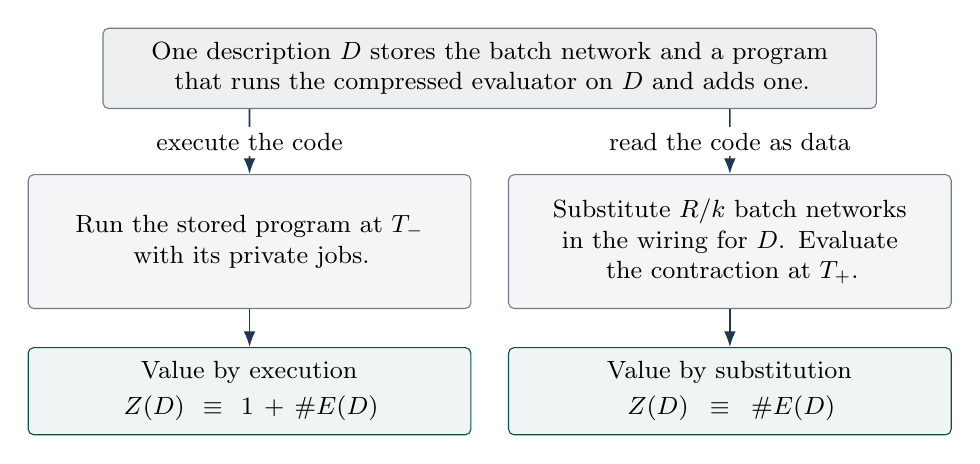
\begin{tikzpicture}[
  font=\small,
  box/.style={draw=ink!65,rounded corners=2pt,align=center,
              inner xsep=6pt,inner ysep=5pt},
  clockstage/.style={box,fill=ink!5,text width=5.2cm,minimum height=1.7cm},
  clockvalue/.style={box,fill=sea!7,draw=sea!70!black,text width=5.2cm},
  arrow/.style={-{Latex[length=2mm]},semithick,draw=ink}]
\node[box,fill=ink!8,text width=9.4cm] (description) at (0,0)
  {One description $D$ stores the batch network and a program\\
   that runs the compressed evaluator on $D$ and adds one.};
\node[clockstage] (run) at (-3.05,-2.2)
  {Run the stored program at $T_-$\\ with its private jobs.};
\node[clockstage] (wire) at (3.05,-2.2)
  {Substitute $R/k$ batch networks\\ in the wiring for $D$. Evaluate\\
   the contraction at $T_+$.};
\node[clockvalue] (runvalue) at (-3.05,-4.1)
  {Value by execution\\[2pt] $Z(D)\equiv 1+\#E(D)$};
\node[clockvalue] (wirevalue) at (3.05,-4.1)
  {Value by substitution\\[2pt] $Z(D)\equiv \#E(D)$};
\draw[arrow] ([xshift=-3.05cm]description.south) --
   node[midway,fill=white,inner sep=2pt]{execute the code} (run.north);
\draw[arrow] ([xshift=3.05cm]description.south) --
   node[midway,fill=white,inner sep=2pt]{read the code as data} (wire.north);
\draw[arrow] (run.south) -- (runvalue.north);
\draw[arrow] (wire.south) -- (wirevalue.north);
\end{tikzpicture}
\caption{Two evaluations of the same pinned contraction in
Theorem~\ref{thm:batches}. The evaluator $E$ on the right counts the
substituted network modulo $p$ for any public code in $D$. Compression
lets the program on the left run that count on its own stored
description and contribute one additional acceptance.}
\label{fig:clock}
\end{figure}


\section{Counting the coefficients of a formal circuit}\label{sec:parse}

A circuit that computes $P_n^*$ exactly supplies a coefficient for each
input to a signed processor. A border circuit supplies a point in the
closure of a family of coefficient vectors. To use such a point in the
clock argument, we first replace every processor entry by a polynomial
in a common set of scalar parameters $X$. Each path of the resulting
contraction contributes a monomial in $X$. Counting the paths that
contribute a given monomial will let us apply the compression of
Theorem~\ref{thm:gap}.

Assume for contradiction that $\bsz_F^{[n]}(P_n^*)\le m_0$, where
\[
 m_0=\lfloor 2^{n^\sigma}\rfloor,\qquad
 R=2^{\lceil n^\rho\rceil},\qquad M=m_0+n+w .
\]
Here $0<\sigma<\rho$ and $w$ is the word length from
Section~\ref{sec:gap}. Thus $M^C=o(R)$ for every fixed $C$.
The coefficient vector of $P_n^*$ is defined over the prime field.
The border hypothesis holds over its algebraic closure, since the
kernels of the circuit coefficient maps commute with field extension,
as in Section~\ref{sec:comparison}.

\subsection{One table for all circuits of a given size}
A coefficient query at $x\in\{0,1\}^n$ asks for the coefficient of
$\prod_i Z_{i,x_i}$. We parametrize the entire degree-$n$ output,
including the coefficients outside this set. The recursive form of the
parametrization will allow all $R$ processors to answer their queries
within the larger clock.

\begin{lemma}[Parse tables]\label{lem:parse-tables}
For every $n\ge1$ and $s\ge 1$ there is an integral polynomial map
$Y(X)$ from $h=(n+s)^{O(1)}$ scalar parameters to the full space of
degree-$n$ coefficients in $2n$ variables. In every field, the image
contains the degree-$n$ parts of all circuits of size at most $s$.
Each coordinate of $Y$ has degree at most $2n-1$ in $X$, and its
coefficient $\ell^1$-norm has logarithm $O(n\log(n+s+2))$ when nonzero.
\end{lemma}
\begin{proof}
Reserve $G=O(n+s)$ gate slots, including the used inputs and a
distinguished output. For each slot $g$ define $T_{g,1}$ to be a
linear combination of the $2n$ variables, with a separate parameter
for every coefficient. Recursively define
\[
 T_{g,d}=\sum_{e=1}^{d-1}\sum_{a,b=1}^{G}
     X_{g,d,e,a,b}\,T_{a,e}T_{b,d-e}\qquad (2\le d\le n).
\]
Take the coefficients of $T_{\mathrm{out},n}$ for the coordinates of
$Y$. The table has $O(nG+n^2G^3)$ parameters.

To encode a particular circuit, evaluate its degree-zero gate
components first. At each positive degree $d$, addition, subtraction
and multiplication by a degree-zero component give linear combinations
of earlier degree-$d$ components. Expand these linear dependencies in
topological order. At degree one the resulting expressions are linear
forms in the input variables. At degree $d\ge2$ they are linear
combinations of products of two positive-degree components with degrees
summing to $d$. Their coefficients give the required parameter values.

Expand the recursion before specializing any parameter. Each summand
corresponds to an ordered full binary tree with $n$ leaves. At each
internal node choose a split and two child slots. At each leaf choose
an input variable. A tree therefore contributes a product of $2n-1$
parameters. There are fewer than $4^n$ tree shapes, each with at most
$(n+s+2)^{O(n)}$ labelings. Collecting terms gives the asserted norm
bound, including multiplicities when two trees yield the same monomial.
\end{proof}

\subsection{Counting a coefficient of the contraction}
Fix the private machine of Theorem~\ref{thm:gap}(2) and the
$R$-processor wiring of Theorem~\ref{thm:gap}(1). The public description
$D$, including its code, uses at most $R/10$ active words. Set all
other description words to zero. Write $F_D(y)$ for the contraction
with these pins when each processor with input $x$ contributes the
coordinate $y_x$ indexed by $\prod_i Z_{i,x_i}$. In particular
$F_D(c)=Z(D)$, the genuine completed success count, for the full
coefficient vector $c$ of $P_n^*$.

At size $s=m_0$ the substituted contraction is
\[
 A_D(X)=F_D(Y(X)),\qquad \deg_X A_D\le L:=R(2n-1).
\]
Indeed, each assignment of the linked bits yields a product of $R$
coordinates of $Y$. All coefficients of $A_D$ are nonnegative integers.
Its value at the boundary will be recovered only after these terms
are summed.

\begin{lemma}[Coefficient counts]\label{lem:substitution}
Given $D$ and an exponent vector $\mu\in\mathbb Z_{\ge0}^{h}$ with
$|\mu|\le L$, a binary-guess program without private jobs at cap
$T_+$ has exactly $[X^\mu]A_D$ successful paths. The encoding of
$\mu$ uses $M^{O(1)}$ bits. The assertion holds for sufficiently small
$\rho$ with $0<\sigma<\rho$.
\end{lemma}

\begin{proof}
Generate the pins and wiring from $D$ and guess the linked bit
values. At each of the resulting $R$ inputs $x$, guess an ordered
tree from Lemma~\ref{lem:parse-tables}. Encode its $2n-1$ nodes in
preorder. Each record specifies a gate slot and degree. A leaf gives
its input variable, and an internal node gives its degree split and
ordered child slots. Check all ranges, the root slot and degree, and
require unused record fields to be zero.

A degree-$d$ node at position $u$ occupies $[u,u+2d-2]$ within
its block. For a split $d=e+(d-e)$ check the child records at
$u+1$ and $u+2e$. Their intervals partition the rest of the parent's
interval. Induction from the root therefore verifies every record
exactly once. Tally the leaf variables and require the monomial to be
$\prod_i Z_{i,x_i}$. Across all trees, tally the uses of every
parameter in a common random access array and require the totals
to equal $\mu$. A successful path specifies one wiring assignment and
one labeled ordered tree at each processor, exactly the multiplicity
with which that choice occurs in $[X^\mu]A_D$.

Each count, slot label or address fits in $O(w)$ bits. Initializing and
comparing the parameter totals costs $M^{O(1)}$, since the table has
$m_0^{O(1)}+n^{O(1)}$ parameters and $\log(L+1)=O(w)$. Generating the
wiring, checking the records and tallying the leaf variables takes
$O(Rn\operatorname{poly}(w))$ ticks. The exponent on $w$ is fixed, so
decreasing $\rho$ makes this term fit $T_+$, while $M^{O(1)}=o(R)$.
\end{proof}

Theorem~\ref{thm:gap}(2) now gives a smaller-clock simulation of each
coefficient count. Its compressor parameters have fixed values. The
parse-table parameters $X$ still have to account for a boundary point
$c$ of the image of $Y$, possibly with no assignment $X$ for which
$Y(X)=c$.

Sections~\ref{sec:descent} and~\ref{sec:cartier} recover this boundary
value through matrices over a prime field. One matrix $W_\mu$ will
represent each monomial $X^\mu$. The same nonzero vector $\Omega$ will
satisfy
\[
 \biggl(\sum_\mu ([X^\mu]A_D)\,W_\mu\biggr)\Omega=Z(D)\Omega
\]
for every description $D$. The computation can guess $\mu$ and count
one matrix entry using only polynomially many bits in $M$. In
Section~\ref{sec:border} it will supply one index as part of its own
description and guess the other. The vector $\Omega$ enters there
only through the displayed identity and the choice of one index at
which it is nonzero.

\section{A curve through the prescribed coefficients}\label{sec:descent}

An exact circuit gives a single choice of parse-table entries that realizes
all the coefficients of $P_n^*$. A border circuit gives a point in the
closure of the coefficient image. We realize that point as the value of the
whole table along one branch of an algebraic curve. At the chosen place,
the table entries may have poles, but every output coefficient is regular.
For example, the map $(x,y)\mapsto(x,xy)$ takes $(t,t^{-1})$ to
$(t,1)$. The value $(0,1)$ at $t=0$ has no finite preimage.
For the parse table, the processors in Section~\ref{sec:cartier} will
need equations for the curve and a short procedure for evaluating them.

Fix the compressor identities of Section~\ref{sec:compr} in the given
characteristic. Suppose that $\bsz_F^{[n]}(P_n^*)\le m_0$, with $m_0,M,R$
as in Section~\ref{sec:parse}. In this and the next two sections,
\emph{polynomial} means $M^{O(1)}$ and \emph{single exponential} means
$2^{M^{O(1)}}$. The exponents may depend on the fixed identities and are
uniform in $n$. Recall that $M^C=o(R)$ for every constant $C$.

Let $c=(c_\nu)_{|\nu|=n}$ be the integer coefficient vector of $P_n^*$
and write the table of Lemma~\ref{lem:parse-tables} at size $m_0$ as
\[
 T_X(Z)=\sum_{|\nu|=n}Y_\nu(X)Z^\nu,\qquad X=(X_1,\ldots,X_h).
\]
Here $Z$ lists all $2n$ paired input variables and $\nu$ ranges over
\emph{every} monomial of degree $n$. The closure of the coefficient
image contains $c$, interpreted over the algebraic closure of the prime
field as in Section~\ref{sec:parse}. The number $h\ge1$ is polynomial,
and each $Y_\nu$ has degree at most $d=2n-1$ and, when nonzero,
coefficient $\ell^1$-norm of polynomial bit length. The clock defining
$U_n^*$ gives the same bit bound for the entries of $c$.

\subsection{Specialization in characteristic zero}

To read a boundary value by residues we will work in positive
characteristic. In characteristic zero we can choose a prime separately
for each $n$. The prime must preserve the closure membership and have
bit length small enough for the processors.

\begin{lemma}\label{lem:descent-prime}
If $c\in\overline{Y(\mathbb A^h)}$ over $\overline{\mathbb Q}$, there is a
prime $p$ of polynomial bit length for which the same inclusion holds over
$\overline{\mathbb F}_p$. The fixed tensor identities can be specialized
at the same prime, with coefficients of bounded extension degree.
\end{lemma}

We use the following degree estimates over algebraically closed fields
(see \cite[Ch.~I, \S7]{Hartshorne} and
\cite[Lemma~2 and Proposition~3]{Heintz}).
For an affine variety we take the degree of its projective closure.
A linear image of an irreducible variety has closure of degree at most
the degree of the variety. For a rational map on an open subset of
$\mathbb A^h$ whose numerators and common denominator have degree at most
$e\ge1$, the degree of the image closure is at most $e^h$. Indeed, a
general linear section of complementary dimension meets the image closure
in $D'$ distinct points of the image, where $D'$ is the degree of the
closure. In the domain its pullback has at least one component over
each point. B\'ezout bounds the number
of components by $e^h$, even in mixed dimensions. At each cut of degree
at most $e$, the sum of $(\deg V)e^{\dim V}$ over the components $V$
cannot increase. In particular, linear sections never increase the sum
of component degrees.

We will also use that a closed irreducible set of degree $D$ can be
separated from any point outside it by an equation of degree at most $D$.
For a set of dimension $b$ and codimension at least two, project its
projective closure to $\mathbb P^{b+1}$ from a linear center disjoint from
its join with the point. The image misses the projected point and has
dimension $b$, since a positive-dimensional projective fiber would meet the
center. Its hypersurface equation pulls back to the required separator.
In codimension one the defining equation suffices. For a reducible set,
multiply the separators for its components.

\begin{proof}[Proof of Lemma~\ref{lem:descent-prime}]
The image closure has degree at most $D=d^h$ in every characteristic.
It therefore suffices to preserve the vanishing at $c$ of all relations
of degree at most $D$. Record substitution $y\mapsto Y(X)$ on these
polynomials by an integer matrix $A$. Its column for $y^\eta$ is the
coefficient vector of $Y(X)^\eta$ in $X$-monomials of degree at most
$dD$. The row $u=(c^\eta)_{|\eta|\le D}$ records evaluation at $c$.
The rational kernel of $A$ consists of the relations, so the closure
hypothesis puts $u$ in the rational row span.

There are only $\binom{h+dD}{h}$ rows, a single exponential, regardless
of the number of columns. Submultiplicativity of the coefficient norm
bounds the bit length of each matrix entry by a single exponential.
Choose a row basis and a square minor on those rows with nonzero
determinant $\Delta$. Cramer's rule expresses $u$ in the basis with
denominators dividing $\Delta$. The expression obtained on the minor's
columns holds on all columns because $u$ is in the row span. Hadamard's
inequality gives a singly exponential bound on the bit length of $\Delta$.

The constants of the fixed identities lie in a fixed number field and
are integral after inverting a fixed integer. Outside a finite list of
primes we may reduce at any prime ideal over $p$, preserving both the
identities and any required nonvanishings. The residue degree is at most
the number-field degree. Some prime $p$ of polynomial bit length lies
outside this list and does not divide $\Delta$, since the logarithm of
the product of all primes up to $x$ is asymptotic to $x$. Reducing the row
expression now puts $u\bmod p$ in the row span of $A\bmod p$. It therefore
annihilates every relation of degree at most $D$ even over
$\overline{\mathbb F}_p$. The separator bound proves the inclusion.
\end{proof}

In the diagonal argument the compressor identities were chosen over the
prime field in Section~\ref{sec:compr}. Their characteristic-zero
constants are rational, so the specialization above places them in
$\mathbb F_p$. The original layouts therefore give the same contraction
identities over $\mathbb F_p$, whether or not this new characteristic
admits ports. In fixed positive characteristic we keep the original
prime and constants. In both cases write $\mathcal K=\overline{\mathbb F}_p$
and let $E_0$ be a finite field containing the constants, of degree over
$\mathbb F_p$ bounded independently of $n$. For the prime-field choices
we can take $E_0=\mathbb F_p$.

\subsection{Equations for the branch}

Lehmkuhl and Lickteig for tensors, and B\"urgisser for circuits, used
the degree of the graph of a parameter map to bound the order of
approximation \cite{LehmkuhlLickteig,BurgisserCorrection}. Guo, Saxena and
Sinhababu give the corresponding classical bounded-degree approximation
for approximate polynomial satisfiability over arbitrary fields
\cite[Theorem~4.2]{GSS}. Here we need a separable curve parameter $t$
and equations that the processors can evaluate in polynomial time.

\begin{proposition}\label{prop:descent-curve}
There are a finite extension $E$ of $E_0$, with $\log_2|E|$ polynomial, and
$h$ polynomials $g_i(X,t)\in E[X,t]$ of polynomial degree with the following
properties. Their common zero set over $\mathcal K$ has an irreducible curve
component of singly exponential degree, dominant over the $t$-line, on which
$J=\det(\partial g_i/\partial X_j)$ is generically nonzero. The function
field of this curve has a place above $t=0$ at which all $Y_\nu$ are regular
with residue $c_\nu$. With polynomial advice, each $g_i$ can be evaluated
in polynomial bit time over $E$ or a specified extension of polynomial bit
length, given its field representation and the embedding of $E$.
\end{proposition}

\begin{proof}
Close the graph of $Y$ in $\mathbb P^h\times\mathbb A^{\{\nu:|\nu|=n\}}$
using homogeneous parameter coordinates $(1:X)$. The projection to output
space is closed, so the fiber above $c$ is a nonempty projective set,
possibly entirely at parameter infinity. On each standard parameter
chart the graph closure has degree at most $(d+1)^h$. Indeed, its dense
finite-parameter part is parametrized by $X$ with chart coordinates
given by ratios of affine linear forms and output coordinates $Y(X)$.
With the chart denominator common to all coordinates, the numerators
have degree at most $d+1$. The fiber above $c$ is a linear section on
each chart. Counting each projective component in a chart meeting it
bounds the sum of the fiber component degrees by $(h+1)(d+1)^h$.

Cut the projective fiber by parameter hyperplanes until it is finite.
At each cut avoid the hyperplanes containing a positive-dimensional
component. Every such component meets the chosen hyperplane by
projectivity, so the last intersection is still nonempty. Each component
excludes at most a proper linear subspace of coefficients, and the
number of exclusions at a cut is bounded by the degree sum above.
Fix a point $P$ of the finite intersection and a standard chart containing
it. Denote the graph closure in this chart by $G$, write $(z,y)$ for the
chart and output coordinates, and let $\ell_1(z),\ldots,\ell_b(z)$ be
the hyperplanes used in the cuts. On $G$, the common zeros of the forms
$y_\nu-c_\nu$ and $\ell_j$ now make up a finite set containing $P$.

We need $h$ equations for a finite intersection, with short descriptions
even when the table has many output coordinates. Encode each $\nu$ by
its base-$(n+1)$ digits. With $B=(n+1)^{2n}$, put
\[
 e(\nu)=\sum_{j=1}^{2n}\nu_j(n+1)^{j-1},\qquad
 D_a(z,y)=\sum_\nu a^{e(\nu)}(y_\nu-c_\nu)
             +\sum_{j=1}^b a^{B+j}\ell_j(z).
\]
On any surviving positive-dimensional component, at least one original
form is nonzero at some point. At that point $D_a$ is a nonzero
polynomial in $a$ of degree at most $B+b$, because all the exponents
are distinct. Avoiding its roots for each such component cuts every
positive dimension by one. These are linear cuts on $G$, so at each
step there are at most $\deg G$ components. After $h$ choices
$a_1,\ldots,a_h$, the common zeros of $D_i=D_{a_i}$ form a finite
set containing $P$.

We now deform this intersection. For a vector $v$ to be chosen, impose
\begin{equation}\label{eq:descent-deform}
                    D_i(z,y)+t(z_i-v_i)=0\qquad(1\le i\le h).
\end{equation}
At $t=0$ these equations retain $P$. Over $\overline{\mathcal K(t)}$,
they cut out the fiber over $v$ of the affine linear map
$\psi_t(z,y)=z+t^{-1}D(z,y)$, where $D=(D_1,\ldots,D_h)$.
Let $U\subset G$ be the finite-parameter part of this chart. It is an
open subset of $z$-space, with $y=Y(X(z))$. Write
$\widetilde D(z)=D(z,Y(X(z)))$. The determinant
$\det(tI+\partial\widetilde D/\partial z)$ is monic in $t$ over
$\mathcal K(G)$. Thus its vanishing on $U$ cuts out a set of dimension
less than $h$ over the generic $t$, even if the derivatives of all
outputs vanish in characteristic $p$.

Choose $v$ outside the closures of the images under $\psi_t$ of this
critical locus and of $G\setminus U$. They lie in a hypersurface of
singly exponential degree. Indeed, $G\setminus U$ is empty or cut out
by one chart coordinate. Each $\widetilde D_i$ has numerator of degree
at most $d+1$ and denominator a common linear form to power $d$.
Clearing the denominators in the determinant gives a polynomial of
degree $O(h(d+1))$ in $z$. By B\'ezout the sum of the degrees of the
two exceptional loci, after closure, is $O(h(d+1))\deg G$. Taking
linear images and multiplying their component separators gives a
hypersurface of at most this degree. Consequently every point
of the generic fiber has finite parameters and invertible $z$-Jacobian.

All hyperplane coefficients, the $a_i$ and $v$ can be chosen in one
extension $E$ of $E_0$ whose elements have polynomial bit length.
At every stage the product of the equations to be avoided has singly
exponential degree, uniformly in the earlier choices. A grid in a field
of size larger than that degree contains a point where the product is
nonzero, including for the exceptional hypersurface over
$\overline{\mathcal K(t)}$. Since $\log_2|E_0|$ is polynomial, we
can take a finite extension of this size with $\log_2|E|$ polynomial.

In $G\times\mathbb A^1$ the $h$ equations in
\eqref{eq:descent-deform} have local dimension at least one at $(P,0)$
by Krull's dimension theorem. Every component through that point of positive
dimension dominates the $t$-line, since the special fiber is finite.
The generic fiber has dimension at most zero by the invertible Jacobian,
so each such component is a curve. Choose one and take a point above
$(P,0)$ on its normalization. The functions $y_\nu$ are regular at
this place, with values $c_\nu$. On the dense finite-parameter part
they equal $Y_\nu(X)$, which therefore have the same values even if
some $X_j$ have poles.

It remains to give the equations in the original table entries $X$.
Write the chart coordinates as $z_i=u_i(X)/\delta(X)$ with $u_i$ and
$\delta$ affine linear. Clearing the denominator gives
\[
 g_i(X,t)=\delta(X) D_i\bigl(z,Y(X)\bigr)
                  +t\bigl(u_i(X)-v_i\delta(X)\bigr).
\]
This is polynomial because $D_i$ is affine linear in $z,y$. On the
finite-parameter chart the change of coordinates from $z$ to $X$ has
invertible Jacobian. At a common zero multiplying the equations by
$\delta$ scales each Jacobian row by a unit. Hence the affine closure
of the chosen curve in $X,t$ is a component with $J\ne0$ generically.
Its degree is at most $(d+2)^h$ by B\'ezout, since the equations have
degree at most $d+2$. The relations $dg_i=0$ express every $dX_j$ as
a multiple of $dt$. The curve has one-dimensional function-field
differentials over the perfect field $\mathcal K$, so $dt$ spans them.

For the evaluator, the large sum of output coordinates in each $D_i$
is just one table evaluation. For $a=a_i$,
\[
 \sum_\nu a^{e(\nu)}Y_\nu(X)
     =T_X\bigl(a^{(n+1)^0},\ldots,a^{(n+1)^{2n-1}}\bigr).
\]
Store the corresponding offset $\sum_\nu a^{e(\nu)}c_\nu$ as one
element of $E$. The $a_i$, hyperplane coefficients, $v$, offsets and
field arithmetic data take polynomially many advice bits. The exponents
have polynomial bit length, and Lemma~\ref{lem:parse-tables} supplies
the polynomial-size table recursion with weights $X$. Binary powering,
that recursion and the affine forms $u_i,\delta$ thus evaluate $g_i$
in polynomial bit time, using the cleared expression even at
$\delta(X)=0$. This evaluator uses only field data for the equations.
The geometric point $P$ and its branch may be defined over larger fields.
\end{proof}

\section{Reading a boundary value with residues}\label{sec:cartier}

Proposition~\ref{prop:descent-curve} gives a curve on which the output
coefficients $Y(X)$ have the required value $c$ at a place above $t=0$.
Individual parameter monomials can have poles there. For instance,
if $u=t^{-1}$ and $v=t^{-1}-t$, then $u^2$ and $uv$ both have poles
at $t=0$, yet $u^2-uv=1$. A counting path in
Lemma~\ref{lem:substitution} produces one monomial at a time. We need
a rule for combining its contributions that respects cancellation at
the chosen place.

We assign each weighted monomial $aX^\mu$ a matrix. For every regular
sum with a value in the prime field, the sum of its matrices acts by
that value on a single nonzero vector. In the example, the difference
of the two matrices acts as the identity on the vector. We use the size
parameter $M$ of Section~\ref{sec:descent} throughout.

\begin{lemma}[Matrices for the boundary value]\label{lem:pins}
Fix a singly exponential degree bound $L$. There are a nonzero vector
$\Omega\in\mathbb F_p^d$ and matrices $W_{a,\mu}\in\mathbb F_p^{d\times d}$
for $a\in E$ and $\mu\in\mathbb Z_{\ge0}^{h}$ with $|\mu|\le L$.
If $A=\sum_\mu a_\mu X^\mu\in E[X]$ has degree at most $L$, is
regular at the chosen place and has value $z\in\mathbb F_p$ there, then
\begin{equation}\label{eq:cartier-pin}
                 \biggl(\sum_\mu W_{a_\mu,\mu}\biggr)\Omega=z\Omega .
\end{equation}
In particular, this holds for $A=F(Y(X))$ of degree at most $L$,
with $F$ over $\mathbb F_p$ and $z=F(c)$. For fixed $\mu$ the matrix
is $\mathbb F_p$-linear in $a$, and $d$ is singly exponential. With
one polynomial-length advice string for all $a,\mu$ and all pairs of
indices, any specified entry is the number modulo $p$ of accepting
paths of a polynomial-time binary-guess computation.
\end{lemma}

The entries of $\Omega$ will be residues of test differentials on
the curve, followed by a field trace. If $A$ has boundary value
$z\in\mathbb F_p$, then $A^q-z=(A-z)^q$ vanishes to order at least
$q$ for every $p$-power $q$. For a test differential $\eta$ with pole
order less than $q$, it follows that $A^q\eta$ and $z\eta$ have the same
residue. The Cartier operator converts this observation into a rule
linear in $A$, through the identity $C_q(A^q\eta)=A C_q(\eta)$.
Speyer represented transitions of finite automata by related operators
on curve differentials. Bridy used this interpretation to bound the
number of states~\cite[Proposition~3.8 and Theorem~1.2]{Bridy}.
Here the tests must admit matrix entries that a counting path can
evaluate in the coordinates of the given curve equations.

\subsection{From the local coordinate to the curve equations}

Write $x=(x_1,\ldots,x_h)$ for the coordinate functions on the
geometric curve and $K=E(t,x)$ for the field they generate over $E$.
It is finite over $E(t)$. Indeed, each $x_i$ is algebraic over
$\overline{\mathbb F}_p(t)$, and only finitely many algebraic constants
occur in a defining equation for it. Restrict the chosen valuation to
$K$ and normalize its value group to $\mathbb Z$. Its residue field
$\kappa$ is finite, since the place lies over $t=0$ in a finite
function field extension. The residues of $Y(x)$ are still $c$.

Choose a uniformizer $s\in K$ at this place. The completion is
$\kappa((s))$, with the coefficient field obtained by lifting the
roots of $T^{|\kappa|}-T$. Put
\[
   J=\det\left(\frac{\partial g_i}{\partial X_j}\right),\qquad
   \eta_0=\frac{dt}{J(x,t)} .
\]
The Jacobian is nonzero at the generic point by
Proposition~\ref{prop:descent-curve}. Differentiating $g_i(x,t)=0$
expresses every $dx_j$ as a multiple of $dt$. In particular, $ds$
is a multiple of $dt$ because $s\in E(t,x)$. As $ds\ne0$ in
$\kappa((s))$, the differential $\eta_0$ is nonzero even when
$t$ is ramified at the branch.

Write $\operatorname{Res}\eta$ for the coefficient of $s^{-1}ds$ in
$\eta$. For $q=p^u$, $u\ge1$, Cartier acts in the local coordinate by
\[
 C_q\!\left(\sum_j v_j s^j\,ds\right)
       =\sum_i v_{q i+q-1}^{1/q}s^i\,ds .
\]
Grouping exponents modulo $q$ gives $C_q(D^q\eta)=D C_q(\eta)$,
and the coefficient at $i=-1$ gives
$\operatorname{Res}(C_q\eta)=(\operatorname{Res}\eta)^{1/q}$.
In the ambient coordinates $Z=(X_1,\ldots,X_h,t)$ put
\[
   \Lambda_q\!\left(\sum_j v_j Z^j\right)
        =\sum_i v_{q i+(q-1)\mathbf1}^{1/q} Z^i .
\]
This operator retains exponents congruent to $q-1$ in every
coordinate. The next formula computes the local action using only
this coefficient extraction and the defining equations of the curve.

\begin{lemma}\label{lem:cartier-formula}
For $f\in E[X_1,\ldots,X_h,t,t^{-1}]$ one has
\begin{equation}\label{eq:cartier-adjunction}
 C_q\bigl(f(x,t)\eta_0\bigr)
       =\Lambda_q\!\left(f\prod_{i=1}^h g_i^{q-1}\right)(x,t)\,\eta_0 .
\end{equation}
\end{lemma}

\begin{proof}
For a plane curve this is the formula of St\"ohr and
Voloch~\cite[Theorem~1.1]{StoehrVoloch}. The coordinate change in
higher codimension uses the naturality of Cartier on top
differentials~\cite{Cartier,Katz}. Recall its coefficient description.
In coordinates $z_1,\ldots,z_b$ forming a $p$-basis, each element
has a unique expansion in $z^j$, $0\le j_i<p$, over the subfield
of $p$-th powers. In a top form all terms with some $j_i<p-1$ have
an antiderivative in that coordinate. An exact form has zero
coefficient at $j=(p-1)\mathbf1$. Thus precisely this coefficient
survives modulo exact top forms. The intrinsic inverse Cartier map
from top forms to this quotient sends
\[
 a\,dv_1\wedge\cdots\wedge dv_b\longmapsto
 \left[a^p\bigwedge_{i=1}^b v_i^{p-1}dv_i\right].
\]
Indeed, $v^{p-1}dv$ is closed, obeys the product rule with scalars
raised to the $p$-th power, and is additive modulo exact forms.
The correction for additivity is the differential of the reduction
of the integral polynomial $((U+V)^p-U^p-V^p)/p$. This construction
commutes with the field embedding below, and inversion gives the
coefficient rule for Cartier. Iteration gives the rule for $q$.
In an iterated Laurent series field over a perfect field, grouping
exponents modulo $p$ shows that the series variables form a $p$-basis.

Introduce independent variables $y_1,\ldots,y_h$ over $\kappa((s))$.
Since $J(x,t)$ is invertible there, the formal implicit function
theorem gives $\widetilde x\in\kappa((s))[[y_1,\ldots,y_h]]^h$
with $\widetilde x(0)=x$ and $g_i(\widetilde x,t)=y_i$.
Hence $X\mapsto\widetilde x$, $t\mapsto t(s)$ embeds the ambient
rational function field in the iterated Laurent series field. Indeed,
the image contains the algebraically independent elements
$t(s),y_1,\ldots,y_h$. In the new variables the volume form is
\[
 dX_1\wedge\cdots\wedge dX_h\wedge dt
    = J(\widetilde x,t)^{-1}dy_1\wedge\cdots\wedge dy_h\wedge dt .
\]
Multiply by $f\prod_i g_i^{q-1}$ and apply Cartier. In the ambient
coordinates its coefficient becomes $\Lambda_q(f\prod_i g_i^{q-1})$.
In the series coordinates the factor $\prod_i y_i^{q-1}$ shifts
the constant term of $f(\widetilde x,t)/J(\widetilde x,t)$ to
$y^{(q-1)\mathbf1}$. This term alone contributes to the constant
$y$-coefficient after Cartier. Since $dt=t'(s)ds$, that coefficient
times $ds$ is $C_q(f(x,t)\eta_0)$. In the ambient calculation it is
$\Lambda_q(f\prod_i g_i^{q-1})(x,t)\eta_0$. This yields
\eqref{eq:cartier-adjunction}.
\end{proof}

\subsection{A finite family of test differentials}

We need a family large enough to detect a nonzero residue, whose span
is stable under each combined operation $\eta\mapsto a x^\mu C_q(\eta)$
with $|\mu|\le L$. Set $S=\sum_i\deg g_i$, $H=4(L+S+2)$, and take
the box of monomials
\[
  \mathcal B=\{X^\alpha t^j\mid 0\le\alpha_i\le H,\ -H\le j\le H\}.
\]
For $f\in\mathcal B$, $a,b\in E$ and $|\mu|\le L$, the Laurent polynomial
\begin{equation}\label{eq:cartier-row}
       aX^\mu\Lambda_q\!\left(bf\prod_i g_i^{q-1}\right)
\end{equation}
is supported in $\mathcal B$. In fact, the product with
$\prod_i g_i^{q-1}$ increases each upper exponent by at most
$(q-1)S$. After extraction and multiplication by $X^\mu$, the upper
bound in each coordinate is at most $H/q+S+L\le H$. The extracted
$X$ exponents are nonnegative, and the lower $t$ exponent is at least
$-H/q-1\ge-H$.

To bound pole orders of the tests, let $D$ be the degree of the
geometric curve. B\'ezout gives $D\le\prod_i\deg g_i$, which is
singly exponential by Proposition~\ref{prop:descent-curve}. On the
normalized projective model, a quotient of polynomials of degrees at
most $e$ has poles of order at most $eD$, provided its denominator
does not vanish identically on the curve. Homogenizing to a common
degree bounds the pole divisor by the intersection with the
denominator hypersurface. For $f/J$ one can take $e=(h+2)H+S$
after clearing negative powers of $t$. Restricting the valuation
to $K$ and normalizing only decreases this bound on pole orders.
Also $dt$ is regular since $t$ has positive valuation. Take $q$
to be the first positive power of $|E|$ exceeding $e\prod_i\deg g_i$.
This singly exponential $q$ works simultaneously for all the differentials
$f(x,t)\eta_0$ and fixes the scalars in $E$ under $q$-th powering.

Fix an $\mathbb F_p$-basis of $E$. Use pairs $(b,f)$ of a basis
element and a box monomial as our indices, and put
\[
 \ell(\eta)=\operatorname{Tr}_{\kappa/\mathbb F_p}(\operatorname{Res}\eta),
 \qquad \Omega(b,f)=\ell\bigl(bf(x,t)\eta_0\bigr).
\]
These entries are in $\mathbb F_p$, and $\ell(C_q\eta)=\ell(\eta)$
because the absolute trace is invariant under inverse Frobenius.

We show that the box contains a test with nonzero traced residue.
Choose a trace-one element of the finite separable extension
$\kappa/\mathbb F_p$ and lift it to an element $w$ of the valuation
ring of $K$. Then $\ell(w\,ds/s)=1$. The quotient
$(w\,ds/s)/\eta_0$ is in $K$. Express it as a finite linear combination
of monomials in $x$ with coefficients in $E(t)$, using the finiteness
of $E(t,x)/E(t)$. Approximate each rational coefficient by a Laurent
polynomial in $t$ over $E$. Since $t$ has positive valuation, sufficiently
long approximations preserve the residue after multiplication by the
finitely many test factors $x^\alpha\eta_0$. This gives a Laurent
polynomial $f_0\in E[X,t,t^{-1}]$ with $\ell(f_0(x,t)\eta_0)=1$.

The exponents of $f_0$ need not yet lie in $\mathcal B$. Apply
Lemma~\ref{lem:cartier-formula} with a $p$-power $Q$ larger than
the absolute values of all these exponents. The polynomial
$\Lambda_Q(f_0\prod_i g_i^{Q-1})$ is supported in $\mathcal B$ by the
same exponent bound, and its traced residue against $\eta_0$ is still
one. Expand its coefficients in the chosen basis of $E$. At least
one of the resulting entries $\Omega(b,f)$ is nonzero. The power $Q$
and the local functions $w,s$ serve only to prove this existence.
The matrix entries below use the uniform power $q$ and the curve equations.

\subsection{The matrix action and its entry counts}

\begin{proof}[Proof of Lemma~\ref{lem:pins}]
In row $(b,f)$ of $W_{a,\mu}$, enter the coefficients of
\eqref{eq:cartier-row} in the basis $b'f'$, with columns indexed
by $(b',f')$. The support bound makes this a square matrix over
$\mathbb F_p$. Multiplication by $a$ after extraction makes the
row $\mathbb F_p$-linear in $a$. By
Lemma~\ref{lem:cartier-formula}, the $(b,f)$ entry on the left of
\eqref{eq:cartier-pin}, with evaluations on the curve understood, is
\[
   \ell\!\left(A\,C_q(bf\eta_0)\right)
    =\ell\!\left(C_q(A^q bf\eta_0)\right)
    =\ell(A^q bf\eta_0)=z\,\ell(bf\eta_0).
\]
The last equality uses regularity of the whole sum $A$. The zero
of $A^q-z$ has order at least $q$, so $(A^q-z)bf\eta_0$ has zero
residue. This proves \eqref{eq:cartier-pin}. More generally, if
the boundary value is $z\in E$, then $z^q=z$ and the right side
becomes $R_z\Omega$, where row $(b,f)$ of $R_z$ expands $zb$ in
the fixed basis while keeping $f$ fixed.

There are $d=[E:\mathbb F_p](H+1)^h(2H+1)$ indices, each of
polynomial bit length. To compute an entry in row $(b,f)$ and
column $(b',f')$, subtract $(\mu,0)$ from the exponent vector of
$f'$ and call the difference $i$. With
\[
       j=qi+(q-1)\mathbf1,\qquad V=bf\prod_i g_i^{q-1},
\]
the requested entry is the $b'$-coordinate of $a[Z^j]V$. The
inverse Frobenius in $\Lambda_q$ fixes $E$ since $q$ is a power
of $|E|$. If $j$ lies outside the exponent vector of $f$ plus
the box $[0,(q-1)S]^{h+1}$, the entry is zero.

Otherwise take the finite extension $E'/E$ of least positive degree
such that $N=|E'|-1>(q-1)S$. Its elements have polynomial bit length,
since $|E'|\le |E|((q-1)S+2)$. Orthogonality in $(E')^\times$
gives
\[
       [Z^j]V=N^{-(h+1)}
           \sum_{z\in((E')^\times)^{h+1}} V(z)z^{-j}.
\]
Every coordinate interval of the support has width less than $N$.
Thus the only exponent of the support that can be congruent to $j$
modulo $N$ in all coordinates is $j$ itself. The argument applies
also to the negative powers of $t$.

Give the counting procedure the curve evaluators from
Proposition~\ref{prop:descent-curve}, the exponent defining $q$, field
presentations, embeddings, and basis data as polynomial-length advice. A path guesses one tuple
of nonzero elements of $E'$ in canonical encodings, rejecting invalid
guesses. It evaluates $V(z)z^{-j}$ and the normalization factor by
the curve evaluators and binary powering. Multiply by $a$ and apply
the coordinate projection for $b'$, extended $\mathbb F_p$-linearly
from $E$ to $E'$. Both operations take polynomial time and commute
with the sum over tuples. If the resulting prime-field element has
integer representative $v\in[0,p-1]$, a final guess of
$\lceil\log_2 p\rceil$ bits accepts exactly when its value is less
than $v$. Each summand therefore contributes the required number
of accepting paths modulo $p$.

We may pad $d$ to the next power of two by adding zero rows and
columns to the matrices and zero coordinates to $\Omega$. The
entry procedure then takes binary indices of one fixed length.
Section~\ref{sec:border} uses one such index at which $\Omega$ is
nonzero and the entry procedure common to all the monomials.
\end{proof}

\section{From the boundary value to the circuit lower bound}\label{sec:border}

\begin{proof}[Proof of Theorem~\ref{thm:stretch}]
Fix a characteristic admitting ports and the corresponding compressor
identities and clocks. Suppose that at a sufficiently large $n$ the
coefficient vector of $P_n^*$ lies in the degree-component border of
circuits of size $m_0=\lfloor 2^{n^\sigma}\rfloor$. In positive
characteristic use the given prime $p$. In characteristic zero apply
Lemma~\ref{lem:descent-prime} to the parse table. It preserves the
image-closure inclusion and the fixed rational compressor identities
at a prime $p$ of polynomial bit length in $M$. This prime may
depend on $n$. In both cases we evaluate compressor constants in
$\mathbb F_p$.

Apply Lemma~\ref{lem:pins} on the curve of
Proposition~\ref{prop:descent-curve} with $L=R(2n-1)$. Write
$W_\mu=W_{1,\mu}$, use the padded binary indexing, and choose an
index $H_*$ at which $\Omega(H_*)\ne0$. All matrices, their entry
procedure and its advice are now fixed. Include $H_*$, the advice,
the size parameters and the public program in a description $D(H)$,
reserving one field for a variable index $H$. Define
\[
 \begin{aligned}
 Z(H)&=Z(D(H))\bmod p, & A_H&=A_{D(H)},\\
 W(H)&=\sum_{|\mu|\le L}([X^\mu]A_H)\,W_\mu .
 \end{aligned}
\]
For any choice of public program, $A_H=F_{D(H)}(Y(X))$ is regular on the
chosen branch and has value $F_{D(H)}(c)=Z(H)$. By linearity in the
coefficient in Lemma~\ref{lem:pins},
\begin{equation}\label{eq:border-row}
                   W(H)\Omega=Z(H)\Omega\qquad\text{for every }H .
\end{equation}
In particular, row $H$ of this identity computes $Z(H)\Omega(H)$.

Choose the public program on input $D(H)$ to count, modulo $p$,
\begin{equation}\label{eq:border-column}
  \mathbf 1_{\{H=H_*\}}+\sum_I W(I)_{I,H}
  =\mathbf 1_{\{H=H_*\}}+
       \sum_{I,\mu}([X^\mu]A_I)(W_\mu)_{I,H}.
\end{equation}
One branch accepts precisely when $H=H_*$. The other guesses $I$ and
a valid exponent vector $\mu$ in their canonical binary encodings and
replaces $H$ by $I$ in a copy of the description. Supply the active
words of $D(I)$ and the exponent vector $\mu$ as one input of at most
$R$ words, with the unused words of $D(I)$ understood as zero.
Lemma~\ref{lem:substitution} counts $[X^\mu]A_I$ from this input at
the larger clock. Simulate it
at the smaller clock with private jobs by Theorem~\ref{thm:gap}(2).
On each completed path, evaluate its tallied compressor monomial in
$\mathbb F_p$. A further binary guess smaller than its representative
in $[0,p-1]$ gives exactly that many successes. Independently, run the
entry procedure from Lemma~\ref{lem:pins} for $(W_\mu)_{I,H}$, requiring
both procedures to accept. This multiplies their counts. Summing over
the guesses gives \eqref{eq:border-column}.

The fixed private machine determines the wiring generator before we
choose the public program. The larger-clock procedure uses $D(I)$ as
data for the pins and links of that wiring. The smaller-clock program
constructs this input by copying its stored instructions and advice,
changing only the field for the index. Thus the same code works at
every $H$. The fixed code and the $M^{O(1)}$ bits of data fit within
the reserved $R/10$ active words for large $n$. Apart from the
$o(T_-)$ simulation and the $O(R)$ cost of copying the description,
the prime-field computations and the entry path cost $M^{O(1)}=o(R)$
ticks. The entire program therefore fits $T_-$.

By Theorem~\ref{thm:gap}(1), the success count of this program equals
$Z(H)$ in $\mathbb F_p$. Multiply \eqref{eq:border-column} by
$\Omega(H)$ and sum over $H$. Interchanging the finite sums groups
row $I$ with $\Omega$ in \eqref{eq:border-row}, giving
\[
 \sum_H Z(H)\Omega(H)
 =\Omega(H_*)+\sum_I\bigl(W(I)\Omega\bigr)_I
 =\Omega(H_*)+\sum_I Z(I)\Omega(I).
\]
Cancellation contradicts the choice of $H_*$. Hence
$\bsz_F^{[n]}(P_n^*)>2^{n^\sigma}$ for all sufficiently large $n$
in the chosen characteristic.

To transfer the bound, use the signed verifier of
Section~\ref{sec:model}. It accepts the paths with output $+1$ or
$-1$, gives the negative-output bit weight $-1$, and attaches the
selected variables $Z_{i,x_i}$ to its output bits. Its length is
polynomial in $n$. Lemma~\ref{gadget:verifier} projects $\HC$ of order
at most $A n^B$ to $P_n^*$, and supplies the same projection for
$\Per$ outside characteristic two, for fixed $A,B>0$. At order $N$,
take $n=\lfloor(N/A)^{1/B}\rfloor$ and pad the graph by a forced path
or an identity block, respectively. As in Section~\ref{sec:comparison},
extracting the degree-$N$ component of a size-$s$ approximant before
projection costs $O((N+1)^2(s+1))$. The projection and the final
degree-$n$ extraction preserve the closure. Consequently this polynomial
overhead times $s+1$ must exceed $2^{n^\sigma}$. Taking any fixed
$0<\varepsilon<\sigma/B$ gives the asserted $2^{N^\varepsilon}$
lower bound for all sufficiently large $N$.

Keeping a distinct variable on each edge of the verifier graph gives
the port case of Corollary~\ref{cor:sparse-support}. Specializing those
variables to the verifier weights gives precisely the projection above,
and the padding preserves the degree bounds on the support.
\end{proof}

\begin{proof}[Completion of the proof of Theorem~\ref{thm:main}]
In each characteristic without ports, the comparison in
Section~\ref{sec:comparison} gives the lower bound
$\exp\bigl(c(\log N)^2/(\log\log N)^2\bigr)$ with an absolute $c>0$.
In each characteristic admitting ports, Theorem~\ref{thm:stretch}
gives $2^{N^\varepsilon}$ for some $\varepsilon>0$ depending on that
characteristic. This exceeds the first bound with the same absolute
$c$ once $N$ is sufficiently large in the given characteristic.
The two cases exhaust all characteristics, including zero. They give
the stated bound for $\HC_N$ over every field and for $\Per_N$ over
every field of characteristic different from two.
\end{proof}


\bibliographystyle{plainnat}
\bookmarksetup{startatroot}
\bibliography{references}
\end{document}
